\chapter{Resultados}

\section{Levantamiento de información}
Por medio del levantamiento de información es posible hacer un pequeño análisis del estado actual y los datos obtenidos. Por un lado, la estructura actual responde a la necesidad de colocar la máquina en una ubicación transitoria, debido a los trabajos realizados en el piso del laboratorio durante el año 2012. Por lo mismo, no está diseñada para la operación de la máquina bajo ningún contexto por los peligros que conlleva. Aún cuando esta podría ser modificada, se desconocen las características y propiedades de la especie maderera con la que fue fabricada, lo que obliga a diseñar y construir un nuevo soporte para la máquina. 

Por otra parte, la información obtenida de la máquina de fatiga da cuenta de tres puntos importantes. La antigüedad de sus componentes y la tecnología utilizada afecta directamente en su mantenimiento ante la dificultad de encontrar piezas de repuesto, debido a que las dimensiones de sus componentes, como la polea y la correa, se encuentran fuera de catálogo o de las dimensiones de fabricación de los proveedores. También la obsolescencia de la tecnología tienen incidencia, siendo difícil poder encontrar no sólo las piezas de repuesto, sino que también personas que estén técnicamente calificadas. En segundo lugar, la máquina fue fabricada con estándares o líneas de desarrollo propias de la época, como sería esperable, las cuales no evolucionaron en la misma dirección que los estándares actuales de ensayo a fatiga, dificultando la comparación de los resultados obtenidos. Finalmente, la robustez del diseño, la cual se puede apreciar fácilmente en la dimensiones de la estructura exterior de la máquina, tiene la dualidad de proveer un armazón macizo y duradero sobre el cual trabajar, por el contrario, resulta ser una estructura difícil de modificar por esta misma razón.

En lo relativo a la exactitud de los datos obtenidos, la imposibilidad de desarmar gran parte de la máquina afectaron la precisión de las mediciones realizadas, sobre todo en partes específicas. Así, las dimensiones y la geometría de las vigas en voladizo tuvieron que ser simplificadas ante la imposibilidad de tomar medidas en la unión barra-disco. Por la misma razón, la masa del disco desbalanceado, calculada a través de la deflexión de las vigas de acero en voladizo, incluye los errores de la medición anterior sumado a la masa de otros elemento que no son parte de la fuerza provocada por el desequilibrio del disco en rotación. Ante esto, surge la necesidad de poder desarmar la máquina para poder estudiarla con mayor detenimiento, obteniendo información que sea más precisa de sus elementos como también información útil para poder actualizar componentes que mejoren su desempeño y mantenibilidad. 
 
\section{Diseño de la estructura}
\subsection{Diseño en acero}
A partir de las ecuaciones \ref{eq:reaccion_acero}, \ref{eq:mtofleca_acero} y \ref{eq:esfmax_acero}, expuestas en la sección de diseño en acero en metodología, se probó de forma iterativa para distintas dimensiones del acero A270ES, su comportamiento bajo la carga estática. Como se señaló anteriormente, sólo se tomó en consideración pletinas de un ancho de 100 mm debido al espaciamiento necesario entre los pernos. Los resultados que se obtuvieron se encuentran en la siguiente tabla \ref{tab:itest_acero}.

\begin{table}[h]
\centering
\resizebox{\textwidth}{!}{%
\begin{tabular}{@{}ccccccc@{}}
\toprule
N$^{\circ}$ & Dimensiones {[}mm{]} & I {[}mm$^4${]} & $R_A$ {[}N{]} & $M_A$ {[}Nm{]} & $\sigma_{max,pl}$ {[}MPa{]} & Factor de Seguridad {[}-{]} \\ \midrule
1 & 100x10 & 8333,33 & 23,87 & 2,46 & 60,88 & 4,43 \\
2 & 100x6 & 1800 & 14,32 & 1,48 & 167,46 & 1,61 \\
3 & 100x5 & 1041,66 & 11,95 & 1,23 & 240,56 & 1,12 \\
4 & 100x8 & 4266,66 & 19,09 & 1,97 & 94,66 & 2,85 \\ \bottomrule
\end{tabular}%
}
\caption{Tabla aceros}
\label{tab:itest_acero}
\end{table}

Con esta información en consideración, se comprobará su comportamiento bajo las cargas dinámicas, descartando el acero número 1 por estar sobredimensionado. Utilizando la ecuación \ref{eq:mtofat_acero} se obtiene que el momento provocado por la carga alternante es $M_{a,pl,A} =$ 50,42 [Nm]. De esta manera, al aplicar las ecuaciones \ref{eq:esffat_acero} y \ref{eq:fs_fatacero} se obtienen los resultados que se encuentran en la tabla \ref{tab:itfat_acero}

\begin{table}[h]
\centering
\begin{tabular}{@{}cccc@{}}
\toprule
N$^{\circ}$ & Dimensiones [mm] & $\sigma_{a,A}$ [MPa] & Factor de Seguridad [-] \\ \midrule
1 & 100x6 & 84,03 & 1,25 \\
2 & 100x5 & 121,00 & 0,87 \\
3 & 100x8 & 47,27 & 2,22 \\ \bottomrule
\end{tabular}
\caption{Tabla de fatiga en la pletina de acero.}
\label{tab:itfat_acero}
\end{table}

Con esto, el factor de seguridad del acero N$^{\circ}$ 2 resulta por debajo de 1, lo cual nos indica que sus esfuerzos están por sobre la recta de Goodman. Por lo tanto, se trabajará a partir de las dimensiones del acero N$^{\circ}$ 3, por otorgar un factor de seguridad que no se encuentre demasiado cerca de la recta de Goodman como lo es en el caso del acero N$^{\circ}$ 1. 

\subsection{Diseño en madera}
Para este caso, los resultados se dividirán por cada uno de los componentes que se calcularon en la estructura. Se expondrán, a modo de comparación, los cálculos realizados para dos formatos distintos de pino oregón, tanto para los elementos A y B como el elemento C.

\subsubsection{Viga A} Los cálculos de reacción y momento flector máximo se obtiene a través de las ecuaciones \ref{eq:reac_vigappal} y \ref{eq:mto_vigappal}. Así, los resultados obtenidos para la sección flexo-comprimida, flexo-traccionada y los esfuerzos cortantes son:
\begin{table}[h]
\centering
\resizebox{\textwidth}{!}{%
\begin{tabular}{ccccccccc}
\hline
N$^{\circ}$ & Dimensiones [mm] & $R_o$ [N] & $M_o$ [Nm] & $f_f$ [MPa] & $F_{ft,dis}$ [MPa] & $F_{fv,dis}$ [MPa] & $f_{cz}$ [MPa] & $F_{cz}$ [MPa] \\ \hline
1 & 110x110 & 795,02 & 122,26 & 0,551 & 7,08 & 7,74 & 0,77 & 0,09 \\
2 & 85x85 & 781,24 & 119,57 & 1,168 & 7,29 & 7,73 & 0,16 & 0,77 \\ \hline
\end{tabular}%
}
\caption{Resultados obtenidos para la flexión y cizalle de la viga A.}
\label{tab:res_viga_a1}
\end{table}
\\
En base a estos resultados, el factor de seguridad de cada formato es:

\begin{table}[H]
\centering
\begin{tabular}{@{}ccccl@{}}
\toprule
N$^{\circ}$ & Dimensiones [mm] & $FS_{ft}$ & $FS_{fv}$ & $FS_{cz}$ \\ \midrule
1 & 110x110 & 12,85 & 14,03 & 7,84 \\
2 & 85x85 & 6,24 & 6,62 & 4,77 \\ \bottomrule
\end{tabular}
\caption{Factores de seguridad en la viga A.}
\label{tab:res_viga_a2}
\end{table}

\subsubsection{Pilar B}
Esta viga se encuentra en compresión paralela a la fibra, al soportar toda la carga y transmitirla hacia el piso. En la tabla \ref{tab:res_viga_b}, se actualizaron los cálculos realizados en la sección de metodología al incorporar el área neta de cada formato de madera, es decir, el área transversal menos el área de cada unión, en este caso, del perno de 0,5 pulgadas de diámetro que une el pilar B a la viga D.

\begin{table}[h]
\centering
\begin{tabular}{@{}ccccccc@{}}
\toprule
N$^{\circ}$ & Dimensiones [mm] & $\lambda$ & $f_{cp}$ [MPa] & $F_{cp,dis}$ [MPa] & $F_{cp,\lambda,dis}$ [MPa] & $FS_{cp,\lambda}$ \\ \midrule
1 & 110x110 & 37,32 & 0,0742 & 5,936 & 4,506 & 66,6 \\
2 & 85x85 & 49,82 & 0,129 & 5,936 & 3,872 & 28,9 \\ \bottomrule
\end{tabular}
\caption{Esfuerzos y factor de seguridad por compresión paralela en la viga B.}
\label{tab:res_viga_b}
\end{table}

\subsubsection{Viga C}
Como se señaló en metodología, la viga C no recibe mayores cargas, por lo tanto los criterios de selección se fundamentan en la longitud necesaria de los tirafondos para lograr penetrar la viga A sin que el roscado toque la viga C. La tabla de cálculos para dos configuraciones de tablas distintas son:

\begin{table}[h]
\centering
\begin{tabular}{@{}cclccc@{}}
\toprule
N$^{\circ}$ & Dimensiones & Estado & $I$ [mm] & $f_f$ [kPa] & $F_f$ [MPa] \\ \midrule
1 & 1x8'' & Cepillada & 1,0$\cdot 10^7$ & 3,804 & 3,925 \\
2 & 2x8'' & Cepillada & 2,16$\cdot 10^7$ & 1,763 & 3,925 \\ \bottomrule
\end{tabular}
\caption{Segundo momento de área y esfuerzos de carga y diseño en la viga C.}
\label{tab:res_viga_c}
\end{table}

\subsubsection{Selección de formatos}
Como se aprecia, todos los elementos se encuentran sobredimensionados respecto a las solicitaciones requeridas. En el caso de los elementos A y B, el factor de seguridad más bajo corresponde al cizalle de la viga A. Si bien el factor de seguridad en el formato n$^{\circ}$ 1 es casi el doble al formato n$^{\circ}$ 2, se optará por el primero por el amortiguamiento de las vibraciones de la máquina que otorga la madera.

Por otro lado, en la viga C las cargas son menores y, por lo tanto, su elección se debe al de espesor mínimo para que el tirafondo sea capaz de penetrar la viga A. Al ser 1'' el espesor mínimo existente en el mercado, se optó por el formato n$^{\circ}$ 1.

Por lo tanto, los formatos a utilizar en el diseño corresponden a 110x110 mm para los elementos A y B y de 1x8'' para el elemento C.

\subsection{Uniones mecánicas}

Como se señaló en la metodología, los cálculos correspondiente a uniones mecánicas se limita a los pernos de unión entre las pletinas y la viga A y a los tirafondos que unen la viga C con A y B.

\subsubsection{Pernos}
Para este elemento de unión, el largo utilizado se fijó en 5,5 pulgadas para que sea capaz de atravesar todos los elementos a unir y los diámetros a probar dependieron de su disponibilidad en el mercado. Los resultados se muestran en la tabla \ref{tab:res_perno}. 

Al seleccionar el perno número 1, la tabla \ref{tab:res_seppernos} muestra las restricciones de separación en base a su diámetro.

\begin{table}[h]
\centering
\resizebox{\textwidth}{!}{%
\begin{tabular}{@{}cccccccc@{}}
\toprule
$N^{\circ}$ & Diámetro [in] & $\lambda_u$ & $F_{ap}$ [MPa] & $P_{ad,simple}$ [MPa] & $Z\cdot D^2$ & \begin{tabular}[c]{@{}c@{}}Cumple \\ $F_{ap} \lambda_u D^2\leq Z\cdot D^2$\end{tabular} & $FS_{perno}$ \\ \midrule
1 & $1/4$ & 2,52 & 3,52 & 178,89 & 964,01 & Sí & 3,76 \\
2 & $5/16$ & 2,02 & 3,46 & 219,82 & 1493,44 & Sí & 7,23 \\
3 & $3/8$ & 1,68 & 3,40 & 259,24 & 2131,94 & Sí & 12,28 \\ \bottomrule
\end{tabular}%
}
\caption{Cargas admisibles y factor de seguridad para distintos pernos hexagonales.}
\label{tab:res_perno}
\end{table}

\begin{table}[h]
\centering
\begin{tabular}{@{}cccc@{}}
\toprule
Diámetro [in] & $S_{bcn}$ [mm] & $S_{bdn}$ [mm] & $S_p$ [mm] \\ \midrule
$1/4$ & 25,4 & 12,7 & 44,45 \\ \bottomrule
\end{tabular}
\caption{Separación del perno a borde cargado, descargado y entre pernos, a partir de su diámetro.}
\label{tab:res_seppernos}
\end{table}

\subsubsection{Tirafondos}

En el caso de los tirafondos, se fijará un diámetro de \nicefrac{1 }{ 4}'' para poder estar dentro de los espaciamientos recomendados por la norma, mostrados en la tabla \ref{tab:res_septirafondo}. 

\begin{table}[h]
\centering
\begin{tabular}{@{}cccc@{}}
\toprule
Diámetro [in] & $S_{bcn}$ [mm] & $S_{bdn}$ [mm] & $S_p$ [mm] \\ \midrule
$1/4$ & 25,6 & 12,8 & 44,8 \\ \bottomrule
\end{tabular}
\caption{Espaciamiento entre los bordes cargado, descargado y entre tirafondos, para un diámetro de 1/4 de pulgada.}
\label{tab:res_septirafondo}
\end{table}

Se calcularon distintas longitudes de tirafondos existentes en el mercado para seleccionar el indicado. Así, la tabla \ref{tab:res_tirafondos} muestra que para los 3 largos distintos se cumplen con los requisitos de penetración \footnote{La definición de la profundidad mínima de penetración y la penetración mínima del vástago se encuentran en el anexo \ref{sec:tirafondos}}, los esfuerzos admisibles y el factor de seguridad.

\begin{table}[h]
\centering
\resizebox{\textwidth}{!}{%
\begin{tabular}{@{}ccccccc@{}}
\toprule
N$^{\circ}$ & Largo [in] & \begin{tabular}[c]{@{}c@{}}Profundidad mínima\\ de penetración\end{tabular} & \begin{tabular}[c]{@{}c@{}}Penetración mínima del\\ vástago en pieza central\end{tabular} & \begin{tabular}[c]{@{}c@{}}Esfuerzo admisible de\\ extracción lateral total \\ $P_{el,ad,total}$ [kN]\end{tabular} & \begin{tabular}[c]{@{}c@{}}Esfuerzo admisible de\\ extracción directa total \\ $P_{ed,ad,total}$ [kN]\end{tabular} & $FS_{tirafondo}$ \\ \midrule
1 & 1 $1/2$ & Cumple & Cumple & 1245,07 & 5,53 & 1,38 \\
2 & 2 & Cumple & Cumple & 1348,82 & 10,9 & 2,72 \\
3 & 2 $1/2$ & Cumple & Cumple & 1452,58 & 15,52 & 3,87 \\ \bottomrule
\end{tabular}%
}
\caption{Esfuerzos admisibles y factor de seguridad para distintas longitudes de tirafondo.}
\label{tab:res_tirafondos}
\end{table}

Por lo tanto, se seleccionó el tirafondo de n$^{\circ}$ 1, para no sobredimensionar los elementos de unión. La selección de este formato es distinta a la expuesta en la sección de metodología, sin embargo, ambos cumplen con los requisitos expuestos. 

%\newpage

\subsection{Simulación estática y modal}

Al seleccionar y definir cada elemento de la estructura, se realizaron las simulaciones estática y modal de la misma. De la simulación modal, los valores de la frecuencia natural de la estructura se ven en la tabla \ref{tab:frec_nat}, de las cuales todas se encuentran por sobre el rango de vibración de la máquina de fatiga y su motor.

\begin{table}[h]
\centering
\begin{tabular}{@{}ccccccc@{}}
\toprule
N$^{\circ}$ & F1 & F2 & F3 & F4 & F5 & F6 \\ \midrule
Frecuencia [Hz] & 128,43 & 135,24 & 143,48 & 145,79 & 175,23 & 189,92 \\ \bottomrule
\end{tabular}
\caption{Valores de la frecuencia natural de la estructura obtenidos por medio del análisis modal del software Inventor.}
\label{tab:frec_nat}
\end{table}

Del análisis estático, se pudo comprobar que las zonas críticas del diseño se encuentran en el acero, como se puede apreciar en las imágenes \ref{fig:resultados_mesa}. Esto confirma el trabajo de cálculo, expuesto anteriormente, el cual establece que el esfuerzo máximo se encuentra en el empotramiento de la pletina de acero, es decir, en el punto $A$ utilizando como referencia el diagrama de cargas \ref{fig:diagcargas_viga_acero}. Si bien los valores de los esfuerzos son mayores en los cálculos que en la simulación, se debe tener en cuenta que en la simulación se utilizó una carga distribuida aplicada sobre la máquina de fatiga. Además, fueron los cálculos los que se utilizaron para justificar las dimensiones del diseño, lo cual frente a esta diferencia de resultados, se resume en un posible sobredimensionamiento de la pletina de acero.

\begin{figure}[h]
\centering
	\begin{subfigure}{0.49\linewidth}
		\centering
		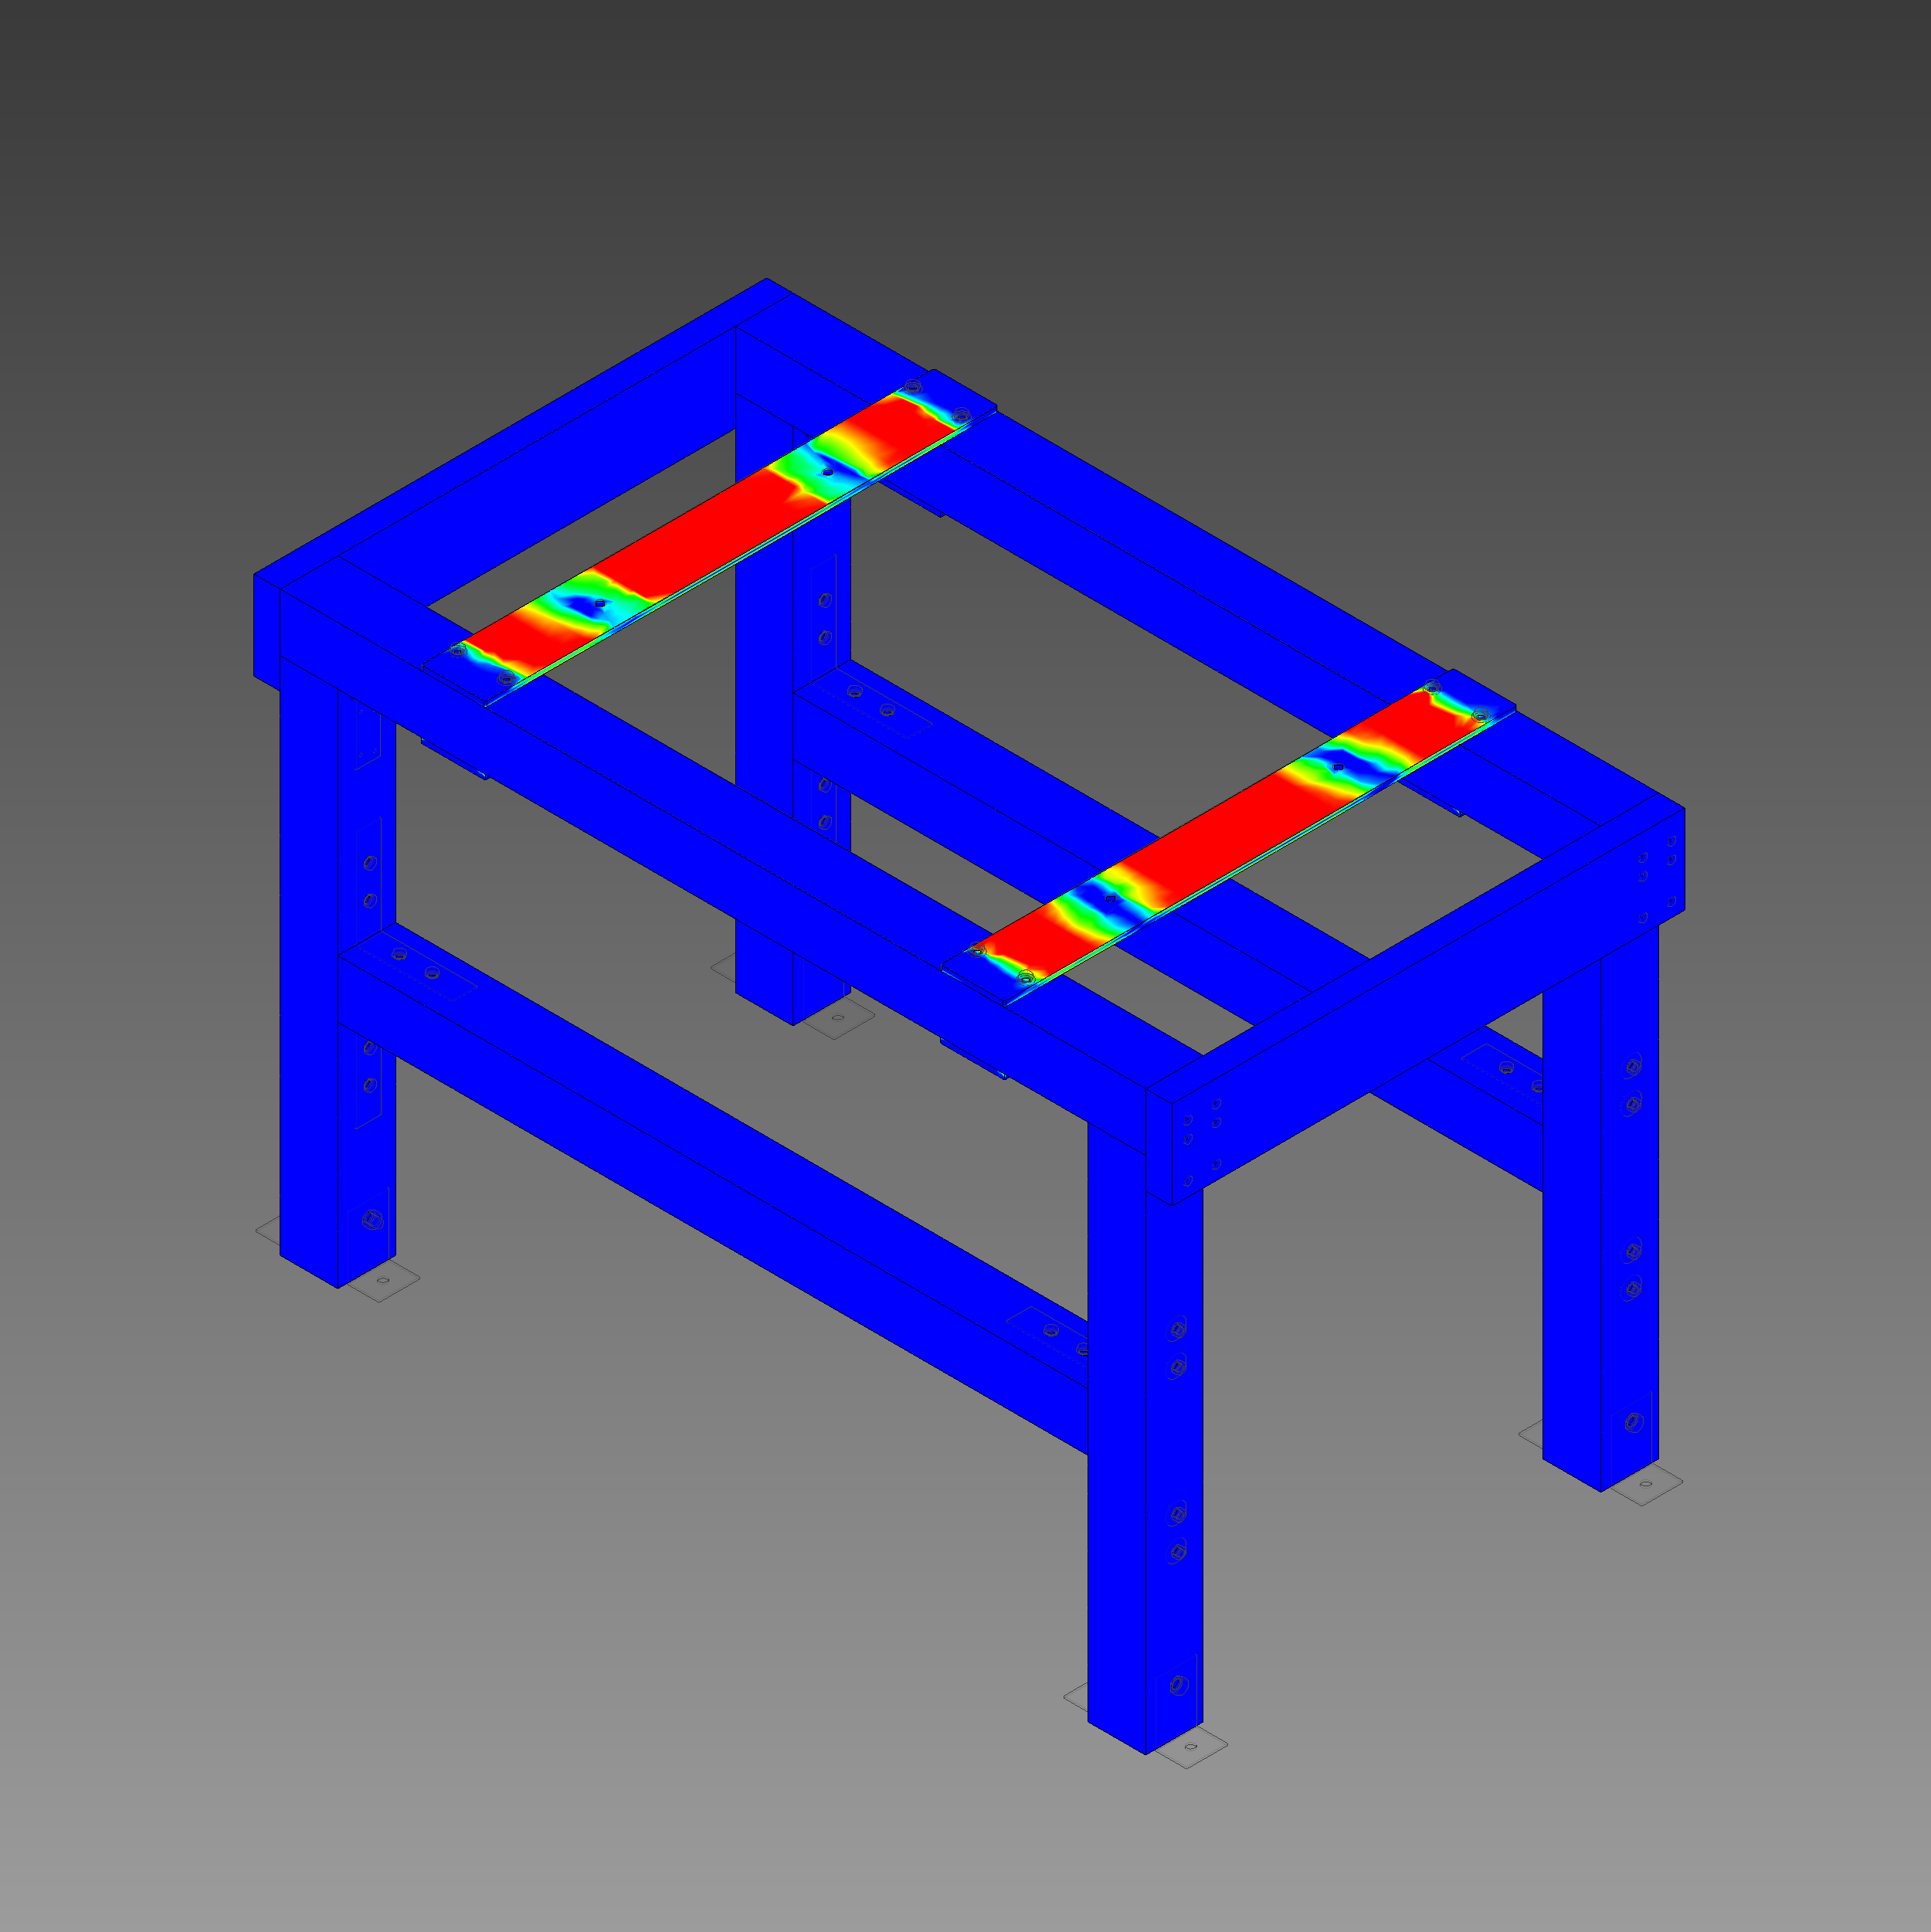
\includegraphics[width=1\linewidth]{Imagenes/rmesa_gen.png}
		\caption{}\label{fig:rmesa_gen}
	\end{subfigure}%
	\begin{subfigure}{0.49\linewidth}
		\centering
		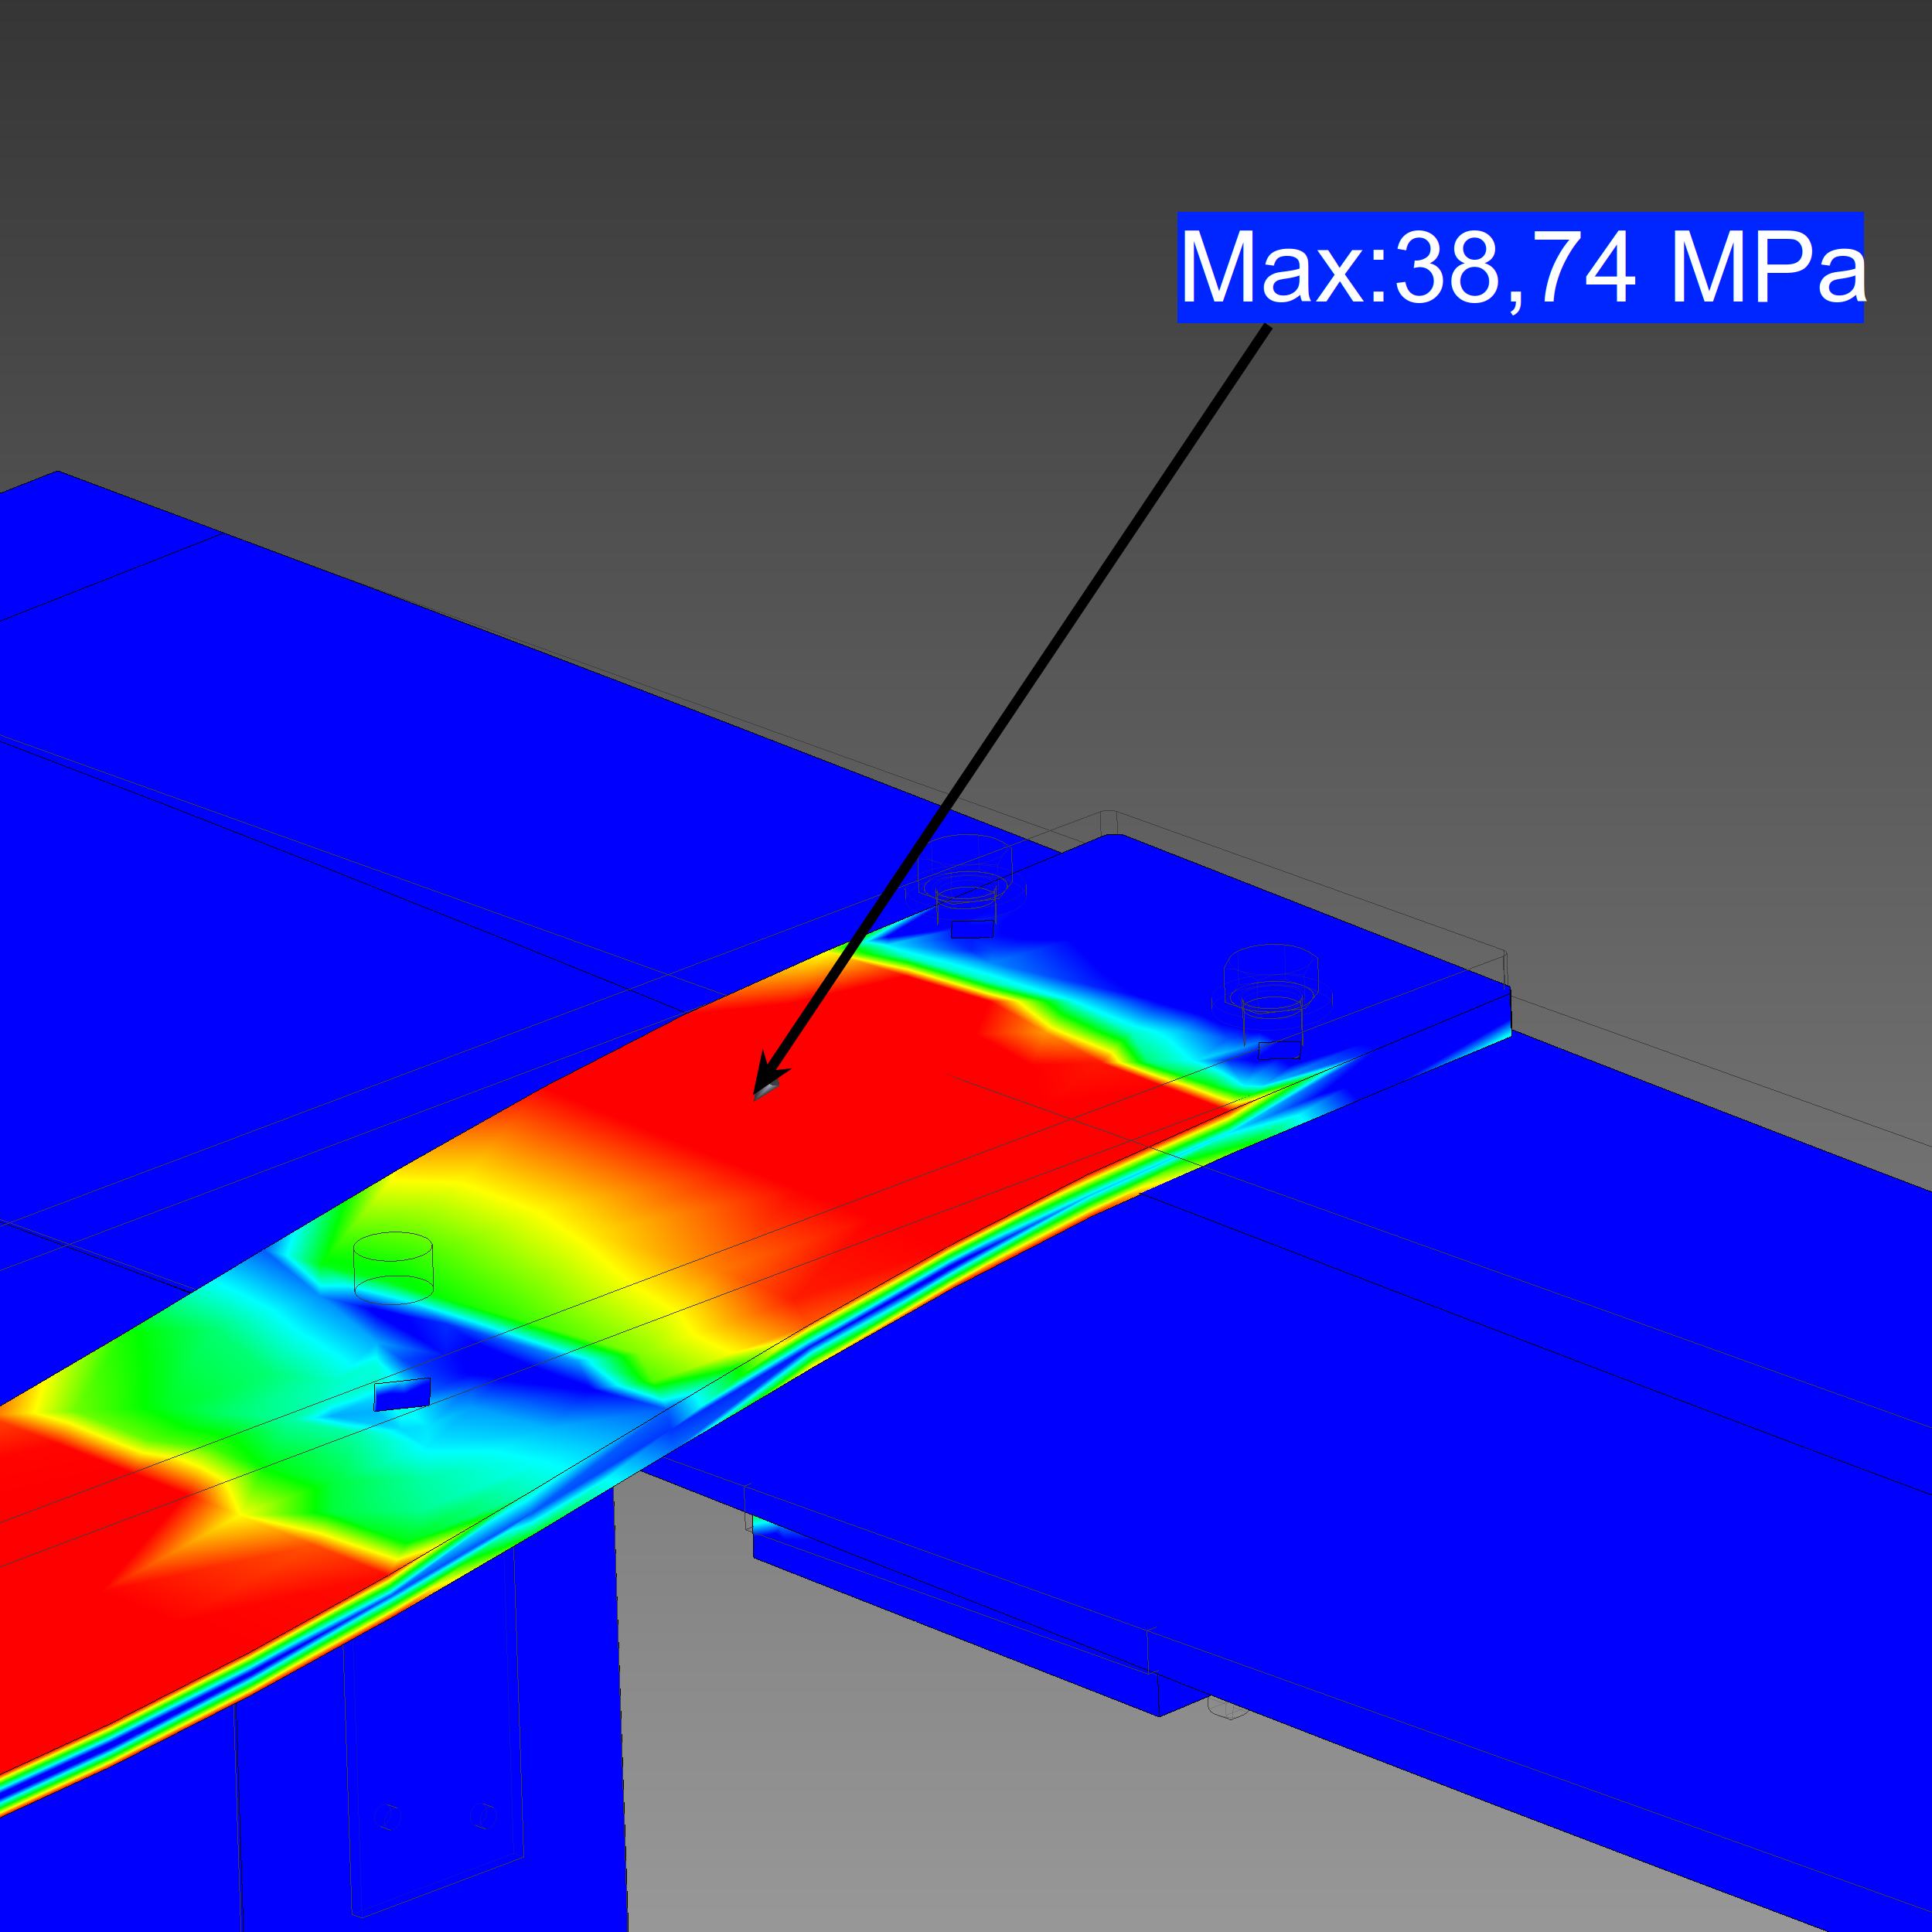
\includegraphics[width=1\linewidth]{Imagenes/rmesa_det.png}
		\caption{}\label{fig:rmesa_det}
	\end{subfigure}
\caption{La imagen (a) muestra los esfuerzos provocados por la mesa de fatiga sobre la estructura. La imagen (b) es un detalle del esfuerzo máximo, que se produce en los extremos de la pletina de acero.}
\label{fig:resultados_mesa}
\end{figure}

En definitiva, tanto los resultados obtenidos por la simulación como los obtenidos a través en base al cálculo y la norma de madera, nos indican que la madera no tendrá problemas en soportar la carga estática de la máquina por su sobredimensionamiento. Se confirman los puntos críticos del diseño general y, por último, los resultados del análisis modal revelan que no habrán problemas con la frecuencia natural de la estructura y el funcionamiento de la máquina de fatiga.

\section{Modelo del sistema}

\subsection{Comportamiento del modelo}
Con la caracterización y el levantamiento de información de los distintos componentes, junto a la elección de $c_1$, $c_2$ y de las variables de la función $\phi$, nos permite resolver y obtener valores del movimiento lineal, angular y la carga a la que está sometida la probeta. El tiempo de integración para cada una de las soluciones será entre 0 y 10 segundos. Se utilizará una tolerancia relativa y absoluta de $10^{-8}$. En consecuencia, al resolver el sistema de ecuaciones \ref{eq:mov_matriz} a través de los códigos de la sección \ref{sec:sol_part}, se obtiene la posición ($y,\theta$) y la velocidad ($\dot{y},\dot{\theta}$) del brazo de carga respecto a su centro de masa. Las imágenes \ref{fig:yt_2} y \ref{fig:ytp_2} muestran las curvas de cada coordenada.

Utilizando la ecuación \ref{eq:fuerza_probeta} para cada valor de $y_2(t)$, se obtiene la carga aplicada sobre la probeta $F(t)$ a lo largo del tiempo. La figura \ref{fig:f_2} muestra la curva de esta fuerza para la misma configuración de las imágenes anteriores.  

En este conjunto de imágenes se aprecia como el sistema tiene dos etapas principales: (a) la estabilización y reposo del sistema y (b) el inicio de la función $\phi$. (a) La primera etapa comienza en $t=0$, cuando se encuentra en un estado inicial $(y, \dot{y}, \theta, \dot{\theta}) = (0,0,0,0)$. Tanto la probeta y las barras en voladizo se encuentran sólo bajo la acción de la gravedad, por lo tanto caen y comienzan a oscilar en torno a su posición de reposo, sin embargo, este movimiento decae a medida que avanza el tiempo producto de los amortiguadores. La velocidad de decaimiento de la vibración inicial está determinado por el valor de $c_1$ y $c_2$, teniendo un comportamiento subamortiguado. (b) A continuación, desde el segundo 2 la función $\phi$ comienza a acelerar suavemente hasta llegar a la velocidad $\omega_{max} = 25$ [rad/s], punto en el cual la vibración es constante y estable en el tiempo. A partir de este punto, se extraen la información respectiva de la fuerza máxima, media y alternante, utilizando las ecuaciones \ref{eq:f_max}, \ref{eq:f_m} y \ref{eq:f_a}. 

\begin{figure}[h]
\centering
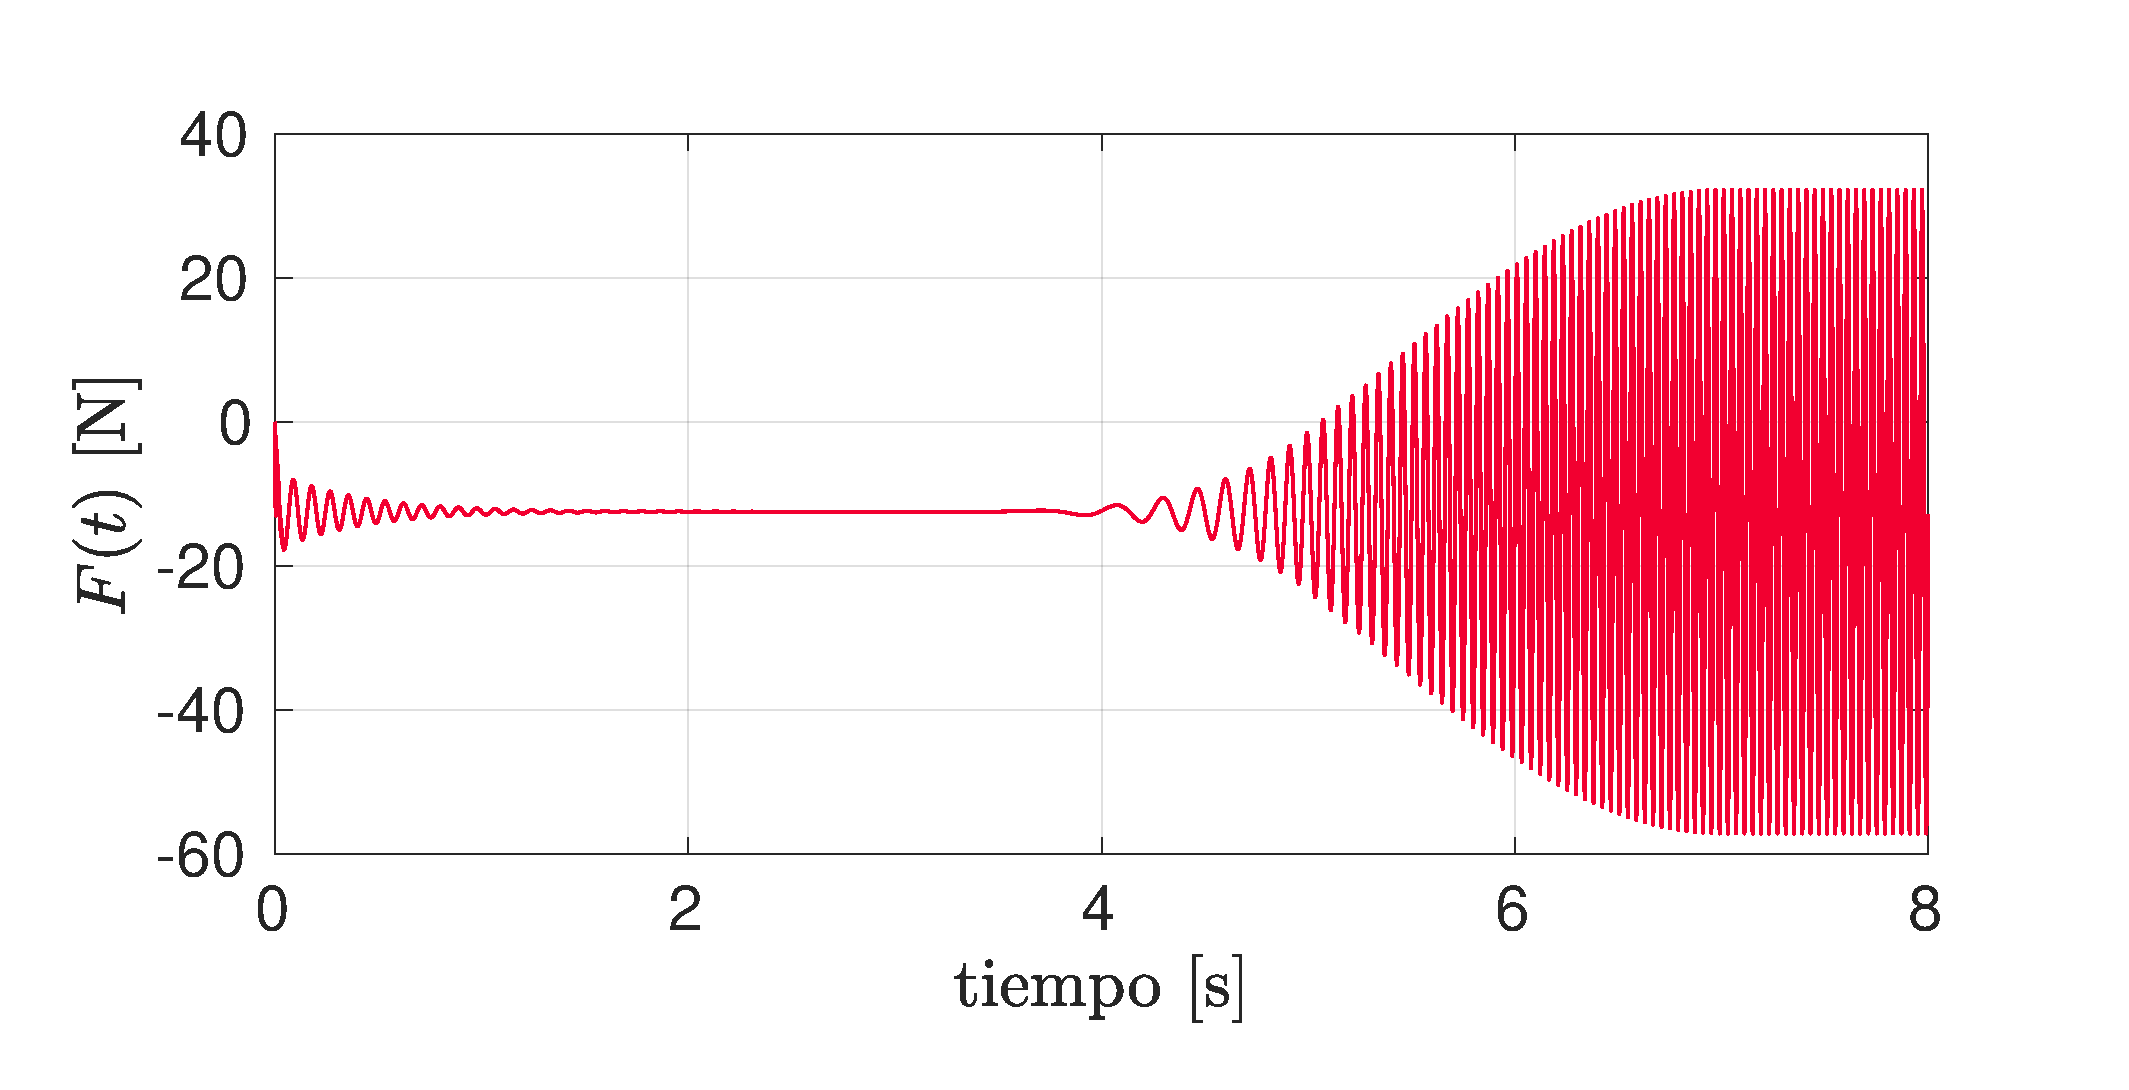
\includegraphics[width=0.95\linewidth, trim={0cm 1cm 2cm 1cm},clip]{Imagenes/f_2.pdf}
\caption{Fuerza aplicada sobre la probeta $F(t)$ en el tiempo.}
\label{fig:f_2}
\end{figure}

\begin{figure}[p]
\centering
	\begin{subfigure}{1\linewidth}
		\centering
		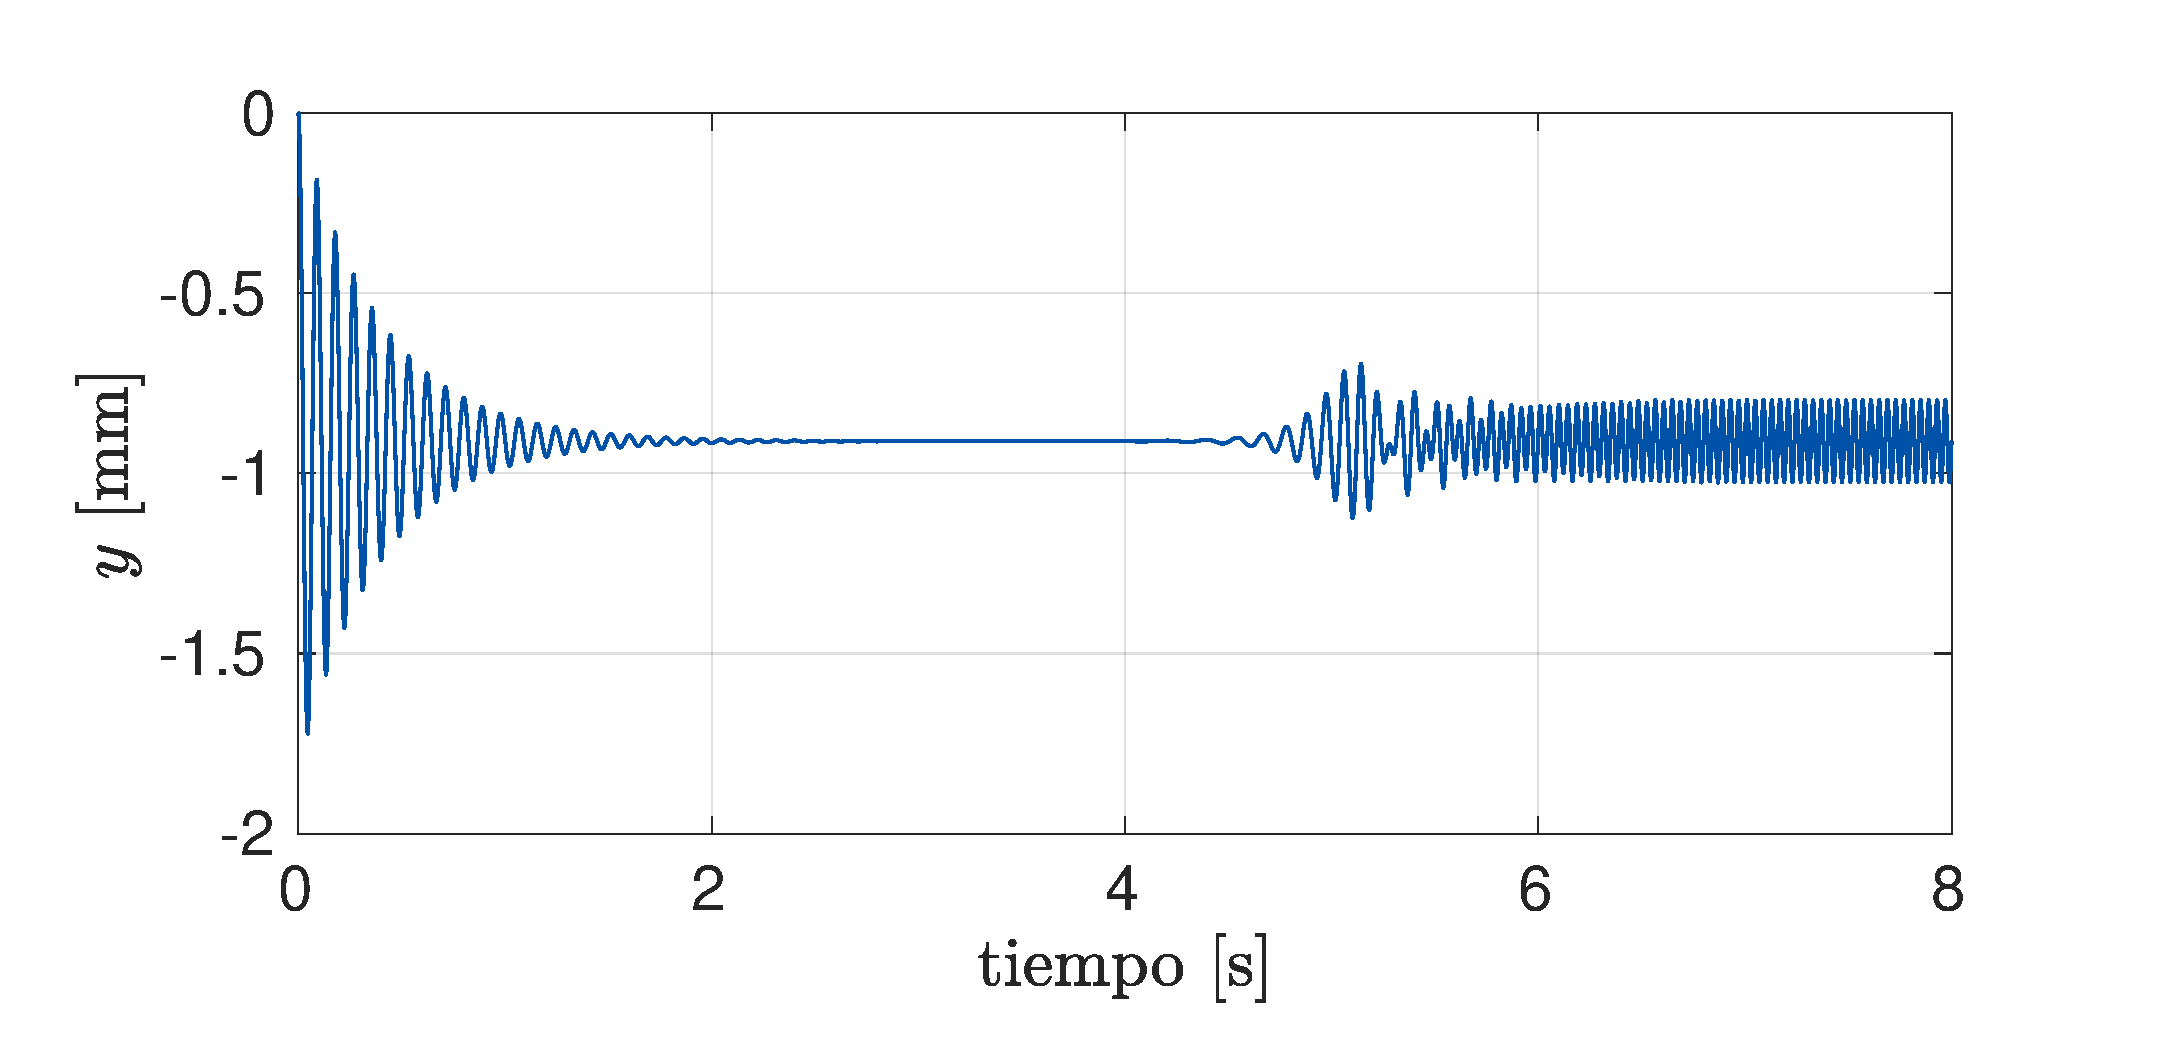
\includegraphics[width=1\linewidth]{Imagenes/y_2.pdf}
		\caption{}\label{fig:y_2}
	\end{subfigure}
	\begin{subfigure}{1\linewidth}
		\centering
		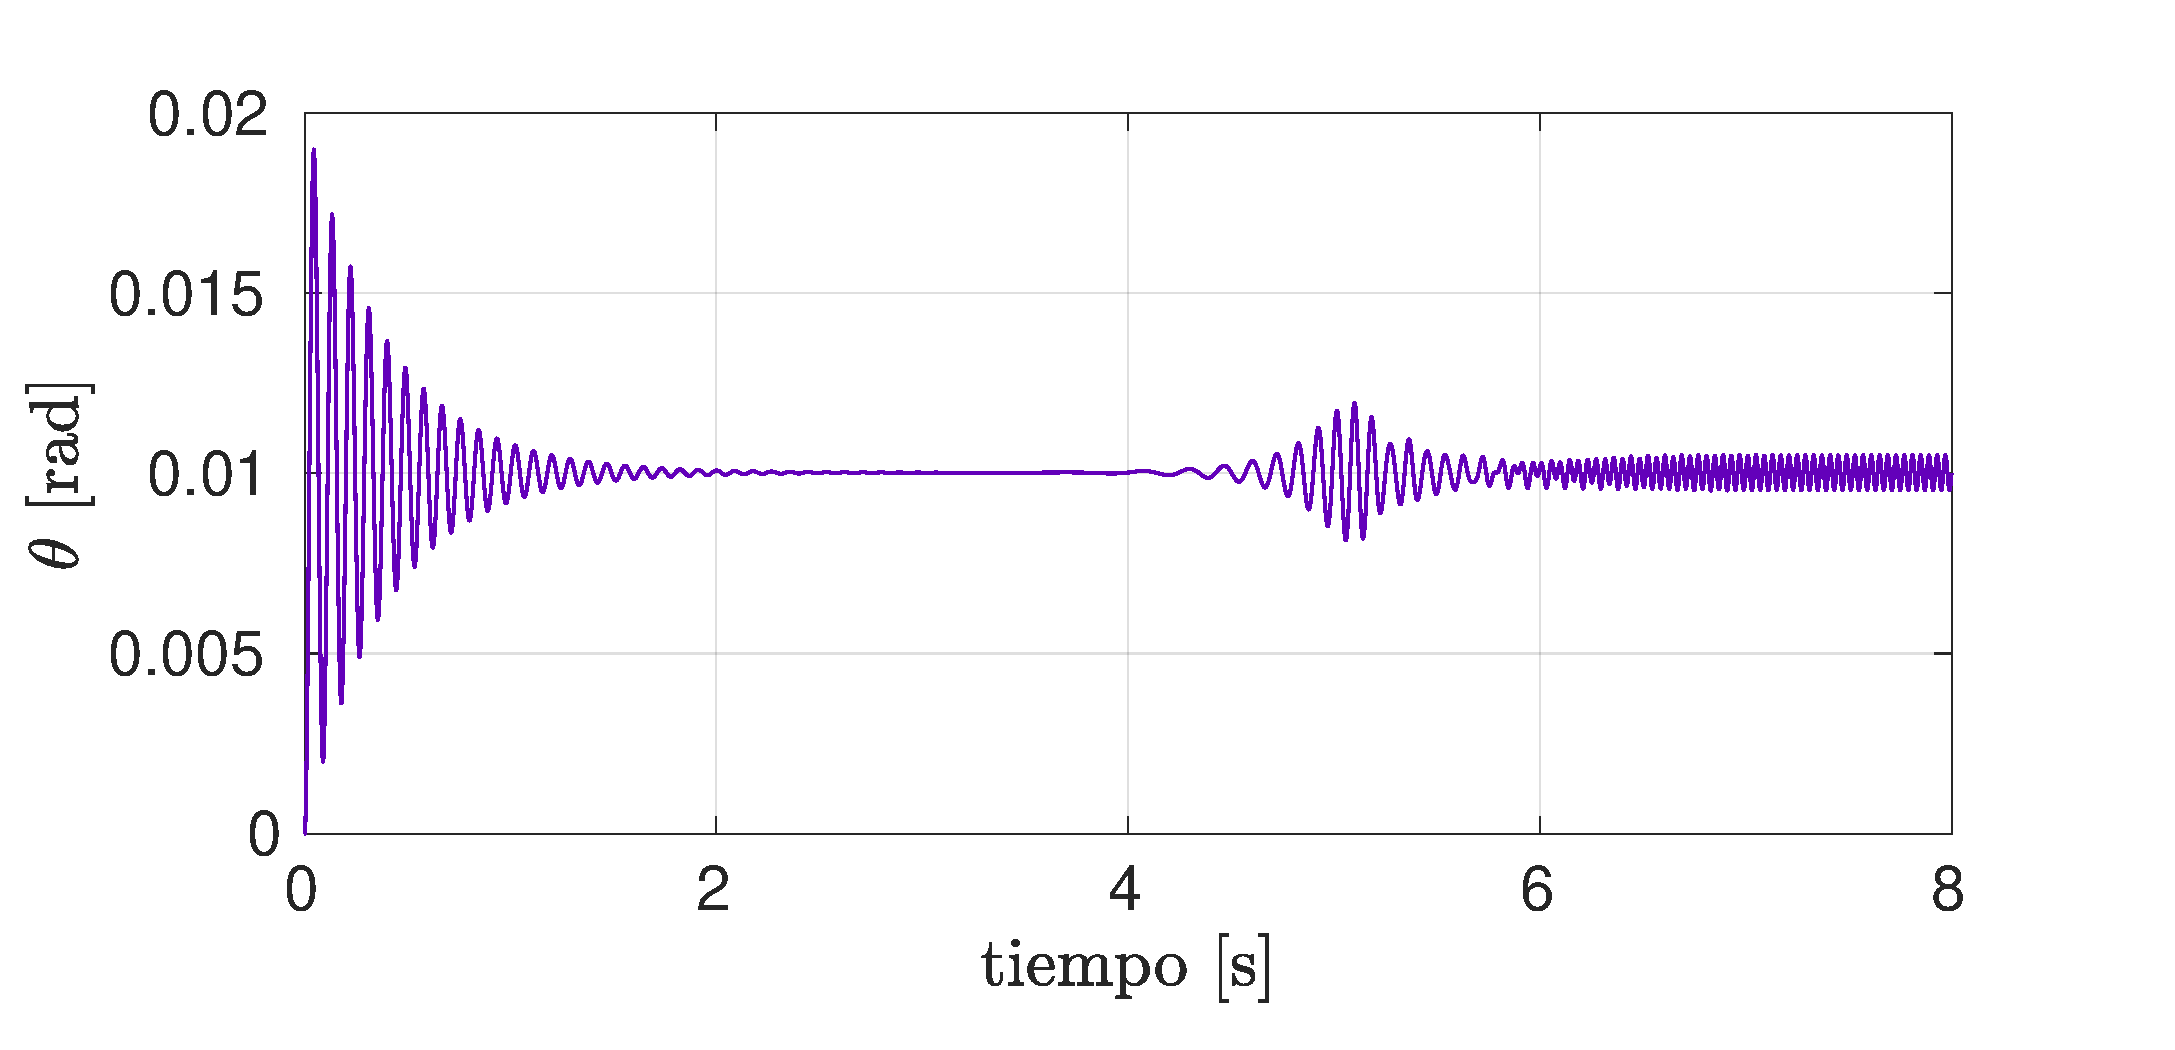
\includegraphics[width=1\linewidth]{Imagenes/t_2.pdf}
		\caption{}\label{fig:t_2}
	\end{subfigure}
\par\bigskip
\caption{Desplazamiento en el tiempo respecto al eje $y$ (a) y $\theta$ (b) del centro de masa del brazo de carga.}
\label{fig:yt_2}
\end{figure}


\begin{figure}[p]
\centering
	\begin{subfigure}{1\linewidth}
		\centering
		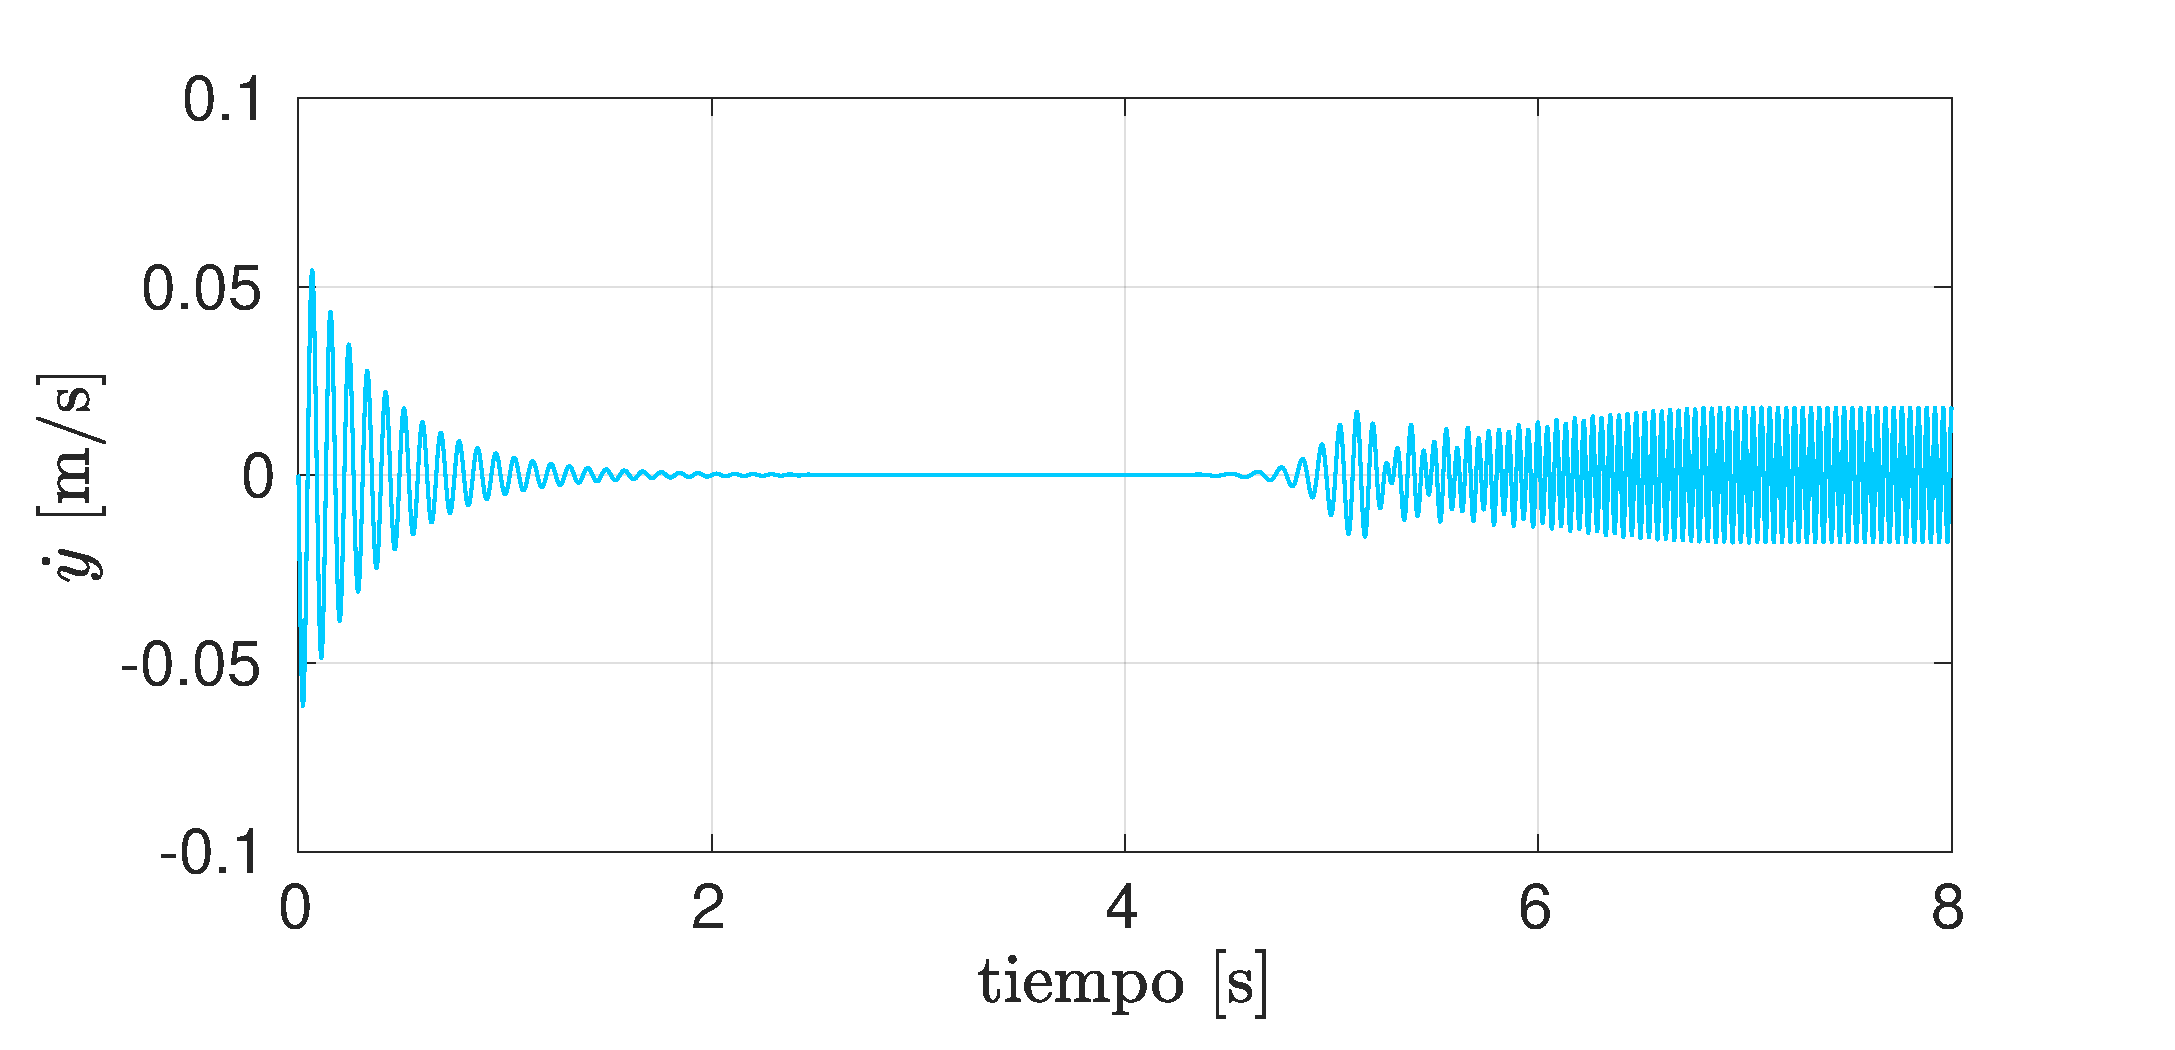
\includegraphics[width=1\linewidth]{Imagenes/yp_2.pdf}
		\caption{}\label{fig:yp_2}
	\end{subfigure}
	\begin{subfigure}{1\linewidth}
		\centering
		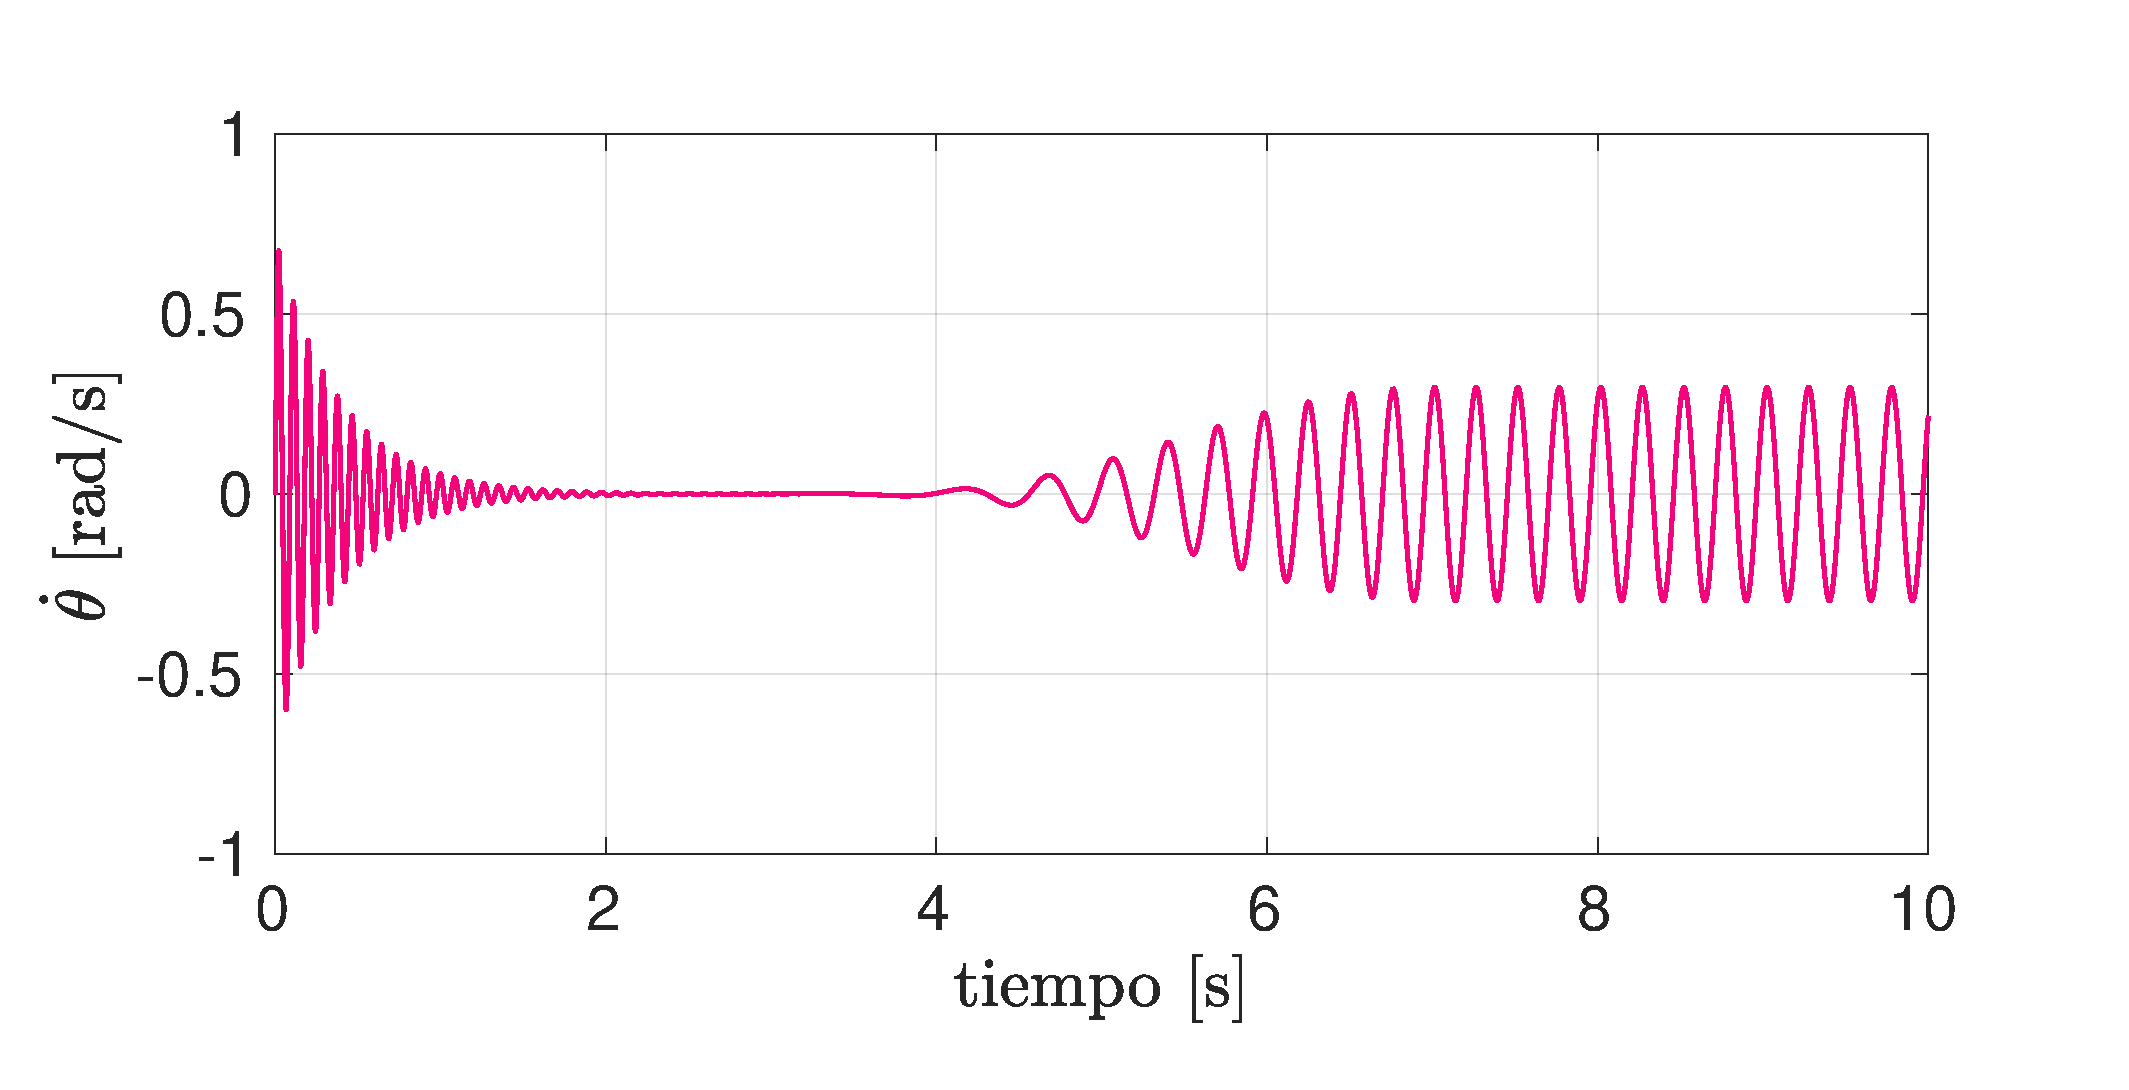
\includegraphics[width=1\linewidth]{Imagenes/tp_2.pdf}
		\caption{}\label{fig:tp_2}
	\end{subfigure}
\par\bigskip
\caption{Velocidad respecto la tiempo en el eje $y$ (a) y rotacional (b) del centro de masa del brazo de carga.}
\label{fig:ytp_2}
\end{figure}

%\begin{figure}[h]
%\centering
%	\begin{subfigure}{1\linewidth}
%		\centering
%		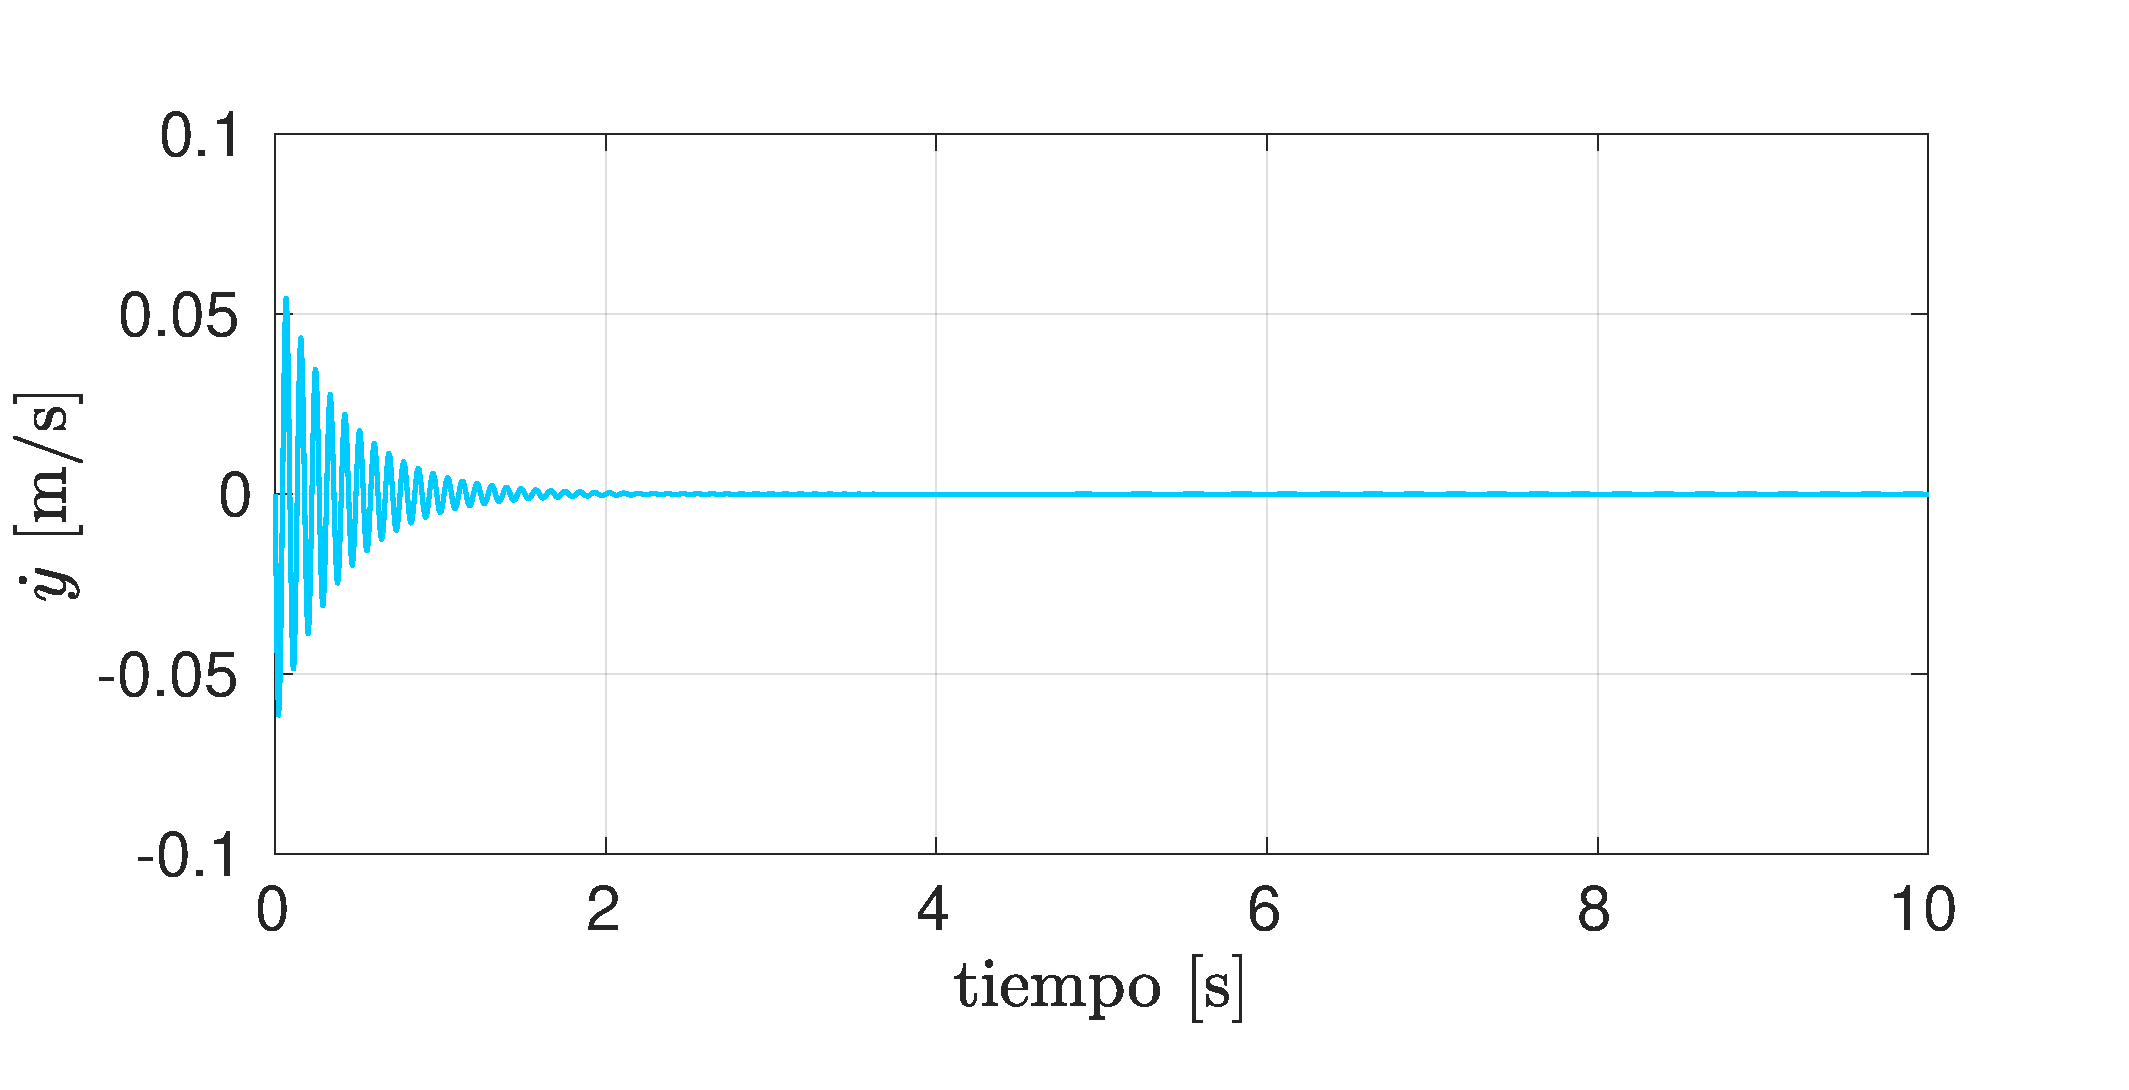
\includegraphics[width=1\linewidth]{Imagenes/yp_1.pdf}
%		\caption{}\label{fig:yp_1}
%	\end{subfigure}
%	\begin{subfigure}{1\linewidth}
%		\centering
%		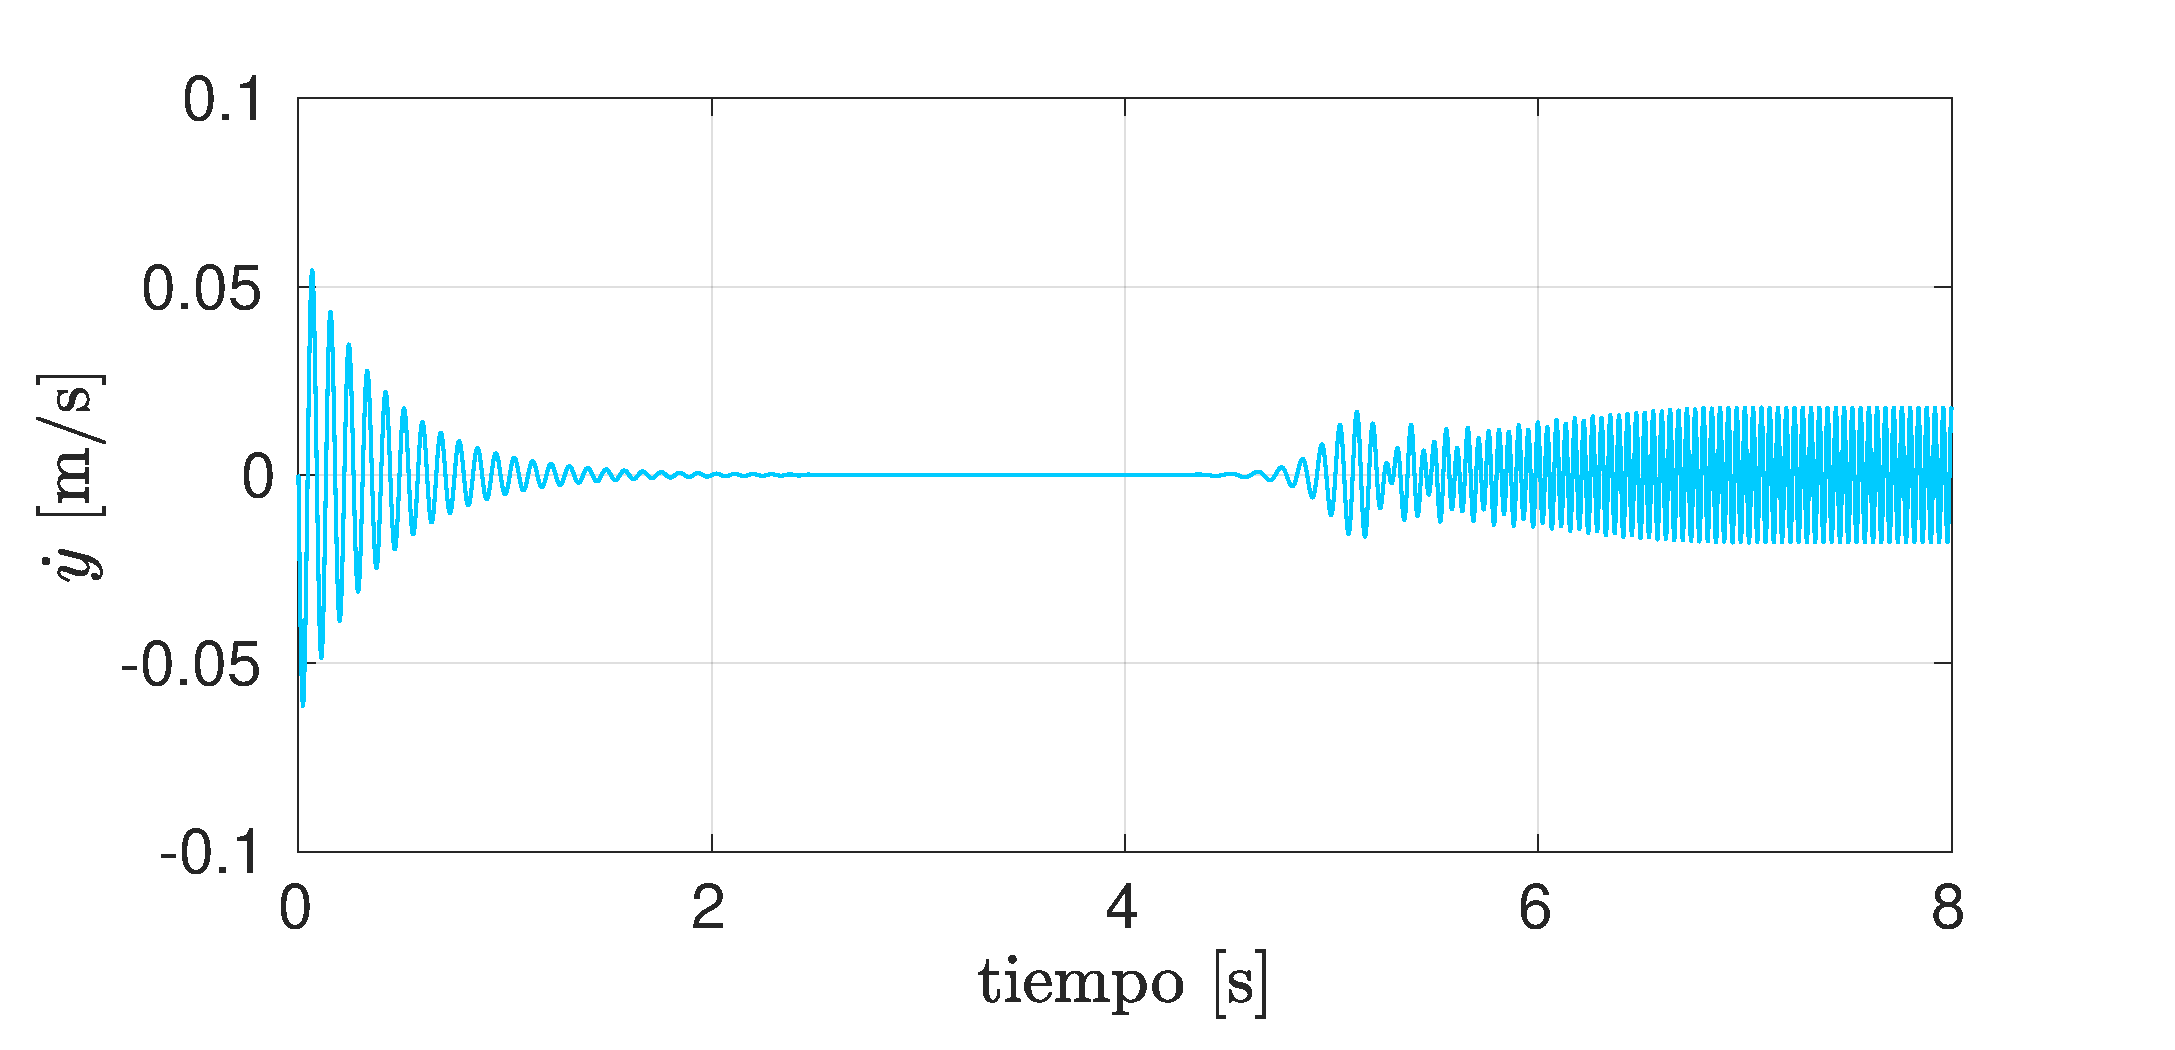
\includegraphics[width=1\linewidth]{Imagenes/yp_2.pdf}
%		\caption{}\label{fig:yp_2}
%	\end{subfigure}
%\par\bigskip
%\caption{sadfafssafdasf}
%\label{fig:vely_12}
%\end{figure}
%
%\begin{figure}[h]
%\centering
%	\begin{subfigure}{1\linewidth}
%		\centering
%		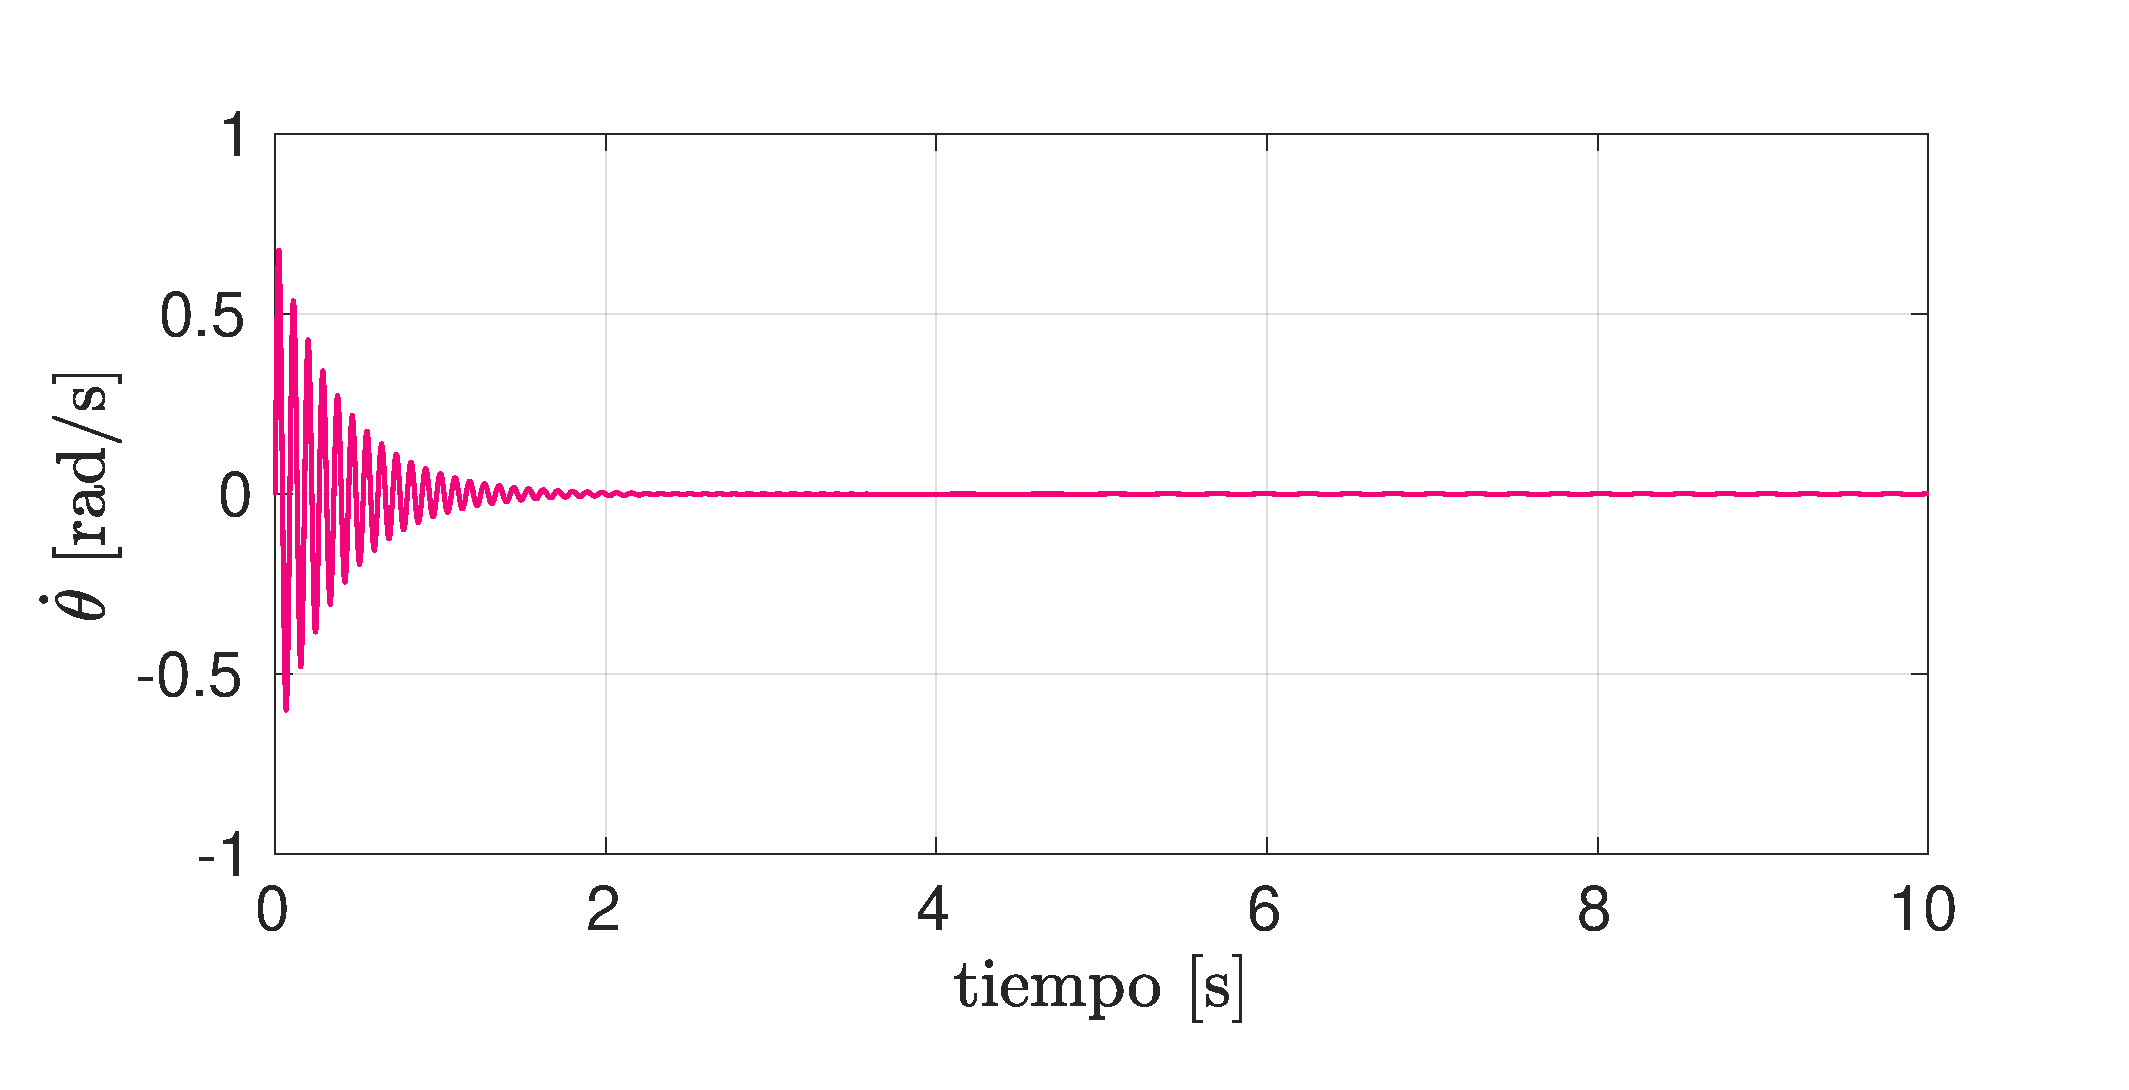
\includegraphics[width=1\linewidth]{Imagenes/tp_1.pdf}
%		\caption{}\label{fig:tp_1}
%	\end{subfigure}
%	\begin{subfigure}{1\linewidth}
%		\centering
%		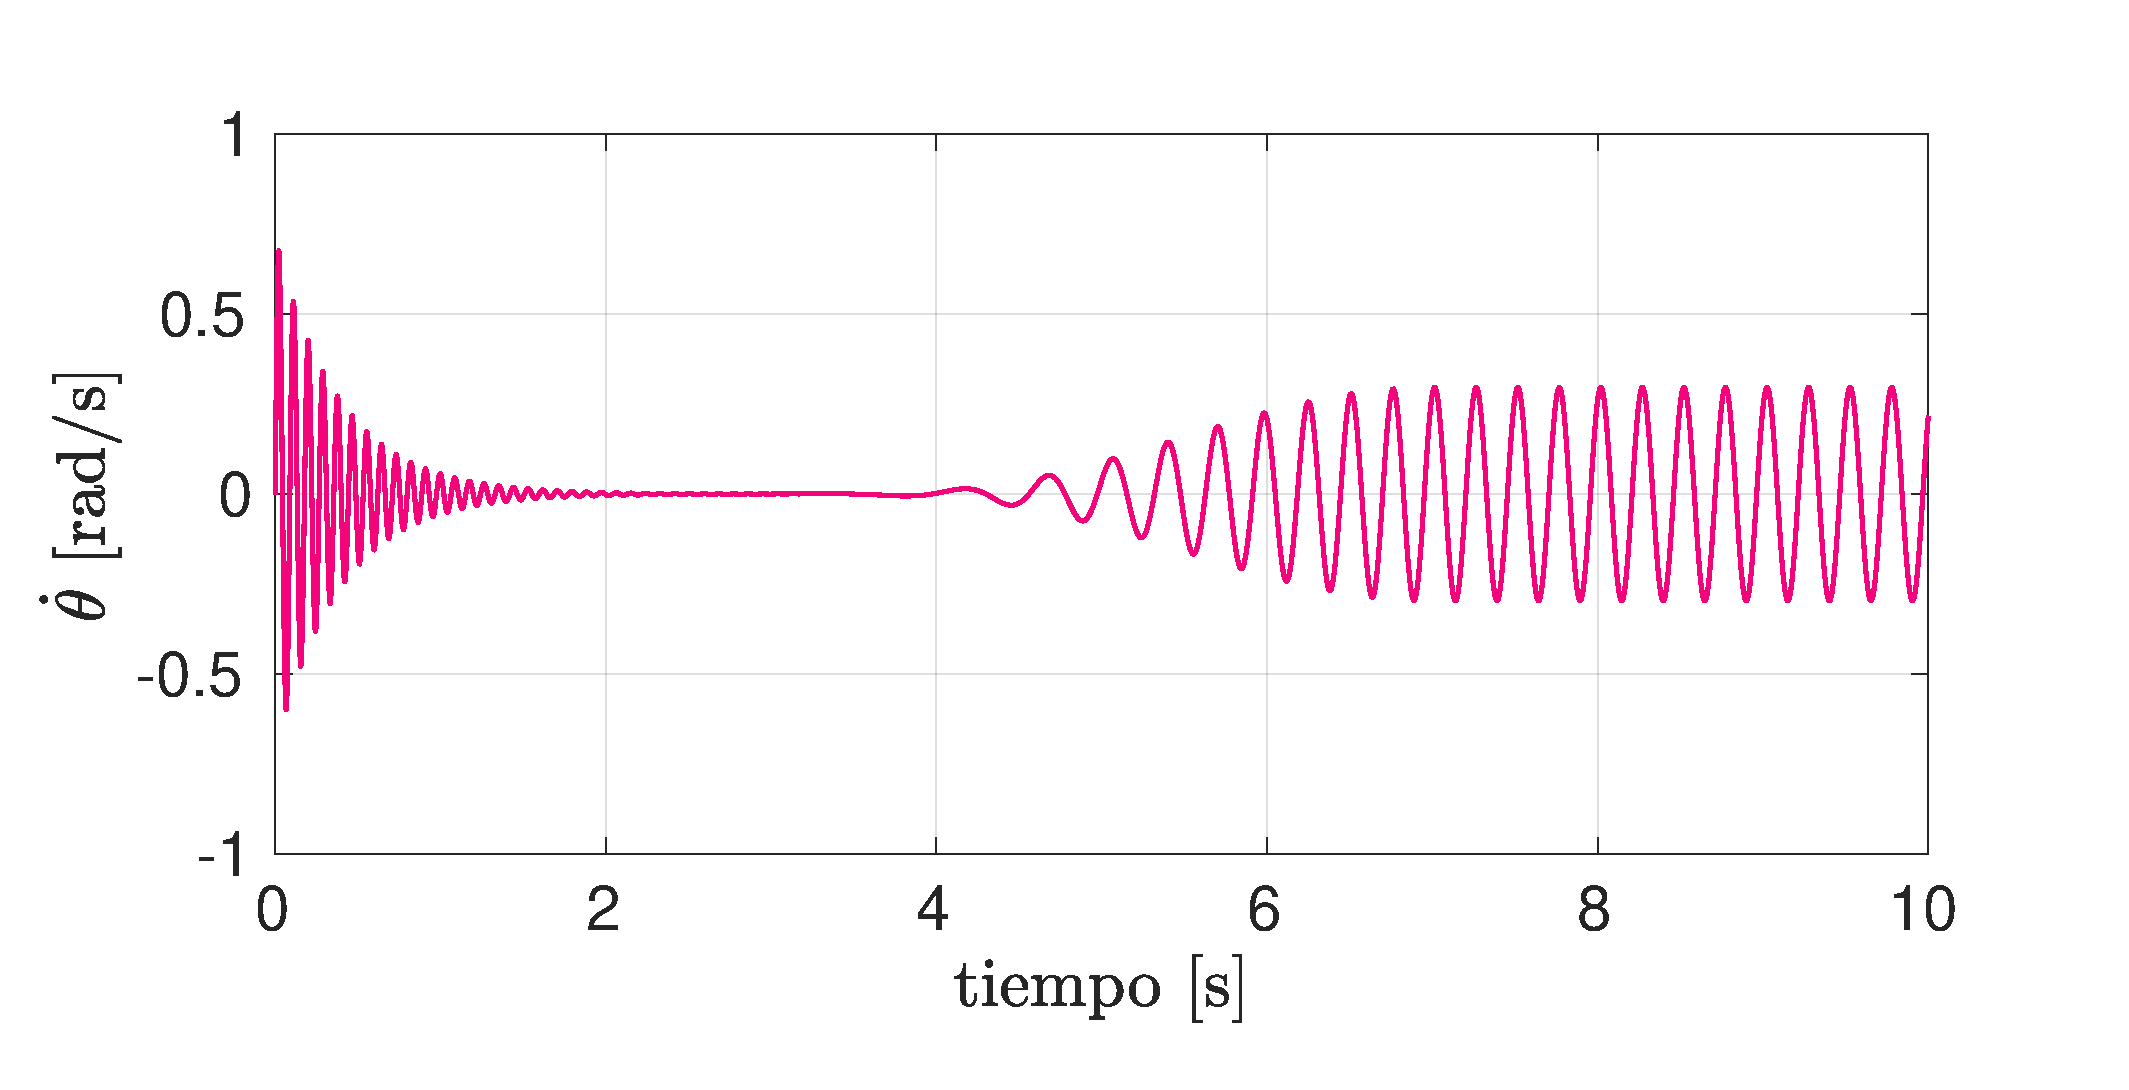
\includegraphics[width=1\linewidth]{Imagenes/tp_2.pdf}
%		\caption{}\label{fig:tp_2}
%	\end{subfigure}
%\par\bigskip
%\caption{sadfafssafdasf}
%\label{fig:velt_12}
%\end{figure}
 
\newpage
 
\subsection{Carga máxima y media para cada configuración} 

En la sección anterior, se mostraron los resultados y el comportamiento del modelo para una configuración en específico. En esta sección, a través del código de la sección \ref{sec:sol_gen}, se mostrarán los resultados de fuerza máxima y media para cada combinación de contrapesos expuesta en la tabla de carga. Al ordenar los resultados de la fuerza máxima con el mismo orden de la tabla de carga, es decir, respecto a $\Delta m$, se obtiene la curva que se muestra en la figura \ref{fig:fmax_dm}. A partir de la imagen, se puede establecer que no existe una relación entre la carga máxima $F_{max}$ y $\Delta m$ como sí lo estipula la tabla de carga. Por lo tanto, existe una diferencia sustancial entre la información entregada por la tabla de carga y lo que predice el modelo desarrollado en este trabajo. 

\begin{figure}[h]
\centering
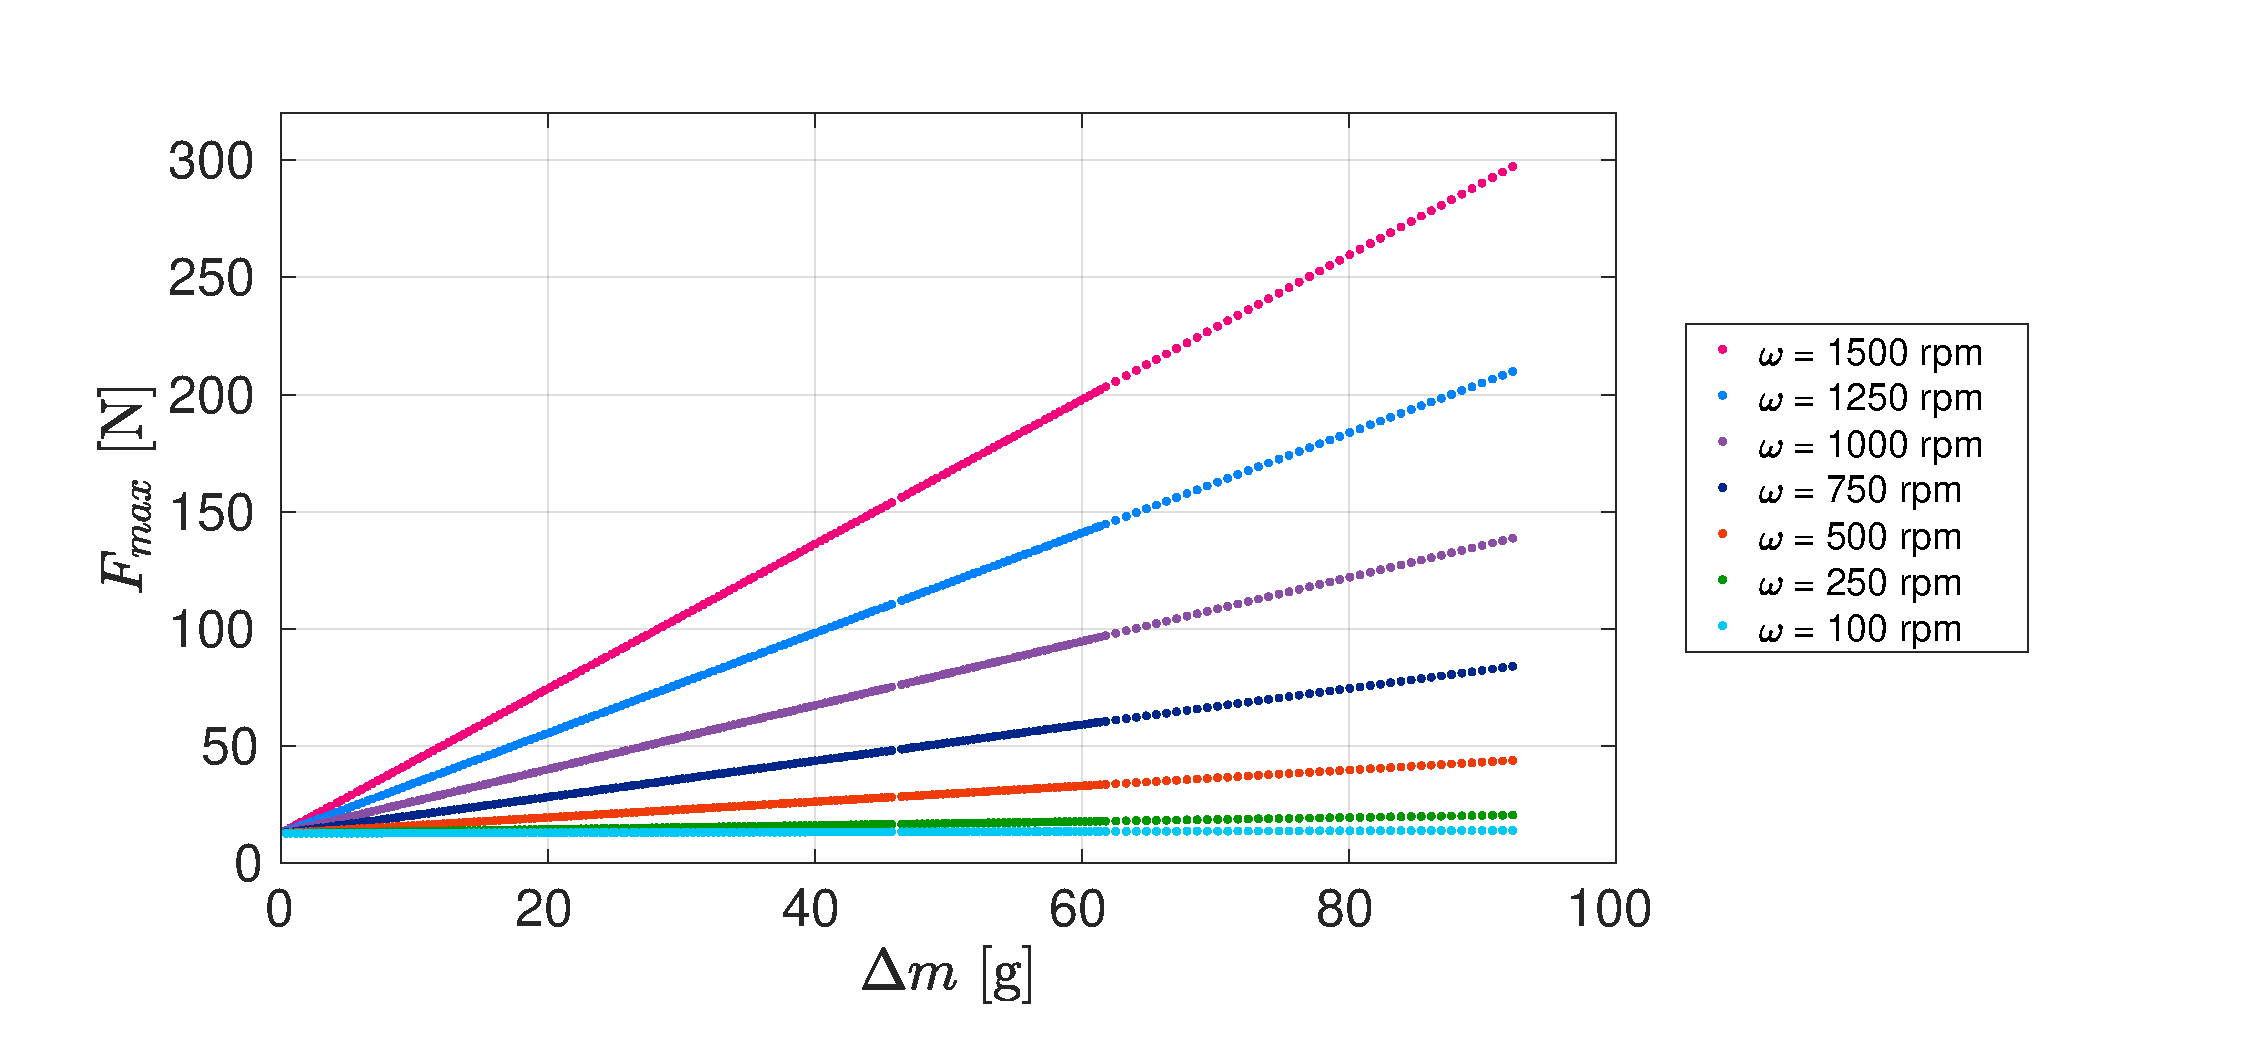
\includegraphics[width=\linewidth, trim={0cm 1cm 2cm 2cm},clip]{Imagenes/fmax_dm.pdf}
\caption{Distribución de la carga máxima $F_{max}$ versus la diferencia de masas $\Delta m$ de cada combinación de contrapesos.}
\label{fig:fmax_dm}
\end{figure}

En consecuencia, se propone tomar nuevamente $F_{max}$, pero ordenado respecto a la variable $\Psi = M_a \cdot e_{ga}$. Como resultado de esto, se obtiene la curva que se ve en la figura \ref{fig:fmax_psi}. En esta se puede ver que existe una relación entre ambas variables, por lo tanto, la carga máxima de cualquier combinación de contrapesos, a una velocidad $\omega_{max}$ constante, estará determinada por $\Psi$. En ese sentido, se puede definir la siguiente relación:
\begin{equation}\label{eq:func_psi}
	F(t) = f(\Psi)
\end{equation}
Así, la relación original que establece la tabla de carga, donde $F(t) = f(\Delta m)$, es contradictoria con los resultados del modelo de vibración propuesto. Si bien es necesario realizar un estudio que incluya mediciones de la máquina de fatiga para determinar la validez o el rechazo de las dos relaciones, cabe destacar que la única fuerza externa del sistema es provocada por el desequilibrio del motor, el cual, se define físicamente como $F_d(t) = \Psi \cdot (\dot{\phi}^2 \sin\phi - \ddot{\phi} \cos\phi)$. Es decir, en el desarrollo de este trabajo no se encontraron elementos que hagan pensar en $\Delta m$ como una variable fundamental que defina la obtención de la carga sobre la probeta.

\begin{figure}[]
\centering
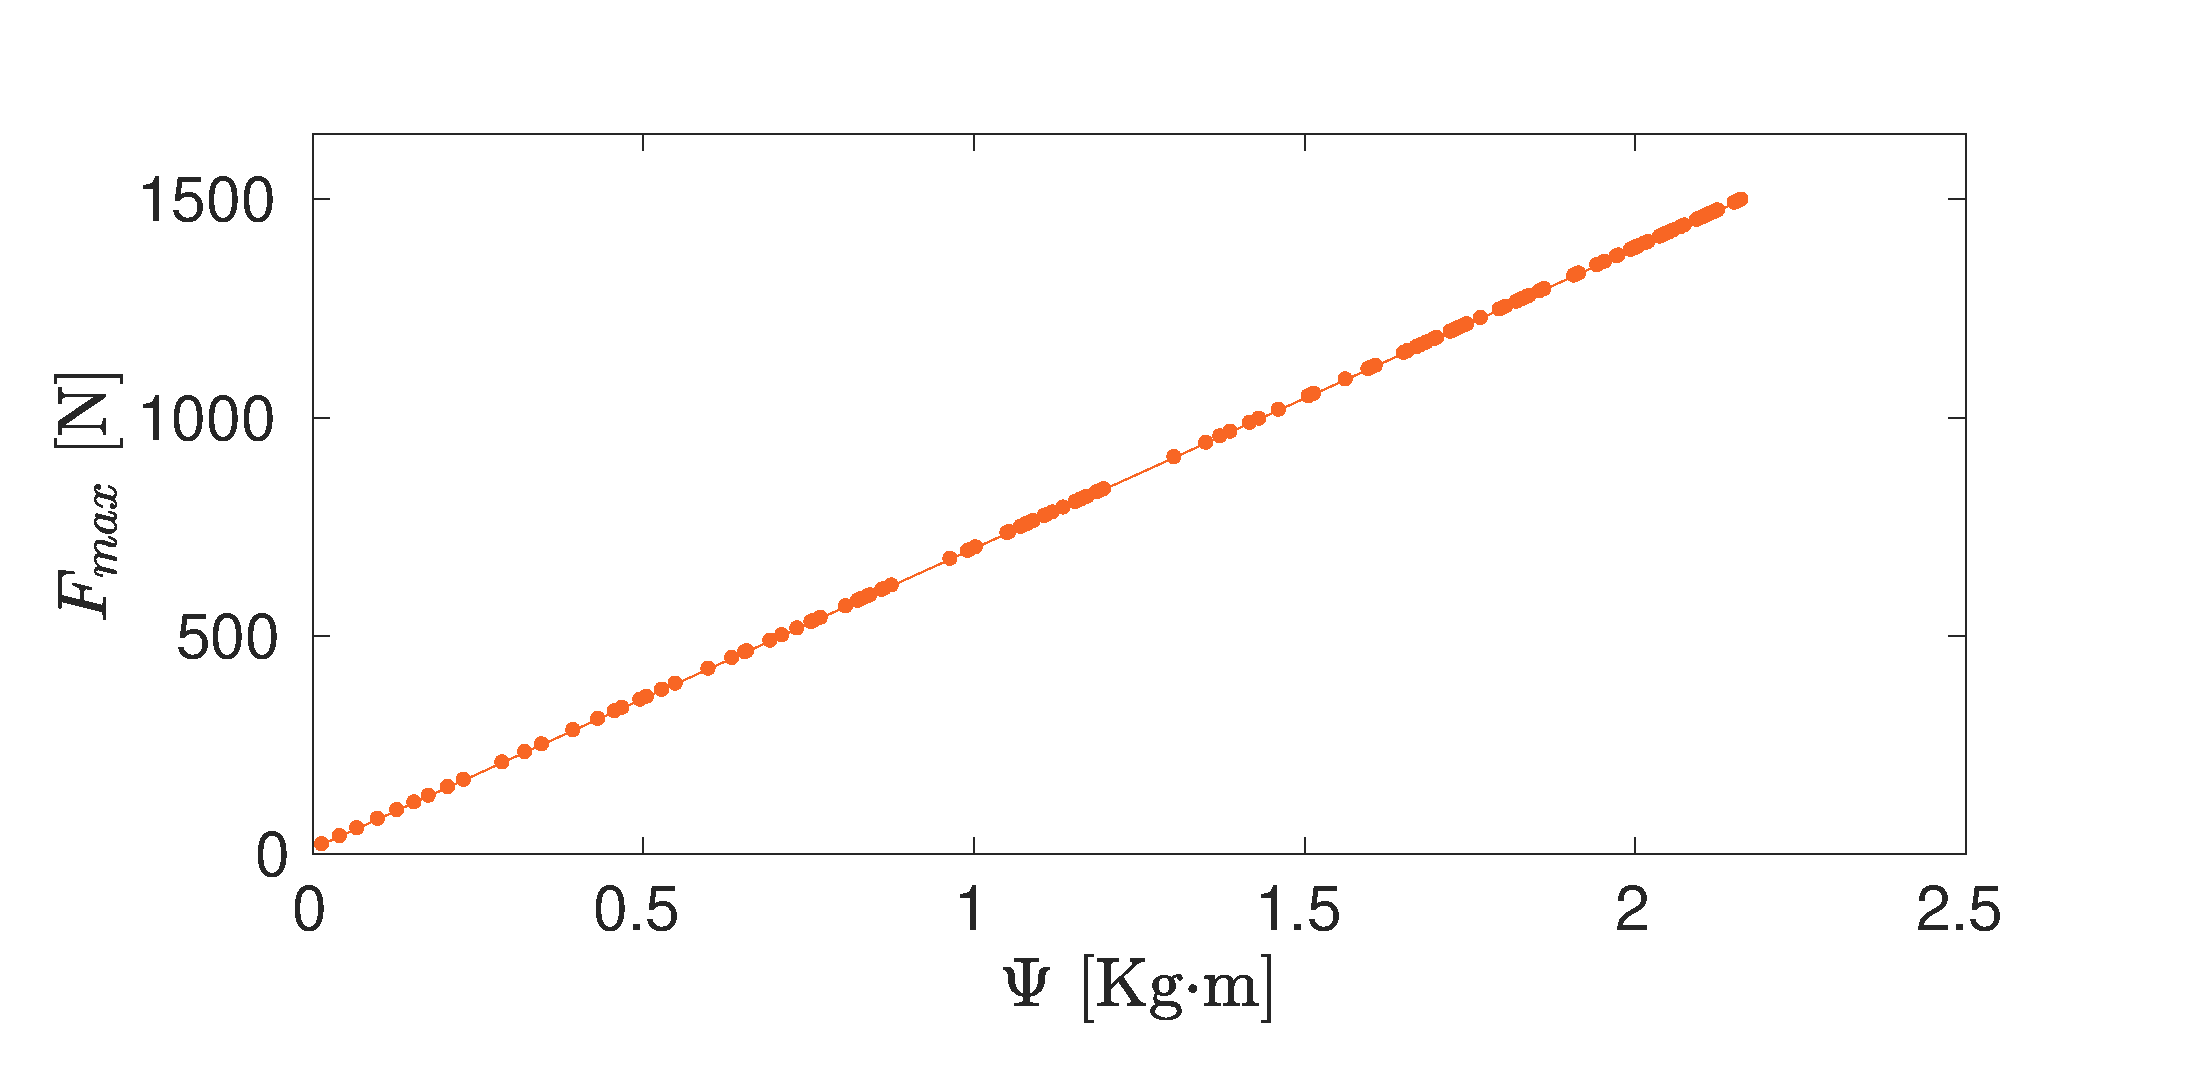
\includegraphics[width=\linewidth, trim={0cm 1cm 2cm 2cm},clip]{Imagenes/fmax_psi.pdf}
\caption{Curva de la carga máxima $F_{max}$ versus la variable $Psi$.}
\label{fig:fmax_psi}
\end{figure}
 
Por otro lado, la carga media tiene variaciones muy pequeñas, como se puede ver en la imagen \ref{fig:fm_dm}, siendo la diferencia máxima de $2.4\cdot10^{-4}$ [N]. Tomando en consideración que el orden de magnitud de las cargas máxima y alternantes está entre $10^1$ y $10^2$, dependiendo de la velocidad $\omega_{max}$, entonces se puede asumir que la carga media que sufrirá la probeta será constante y de una magnitud de $12.438$ [N]. 

\begin{figure}[]
\centering
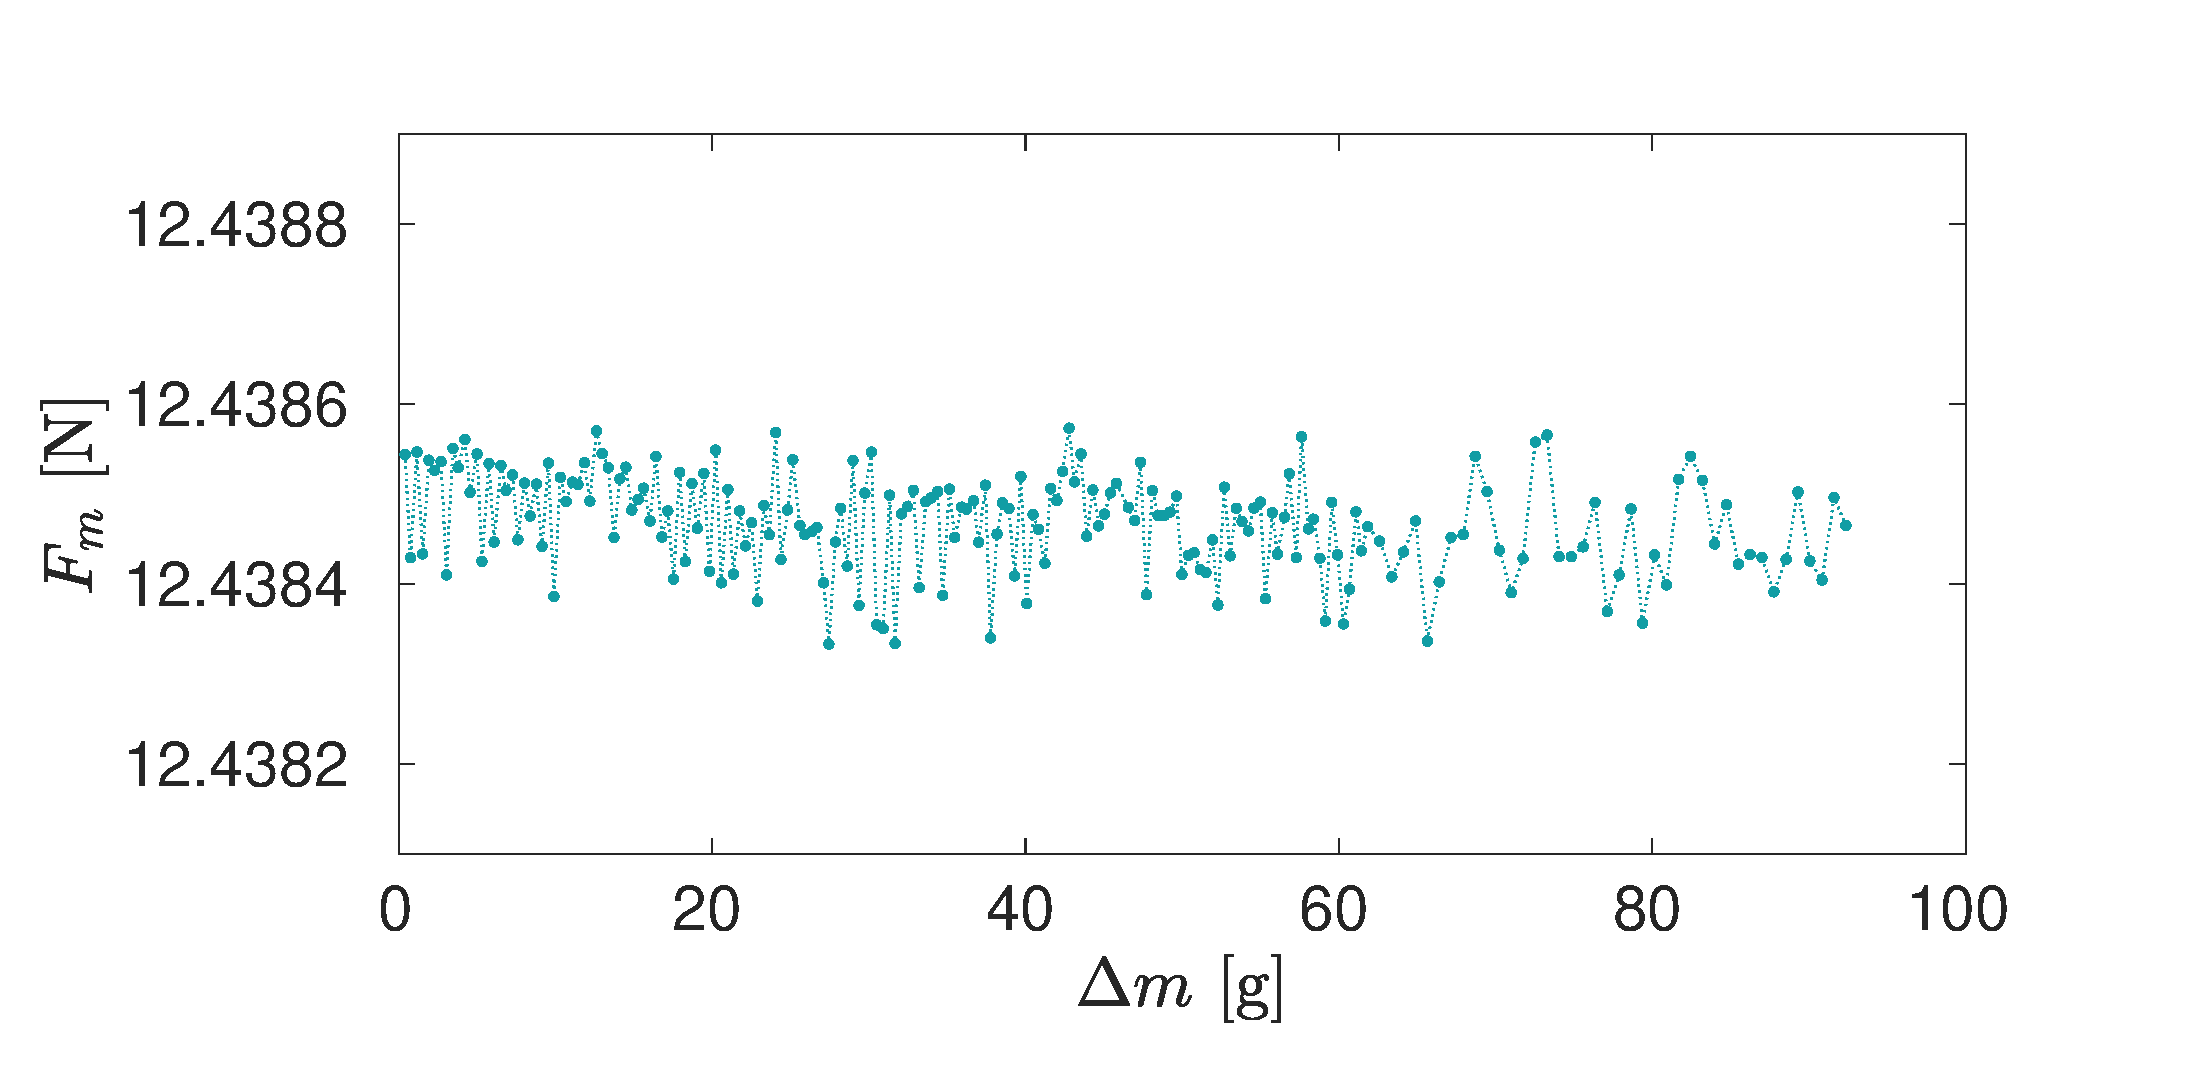
\includegraphics[width=\linewidth, trim={0cm 1cm 2cm 2cm},clip]{Imagenes/fm_dm.pdf}
\caption{sadfasdfsa}
\label{fig:fm_dm}
\end{figure}

\subsection{Influencia de la velocidad de rotación del disco desbalanceado sobre la carga en la probeta}

De manera análoga, se puede estudiar la influencia de la velocidad de giro máxima del disco desbalanceado sobre el movimiento del sistema. Las imágenes en \ref{fig:f_w520}, muestran $F(t)$ para dos velocidad distintas, $\omega_{max,a} = 5$ [rad/s] y $\omega_{max,b}=20$ [rad/s]. 

Ambas gráficas muestran no sólo como la frecuencia de la oscilación es menor en la imagen \ref{fig:f_w5} respecto a \ref{fig:f_w20}, como es esperable, sino que también la fuerza sobre la probeta aumenta en la medida que la velocidad de rotación del disco es mayor. Esta información, junto a la expuesta en la sección anterior, muestra que el modelo responde a las distintas variables de la fuerza provocada por el disco $F_d(t)$. 

\begin{figure}[p]
\centering
	\begin{subfigure}{1\linewidth}
		\centering
		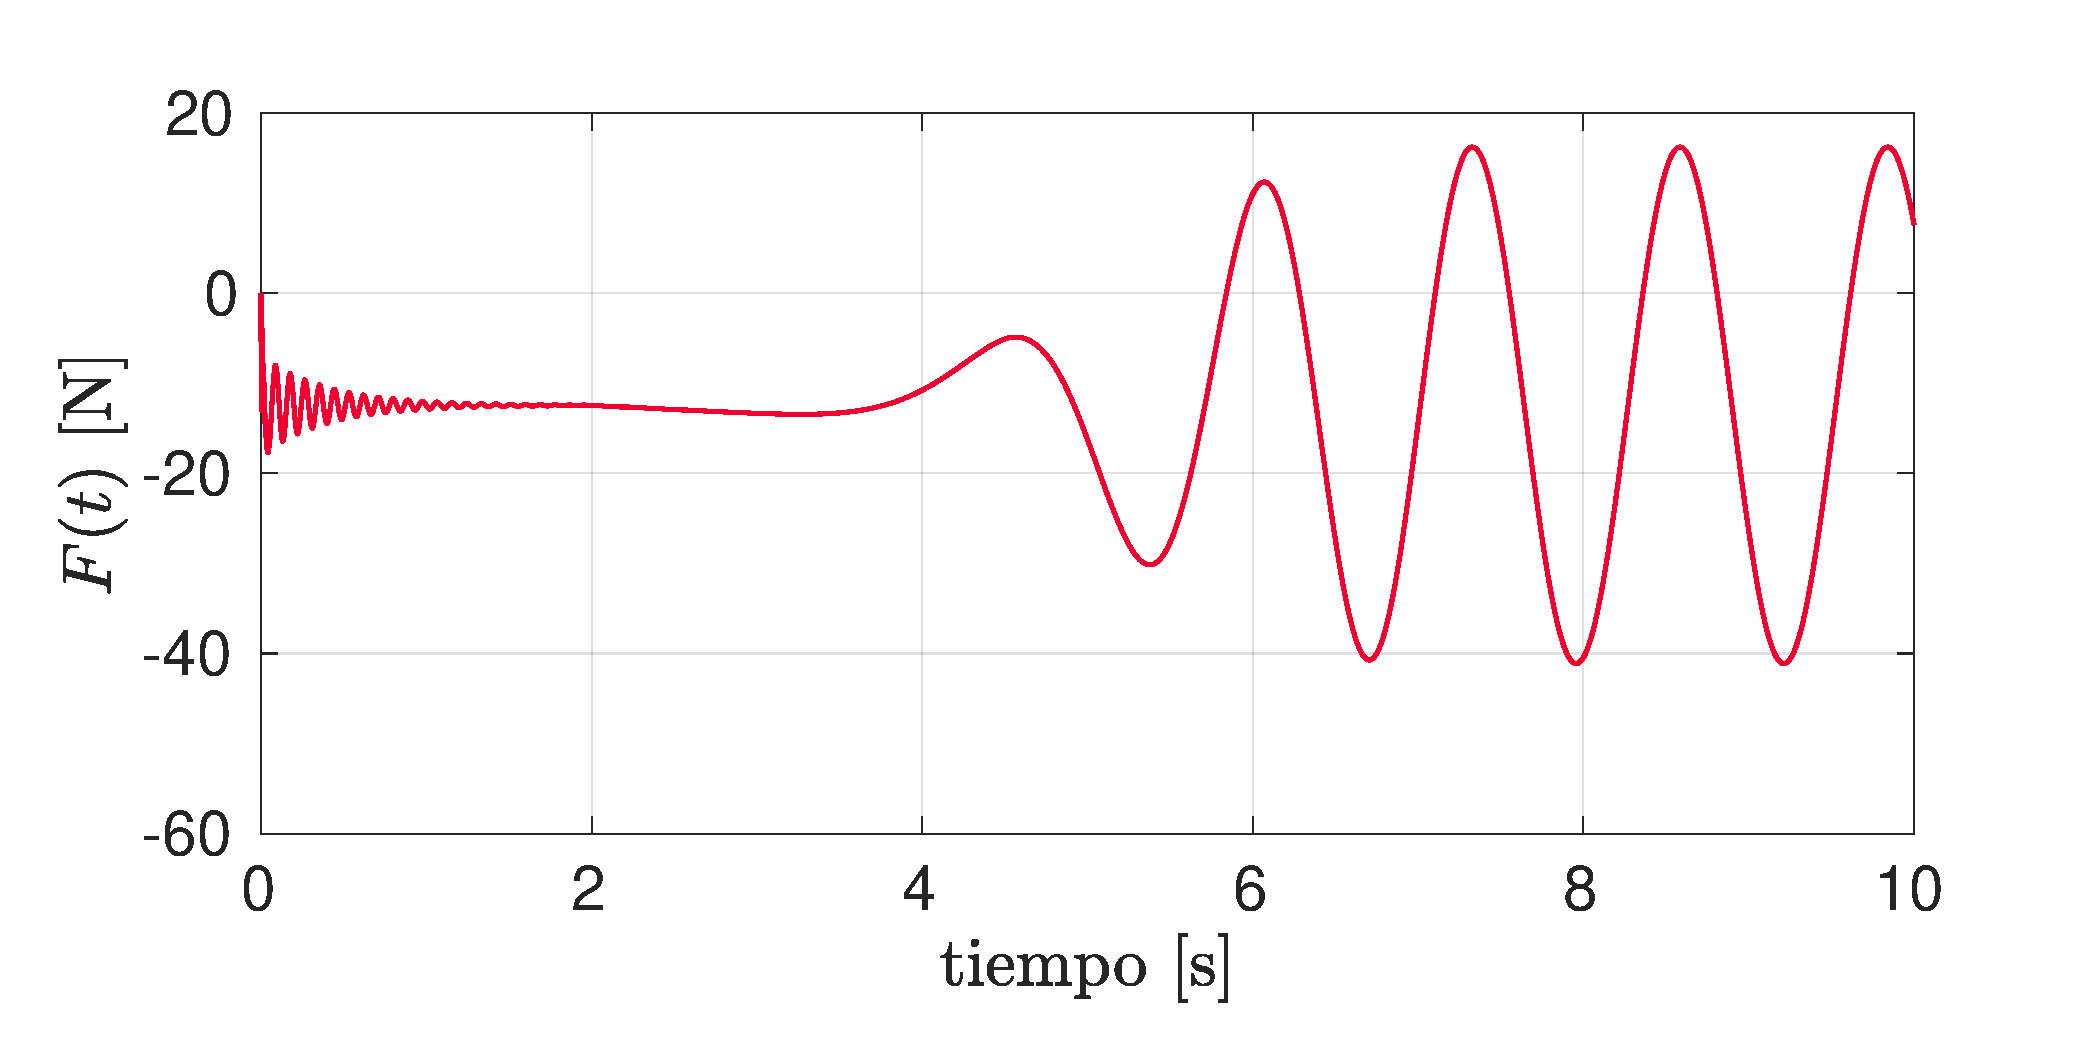
\includegraphics[width=\linewidth, trim={0cm 0cm 2cm 0cm},clip]{Imagenes/f_w5.pdf}
		\caption{Fuerza sobre la probeta a través del tiempo a $\,\omega_{max}=5$ [rad/s]}
		\label{fig:f_w5}
	\end{subfigure}
	\begin{subfigure}{1\linewidth}
		\centering
		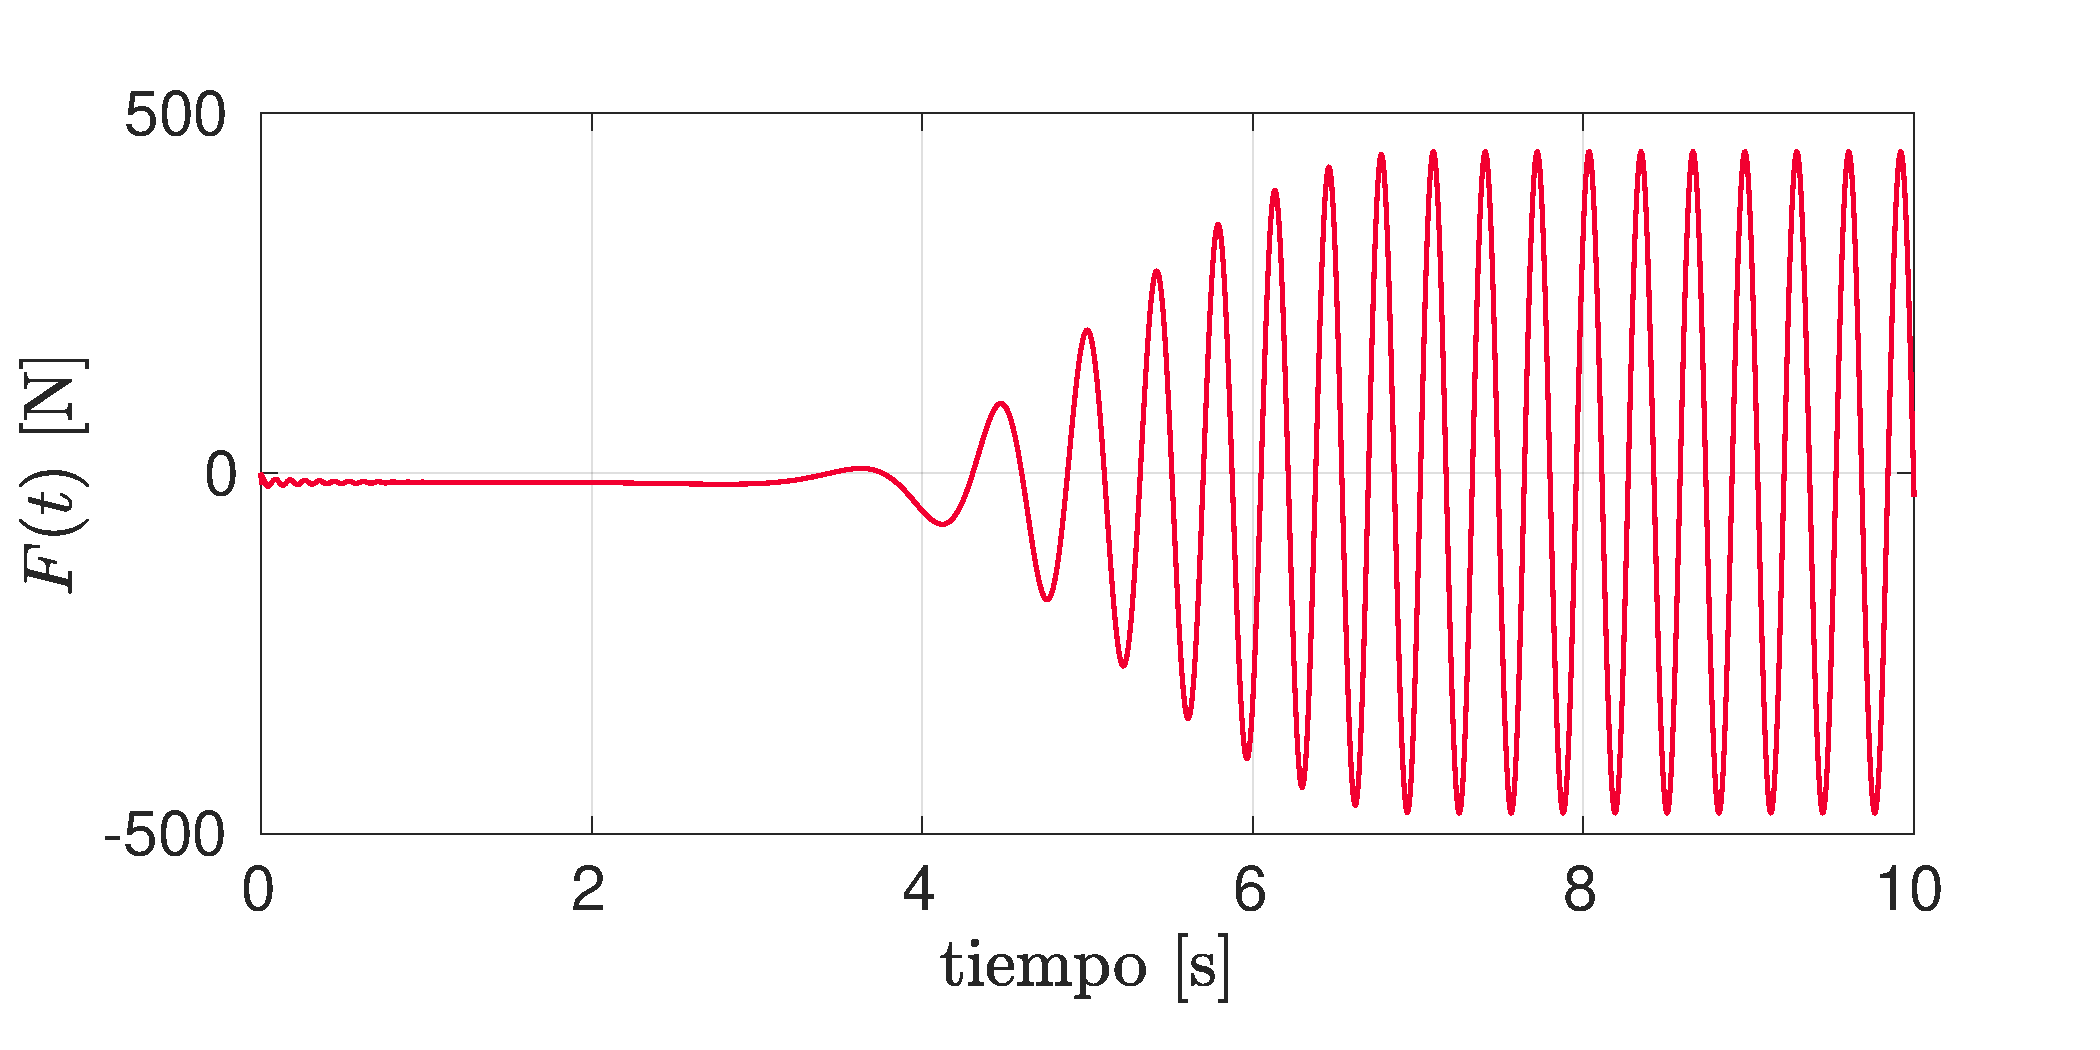
\includegraphics[width=\linewidth, trim={0cm 0cm 2cm 0cm},clip]{Imagenes/f_w20.pdf}
		\caption{Fuerza sobre la probeta a través del tiempo a $\omega_{max}=20$ [rad/s]}
		\label{fig:f_w20}
	\end{subfigure}
\caption{Comparación de la fuerza aplicada sobre la probeta $F(t)$, de la combinación (5+5+1)-(2+4), a dos velocidades angulares $\omega_{max}$ distintas.}
\label{fig:f_w520}
\end{figure}

A continuación, es posible comparar la fuerza máxima de cada combinación de contrapesos para distintas velocidades angulares $\omega_{max}$. Aquí se confirma el comportamiento descrito anteriormente para una configuración específica, pero de manera general para cada una de las 201 combinaciones existentes, como se puede ver en la imagen \ref{fig:fs_psi}. Al realizarse el conjunto de ensayos de fatiga para crear la curva $S$-$N$ a una velocidad fija, pero variando los contrapesos, se puede definir que la fuerza sobre la probeta como:
\begin{equation}\label{eq:func_psiomega}
	F(t) = f(\Psi,\: \omega_{max})
\end{equation}

Como consecuencia de los resultados que se obtuvieron del modelo, es que se hará una propuesta para corregir la tabla de carga actual, debiendo ser corroborada empíricamente a posteriori, como parte del trabajo futuro. En este sentido, es necesario conocer los esfuerzos asociados a cada combinación de contrapesos, de la misma forma que lo hace la tabla actual. Entonces, para esto se realizará una simulación de las cargas aplicadas sobre la probeta, que se obtuvieron en este análisis, en la siguiente sección. 

\begin{sidewaysfigure}[p]
\centering
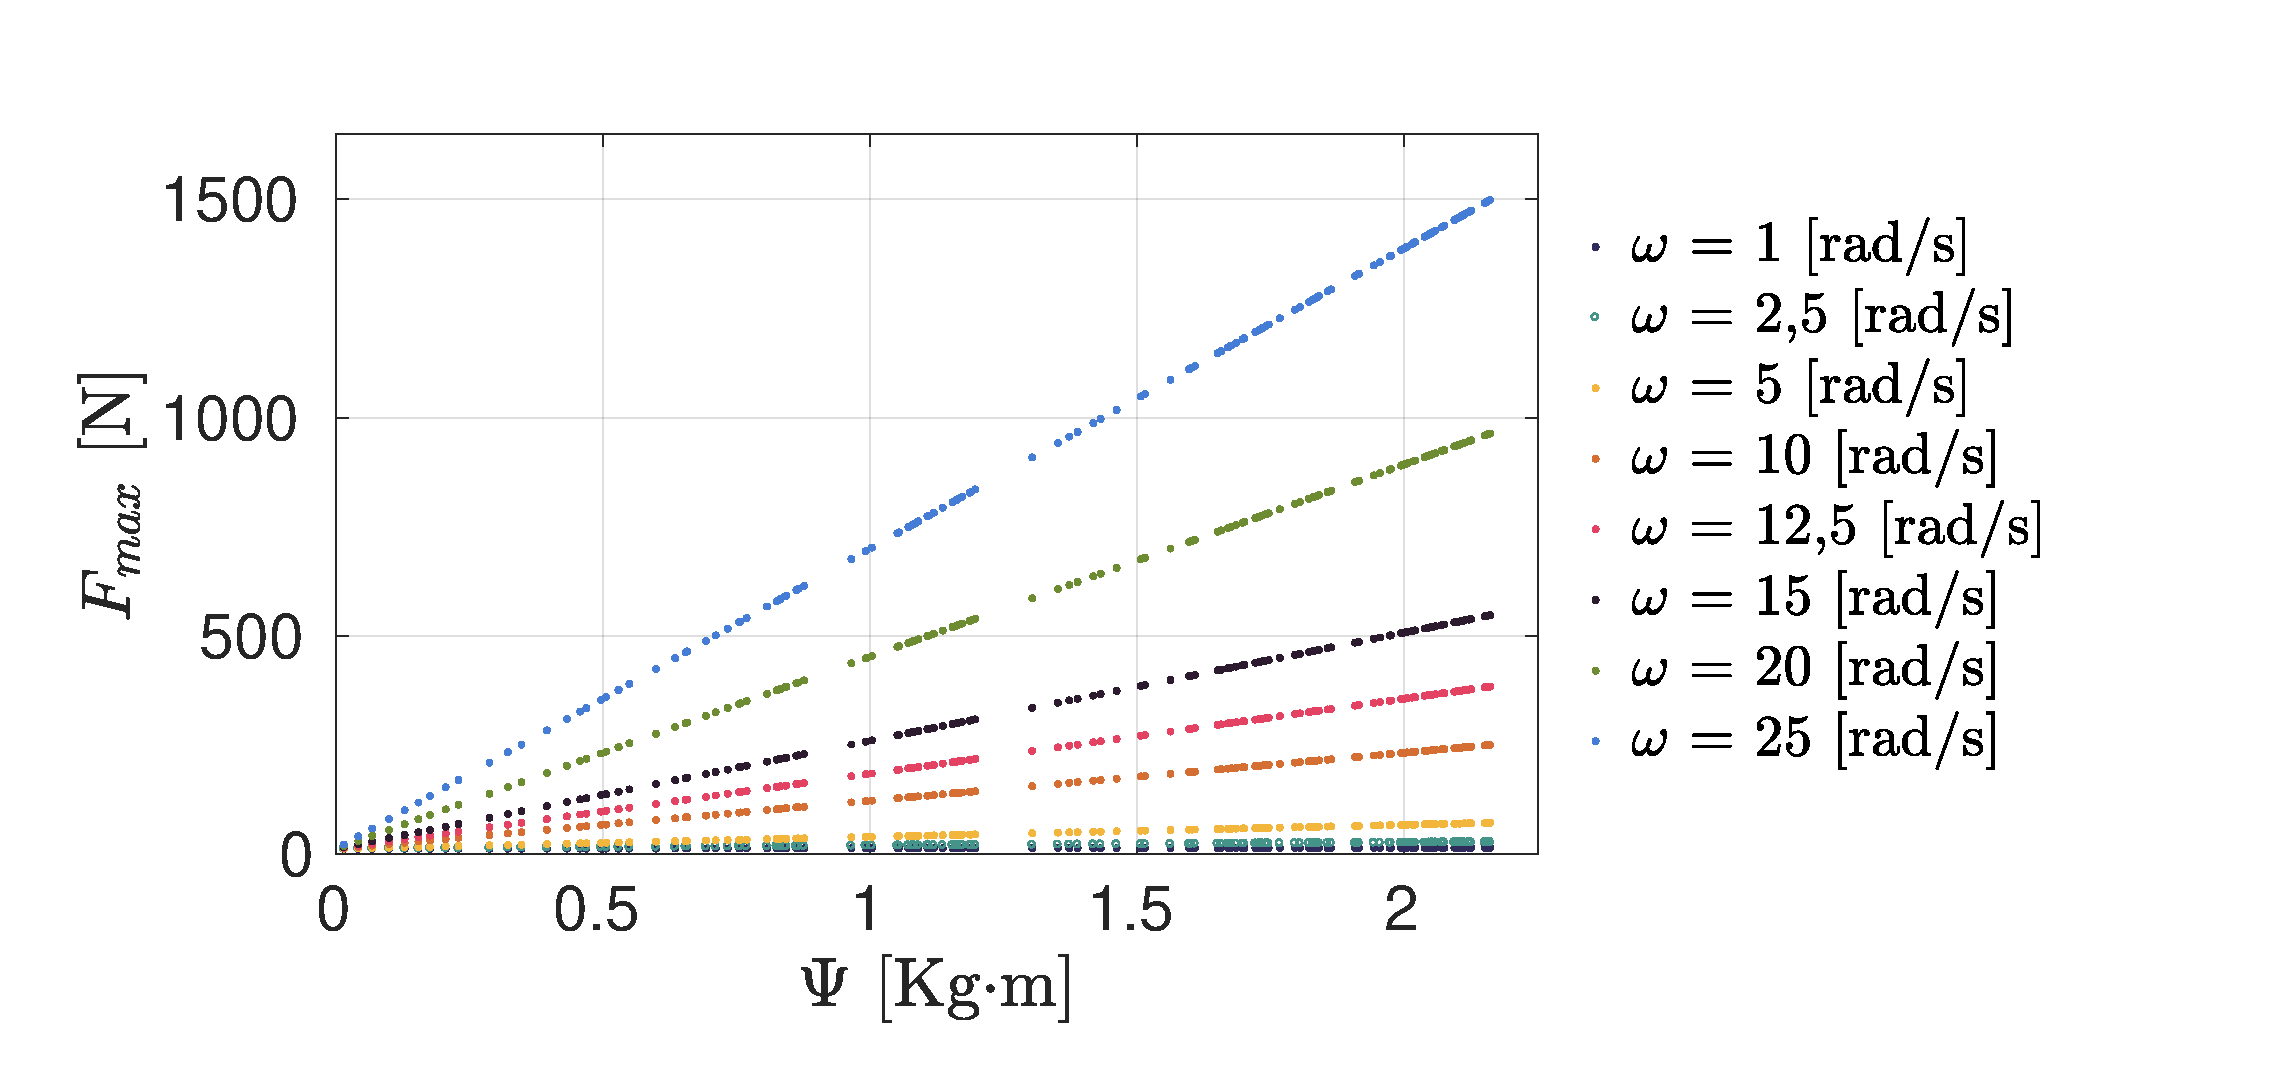
\includegraphics[width=1\linewidth, trim={1cm 1cm 4cm 1cm}, clip]{Imagenes/fs_psi2.pdf}
\caption{Curvas de cada combinación de contrapesos para distintas velocidades angulares $\omega_{max}$.}
\label{fig:fs_psi}
\end{sidewaysfigure}

\newpage

\section{Simulación de carga máxima}

Al tomar los datos de las cargas máximas obtenidas a través del modelo e ingresarlas al software de elementos finitos ANSYS, se obtienen los esfuerzos que sufre la probeta para cada carga. En primer lugar, los valores de carga se pasan a presión para ser aplicado sobre una de las caras de la probeta, utilizando la ecuación \ref{eq:p_max}. La imagen \ref{fig:f_step}, muestra las 77 cargas aplicadas a lo largo de la simulación. 

\begin{figure}[h]
\centering
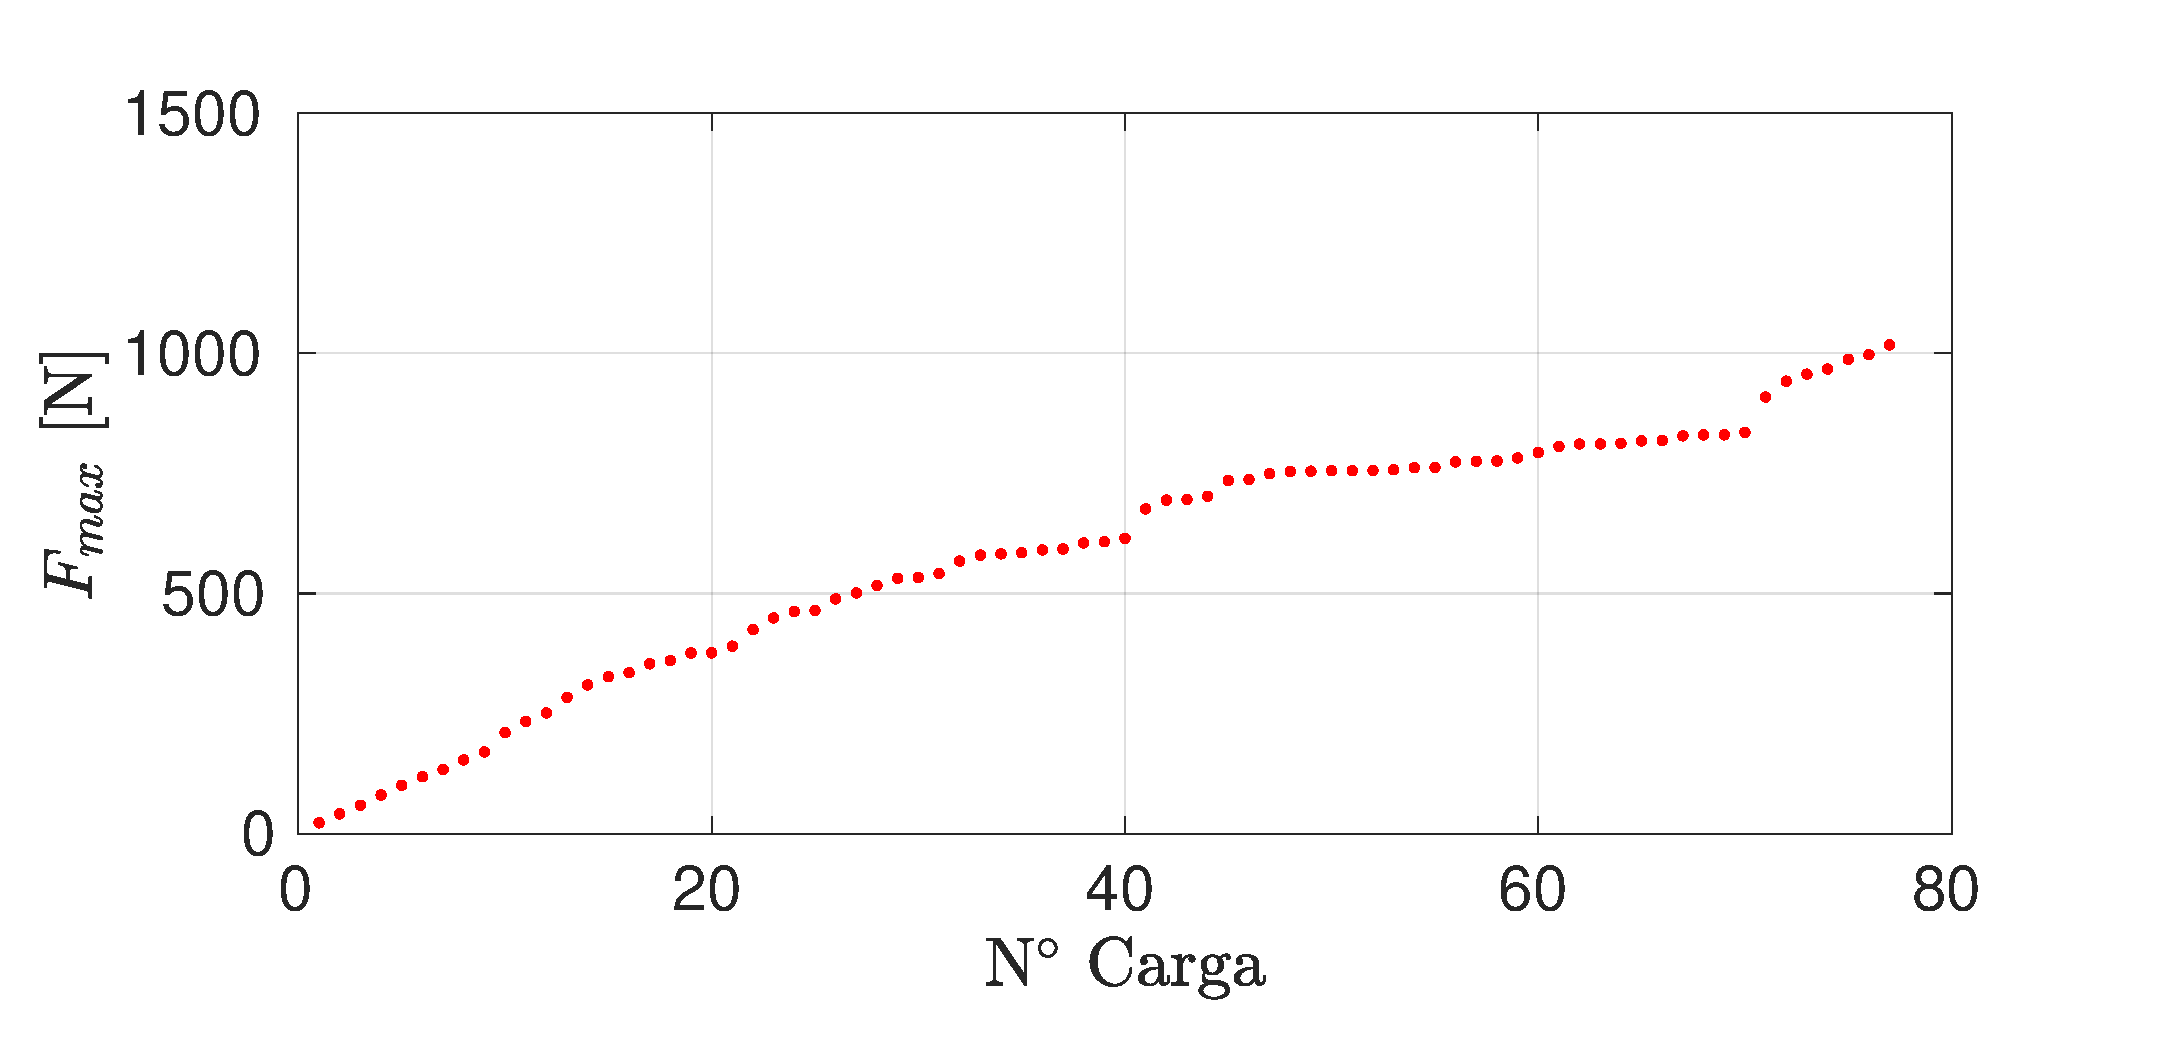
\includegraphics[width=1\linewidth, trim={2cm 5.2cm 1cm 5.2cm}, clip]{Imagenes/f_step.pdf}
\caption{Curva de las 77 cargas aplicadas sobre la probeta.}
\label{fig:f_step}
\end{figure}

Al ver los esfuerzos generales a los que está sometida la probeta, se identifica que la zona más afectada es la intermedia, concentrándose justo en la mitad de la probeta, como se ve en las imágenes \ref{fig:r_lat} y \ref{fig:r_iso}. Al realizar un corte transversal en la mitad de la probeta (imagen \ref{fig:rcorte_iso}) se pueden apreciar más claramente la distribución de los esfuerzos equivalentes en la zona intermedia, concentrandose fuertemente en la zona inferior y superior de la cara transversal. La imagen \ref{fig:rcorte} muestra directamente la cara sometida a la carga máxima y su distribución de esfuerzos, donde además, se puede ver que la zona cercana al eje neutro tiene esfuerzos menores a los que se encuentran más lejos de este. Esta información es posible verla directamente en el comportamiento que tienen los elementos  $P$, $Q$ y $R$.

\begin{figure}[p]
\centering
	\begin{subfigure}{0.8\linewidth}
		\centering
		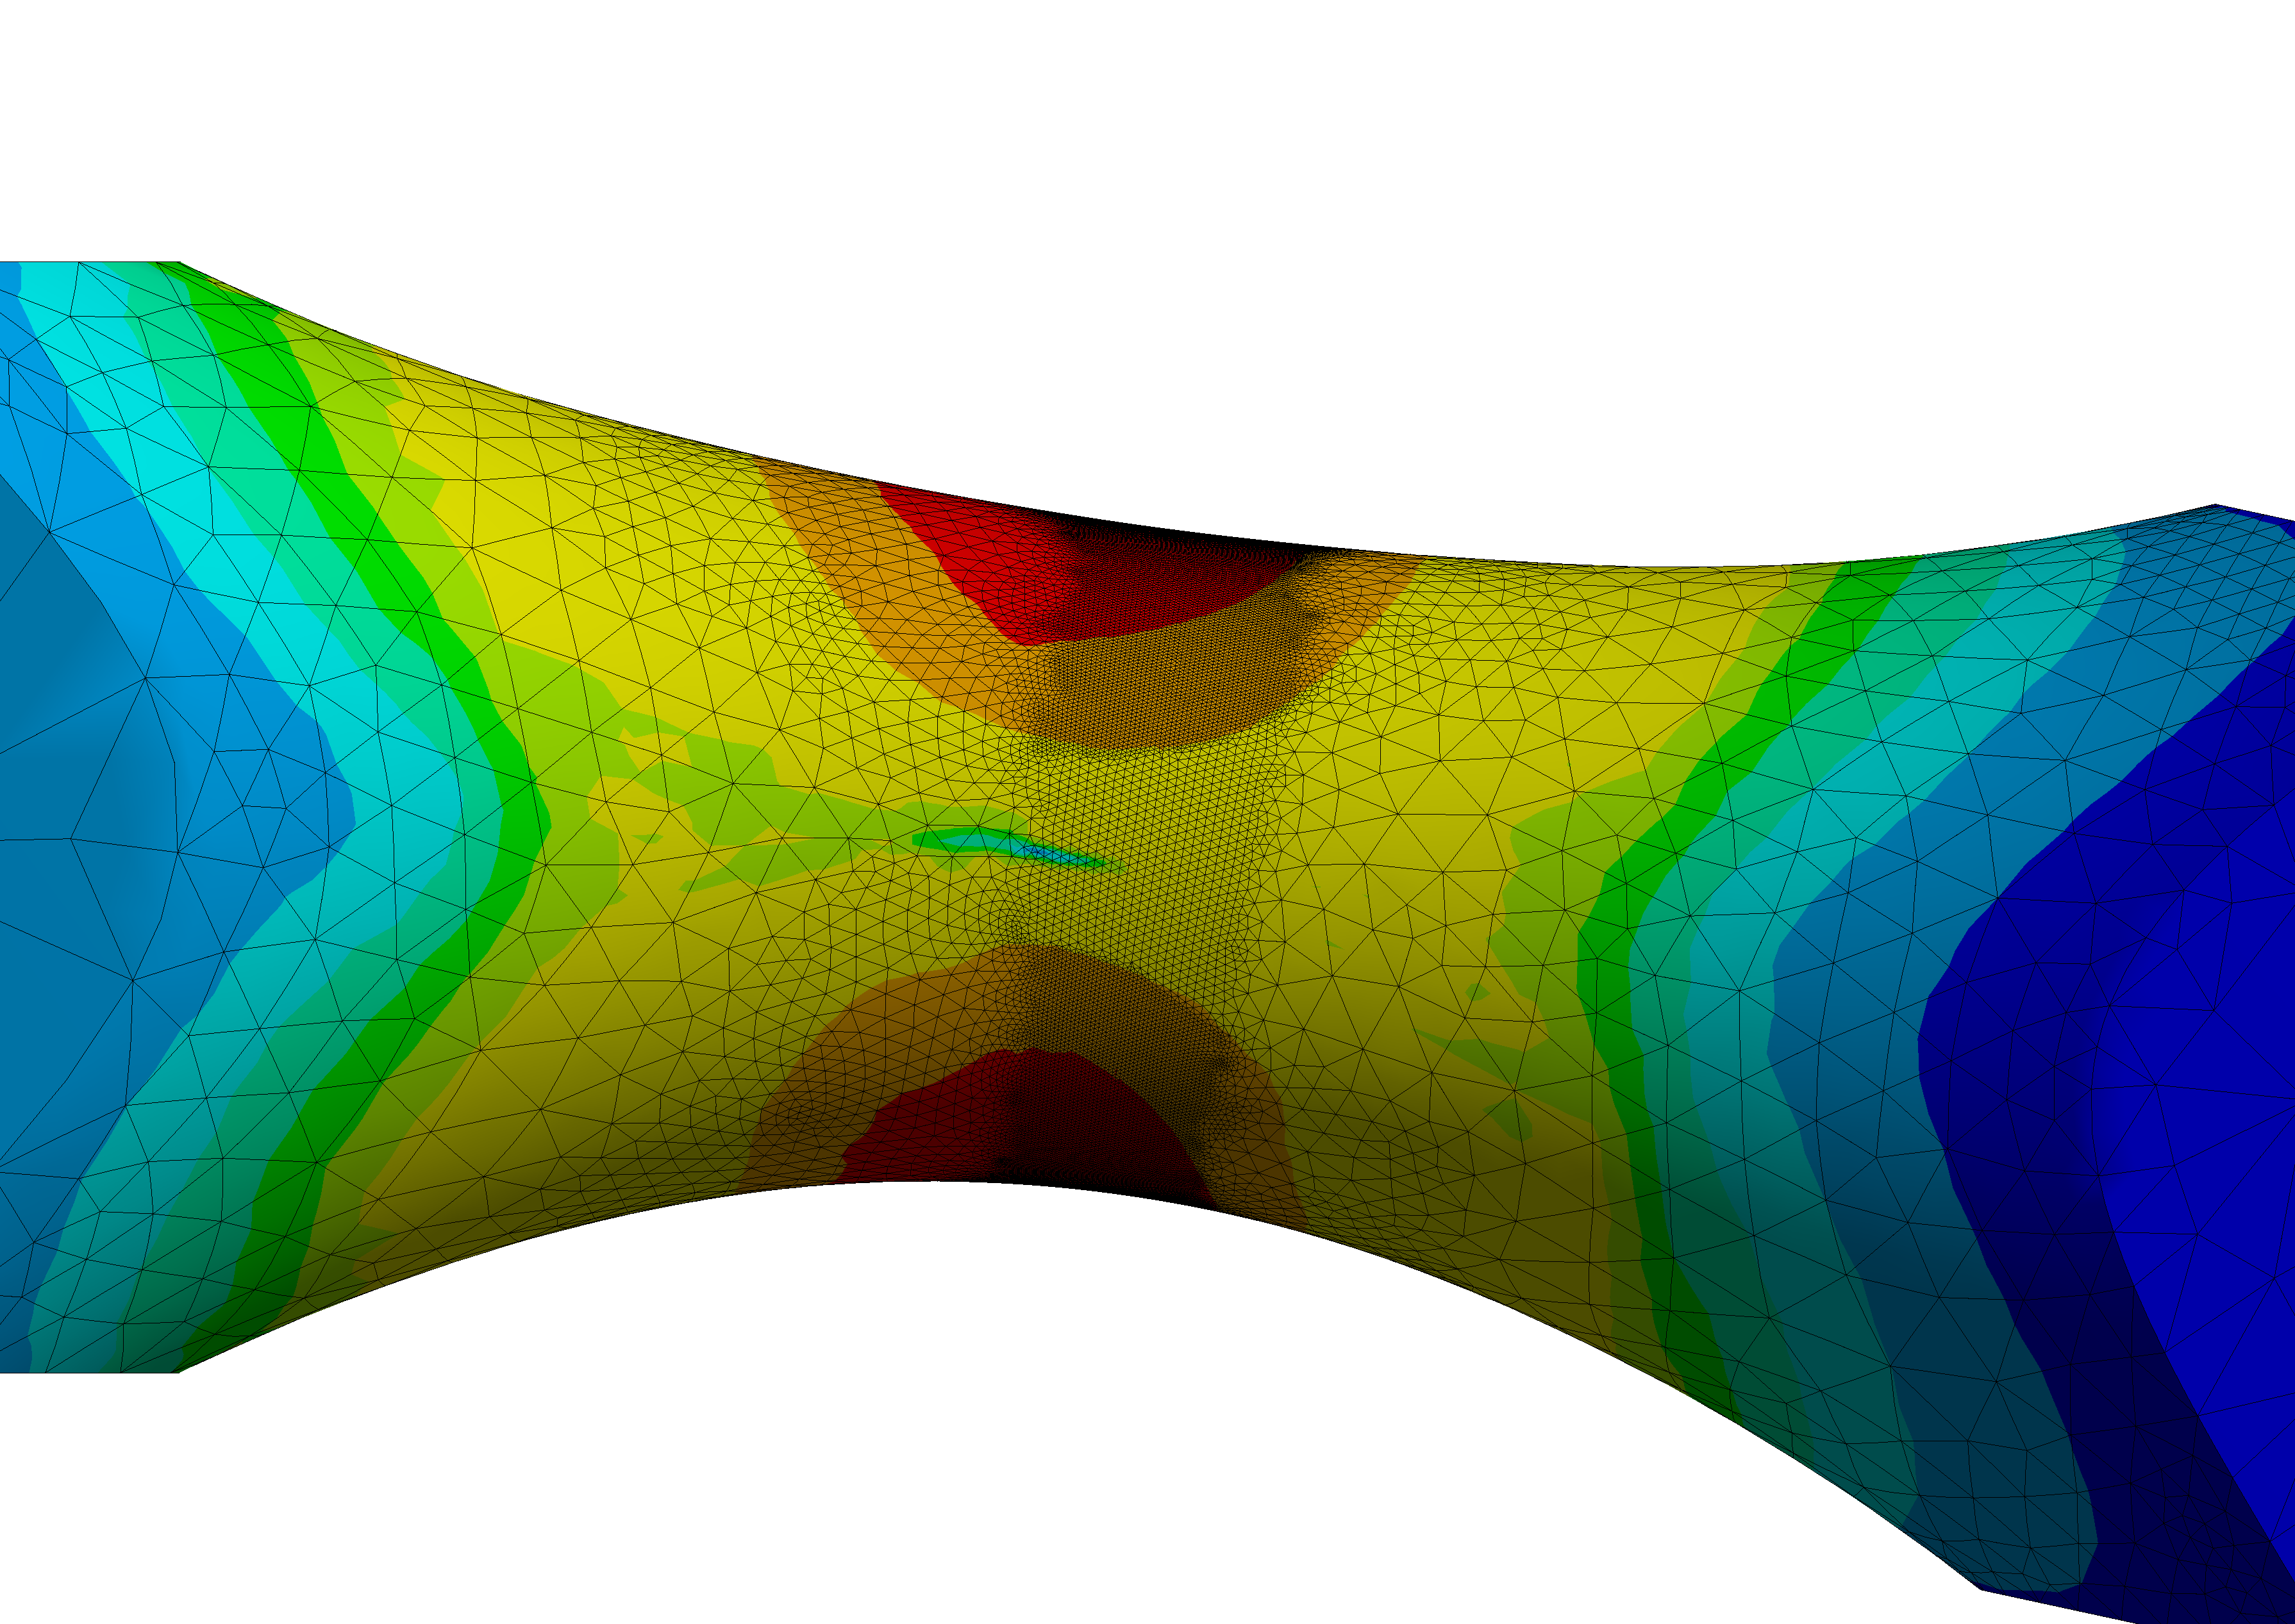
\includegraphics[width=\linewidth]{Imagenes/r_lat.png}
		\caption{Vista lateral de la zona intermedia.}
		\label{fig:r_lat}
	\end{subfigure}
	\begin{subfigure}{0.8\linewidth}
		\centering
		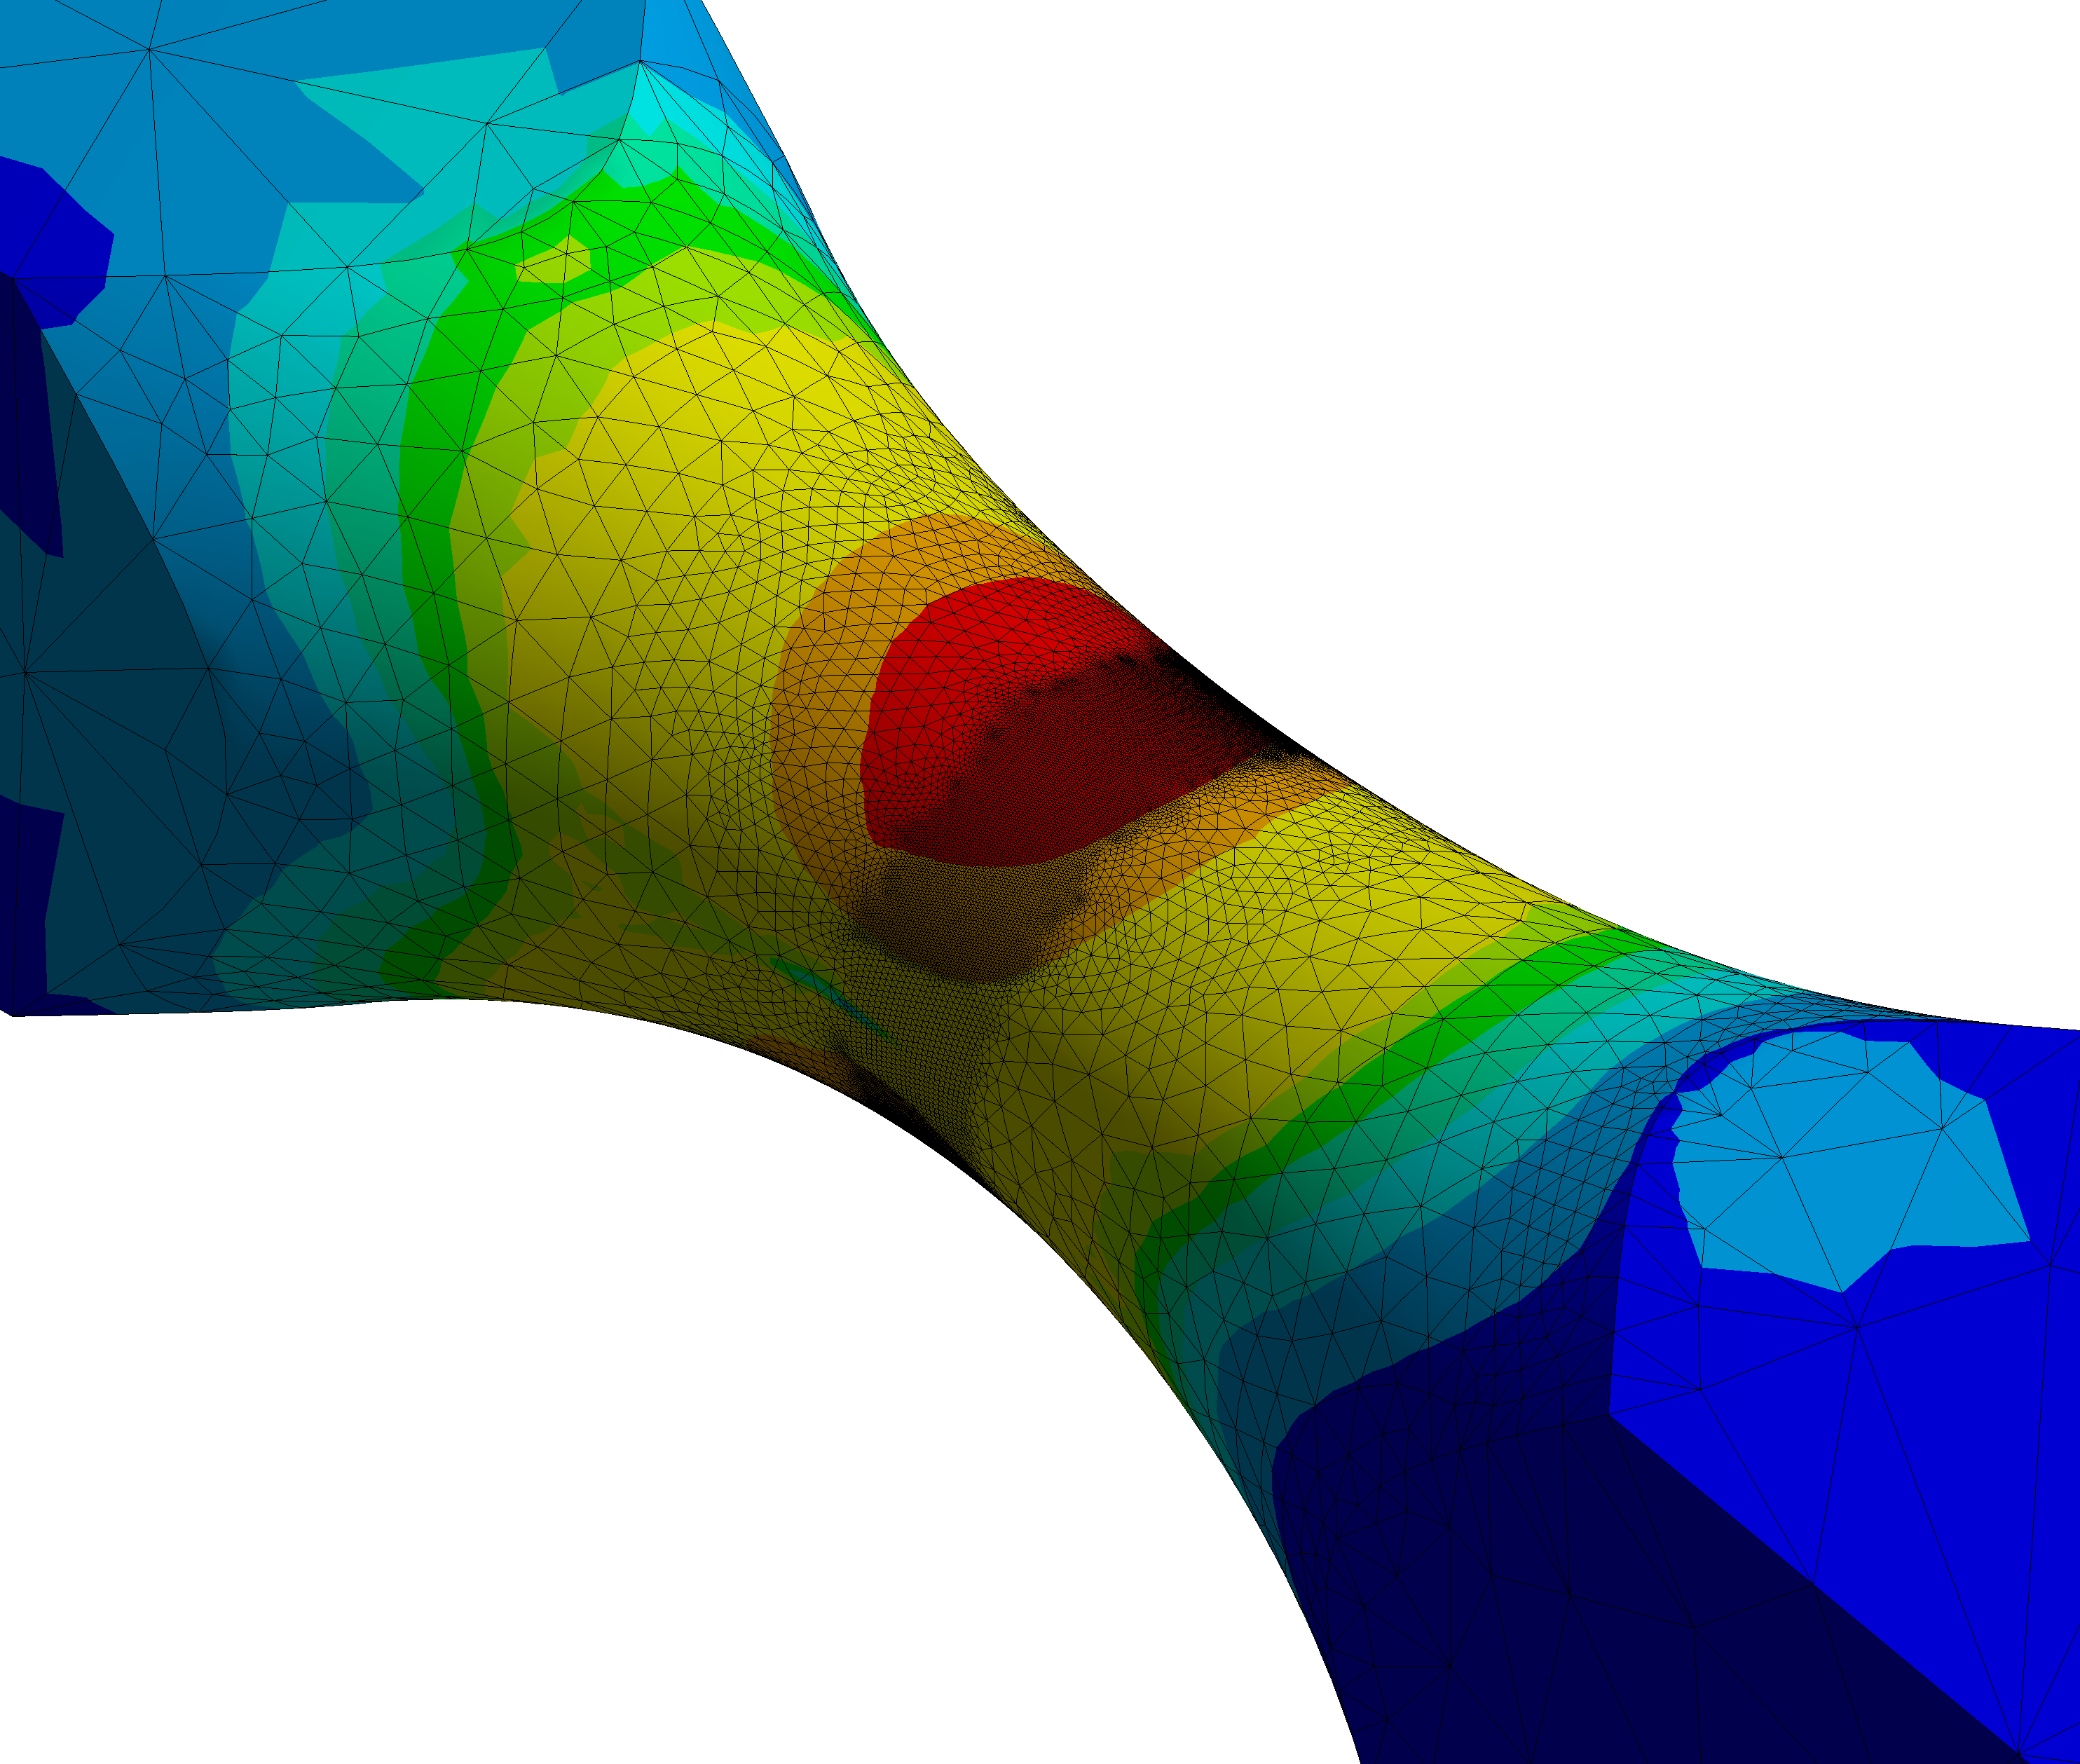
\includegraphics[width=\linewidth]{Imagenes/r_iso.png}
		\caption{Vista en isométrico de la zona intermedia.}
		\label{fig:r_iso}
	\end{subfigure}
\end{figure}
\begin{figure}[]
	\ContinuedFloat
	\centering
	\begin{subfigure}{0.6\linewidth}
		\centering
		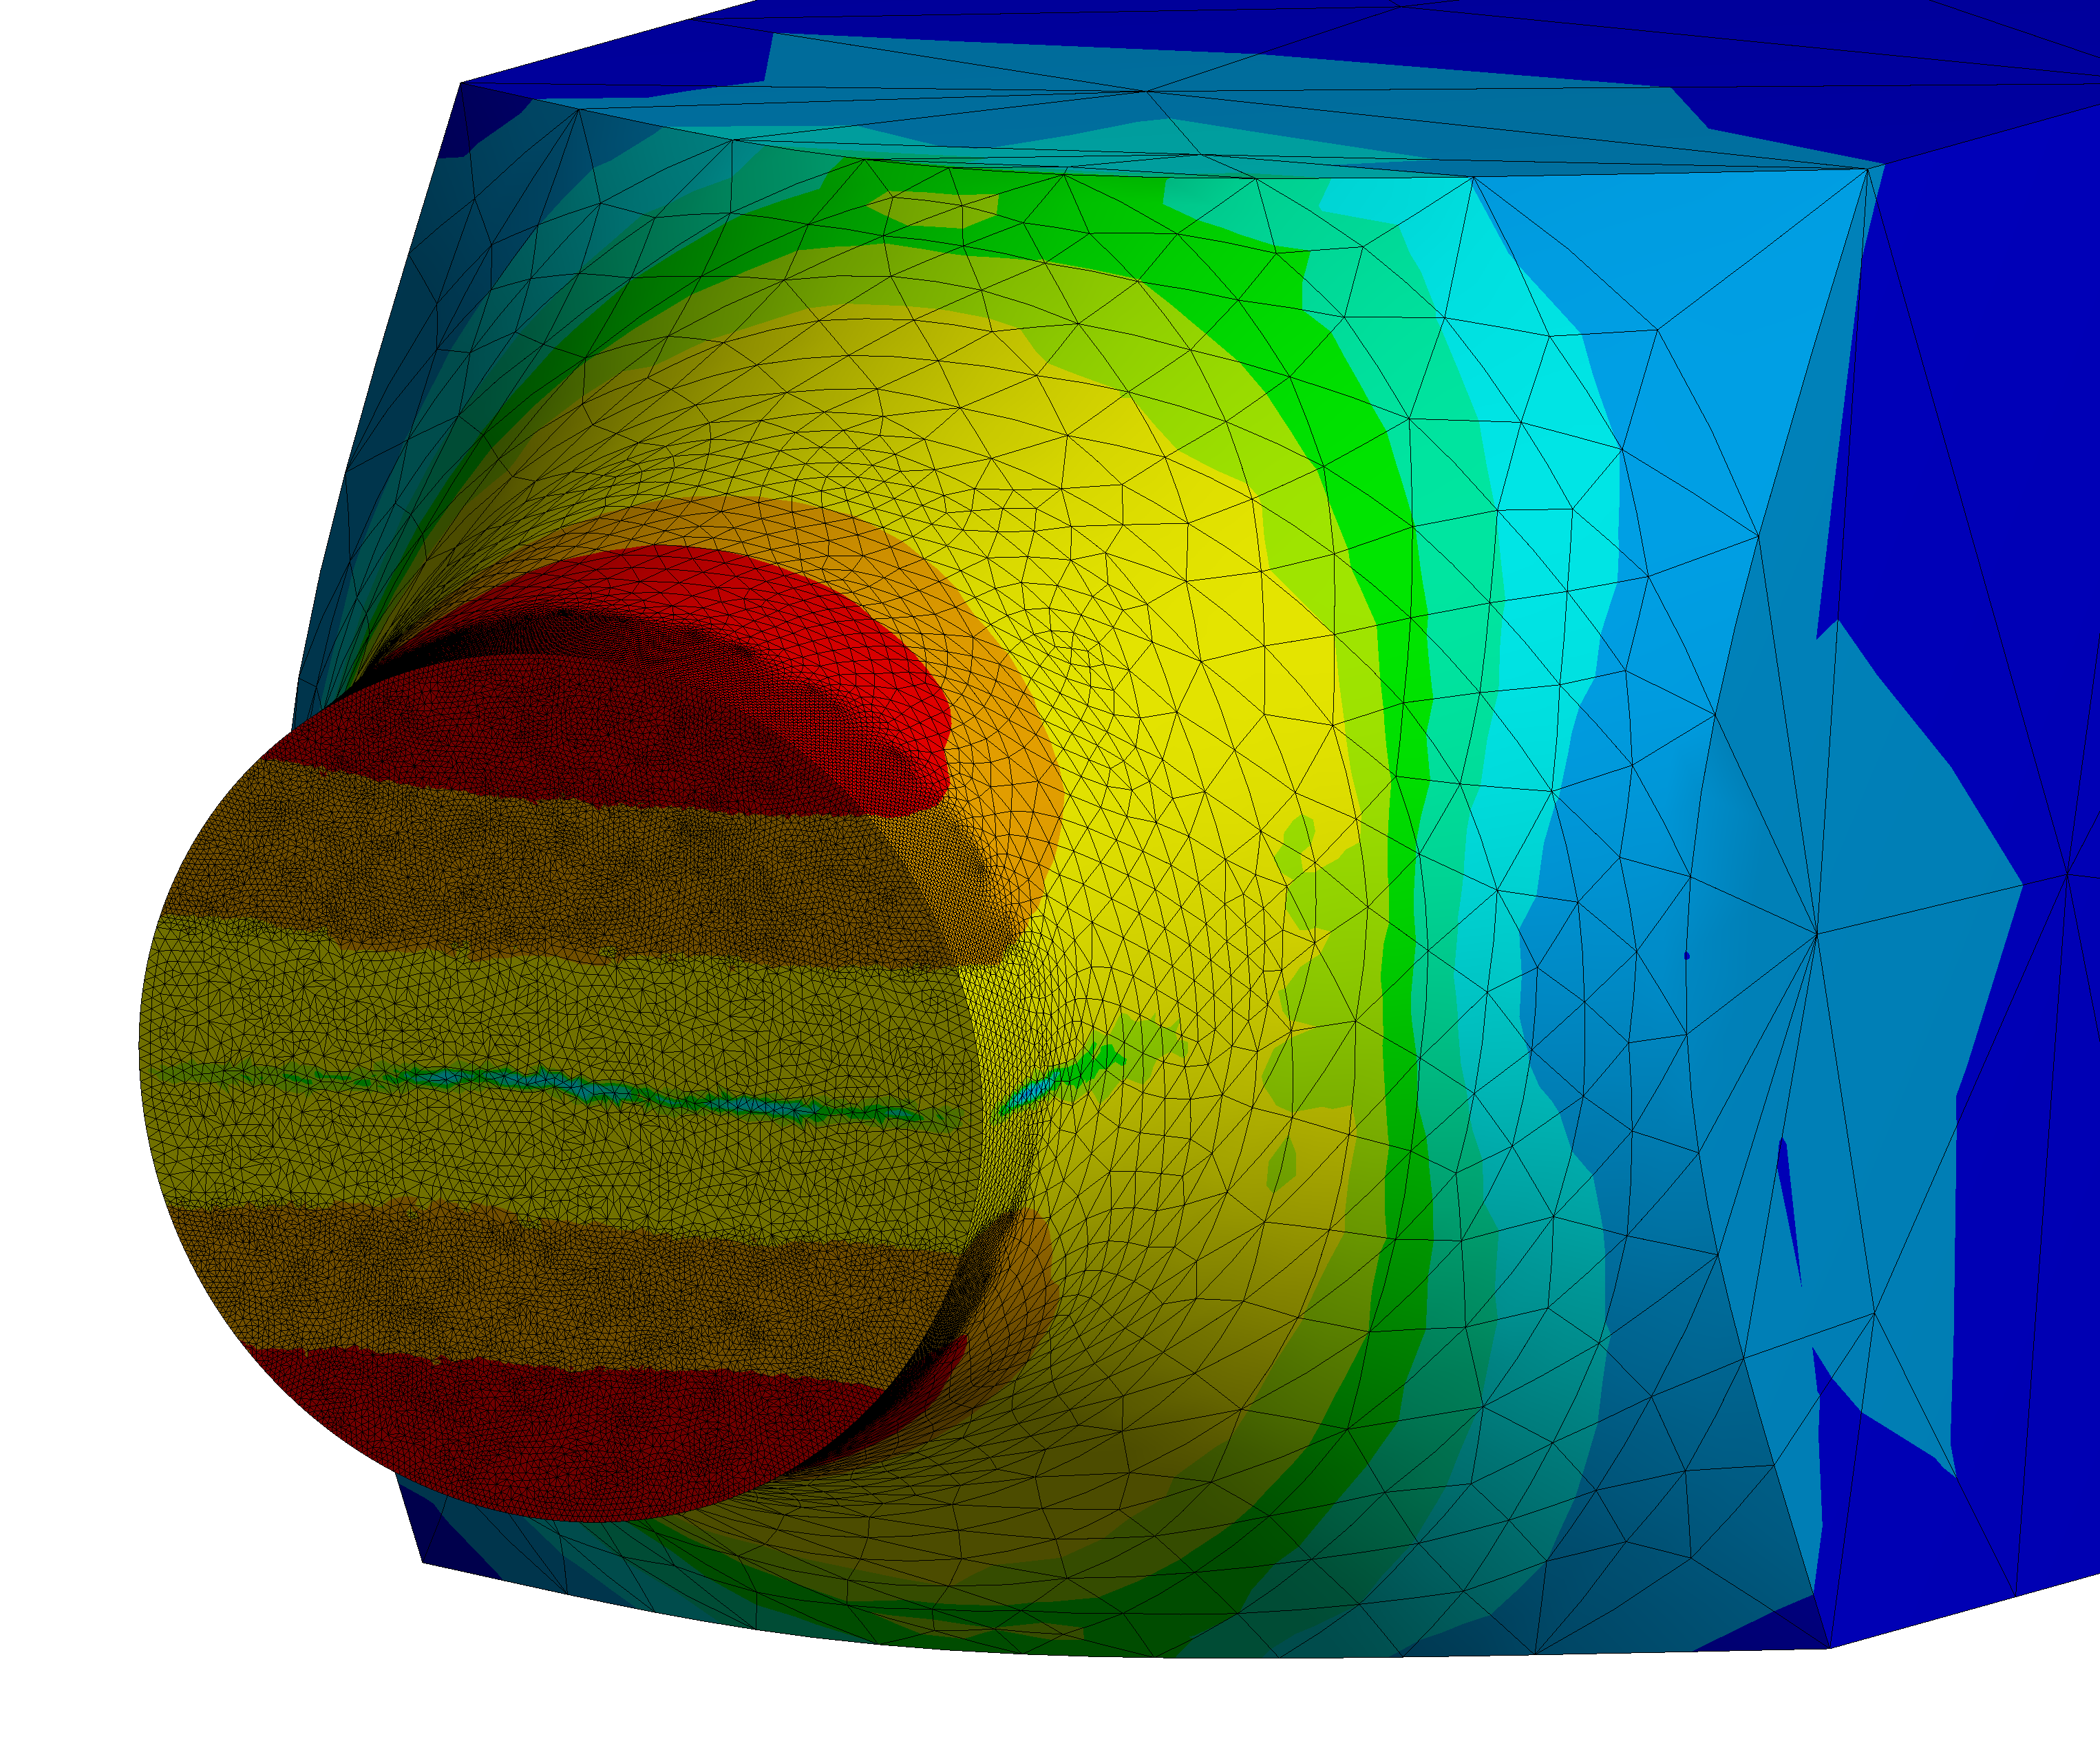
\includegraphics[width=\linewidth]{Imagenes/rcorte_iso.png}
		\caption{Vista en isométrico del corte transversal.}
		\label{fig:rcorte_iso}
	\end{subfigure}		
	\begin{subfigure}{0.6\linewidth}
		\centering
		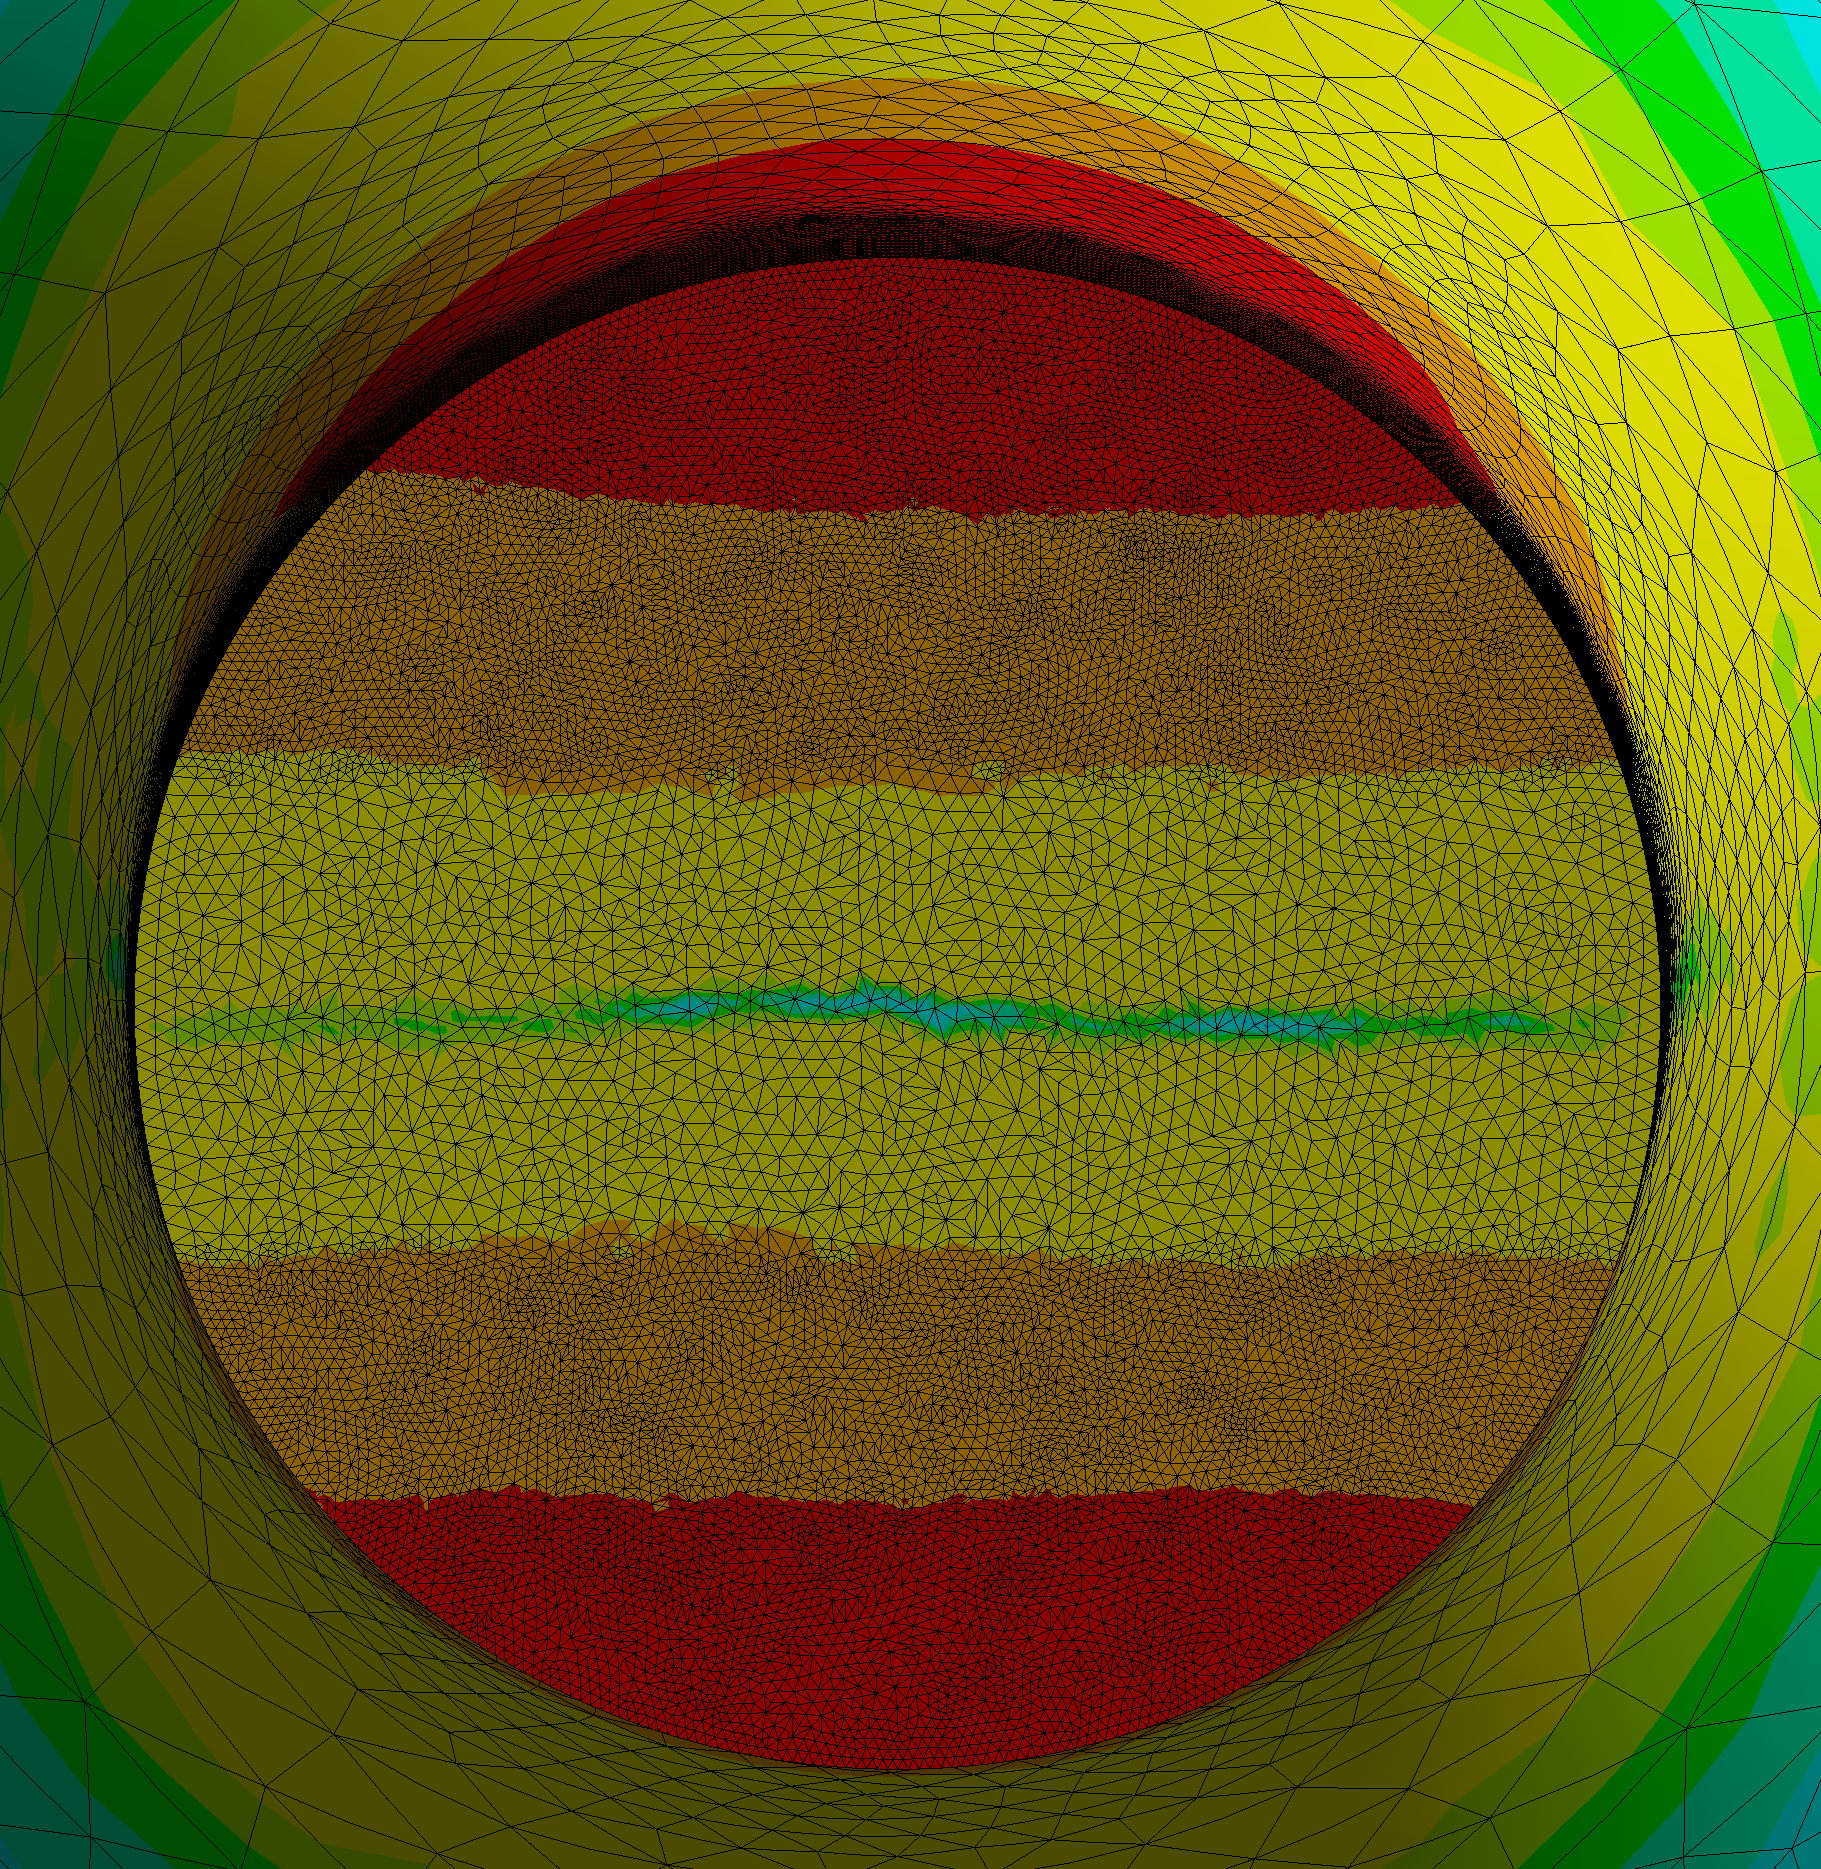
\includegraphics[width=\linewidth]{Imagenes/rcorte.png}
		\caption{Vista en detalle del corte transversal.}
		\label{fig:rcorte}
	\end{subfigure}
\caption{Detalle de la distribución de esfuerzos equivalentes en la zona intermedia de la probeta.}
\label{fig:resultados_vm}
\end{figure}

\newpage

Por último, como se buscan conocer los esfuerzos a los que está sometida la probeta en estos puntos en específico, se obtienen los resultados de la deformación unitaria normal ($\varepsilon_x$) y equivalente total ($\varepsilon_{vm,t}$), además de los esfuerzos de von Mises ($\sigma_{vm}$), normal ($\sigma_x$) y cortante máximo ($\tau_{max}$). Estos resultados se pueden ver en los gráficos \ref{fig:def_pqr} y \ref{fig:esf_pqr}.

\begin{figure}[h]
\centering
	\begin{subfigure}{1\linewidth}
		\centering
		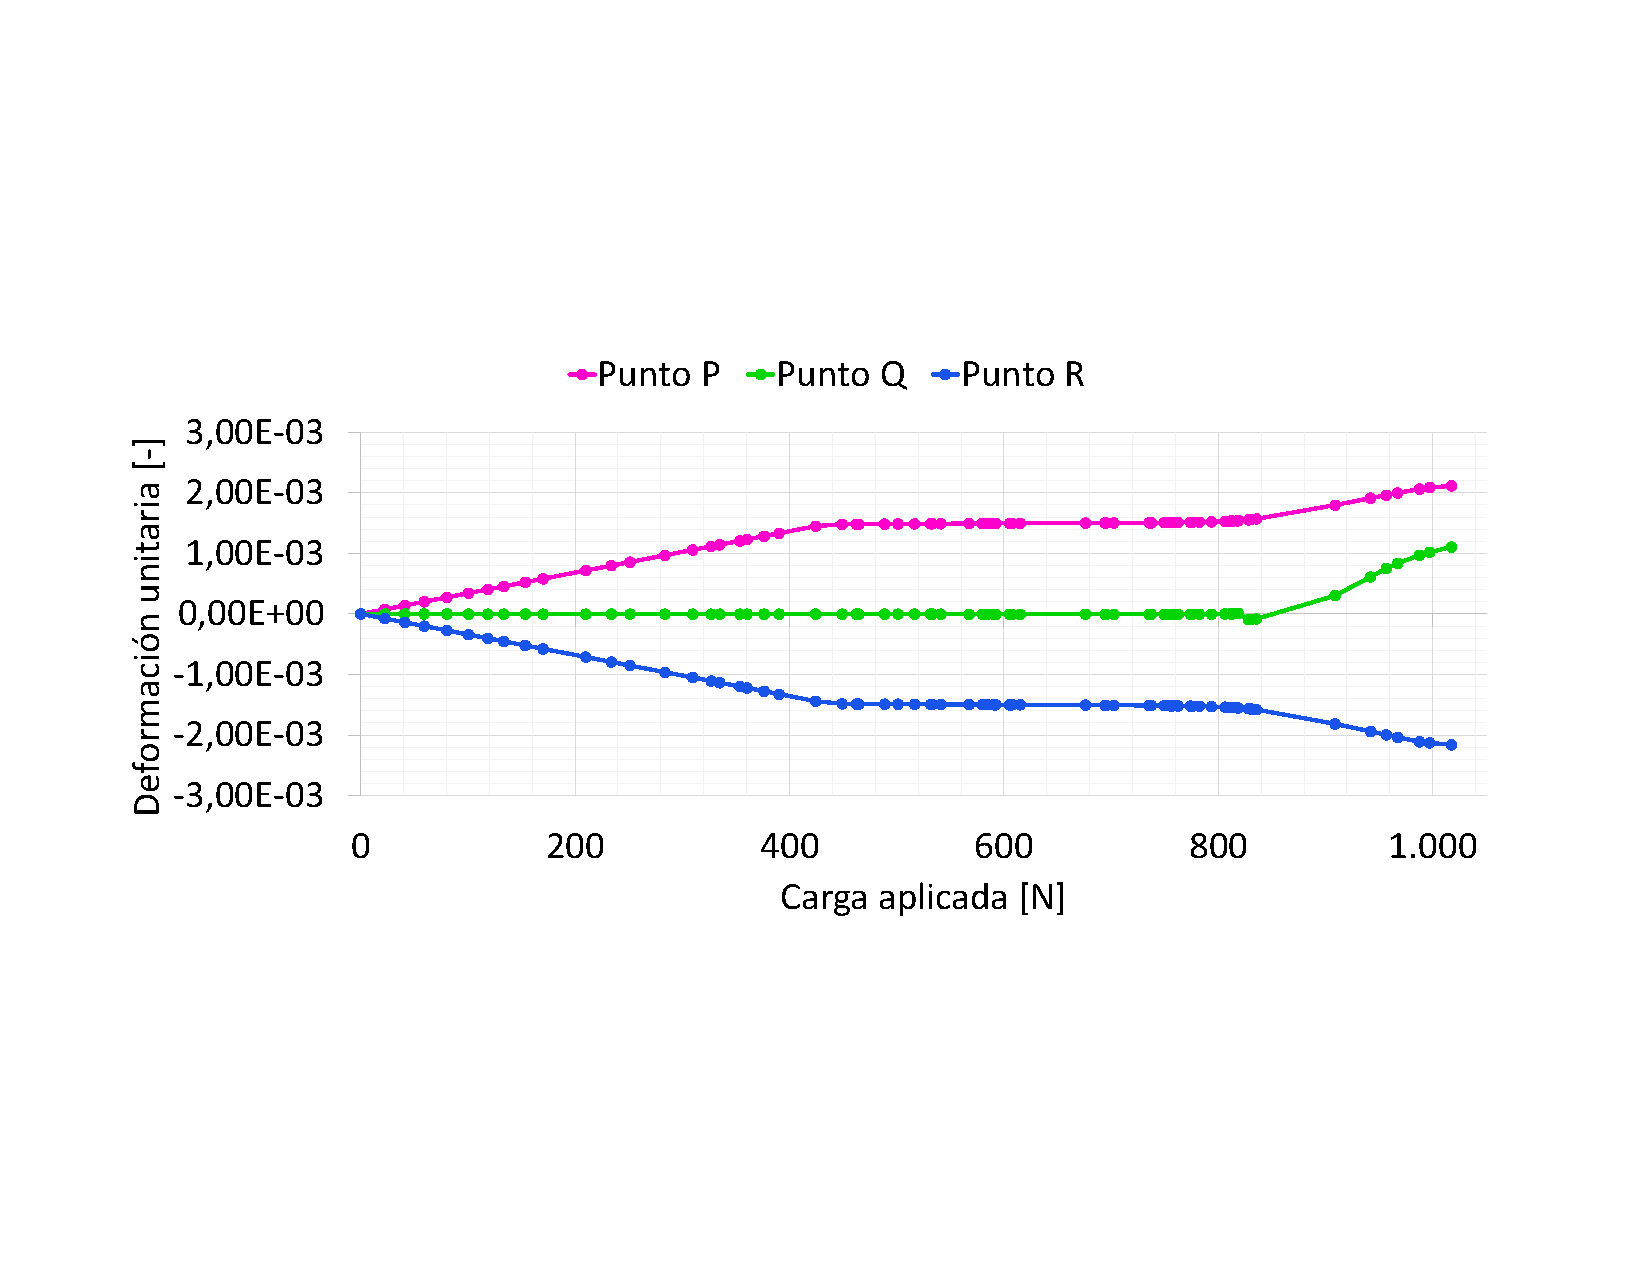
\includegraphics[width=\linewidth, trim={2cm 5cm 2cm 5cm},clip]{Imagenes/defpqr_normal.pdf}
		\caption{Deformación normal, en dirección $x$, de los puntos $P$, $Q$ y $R$.}
		\label{fig:defpqr_normal}
	\end{subfigure}
		\begin{subfigure}{1\linewidth}
		\centering
		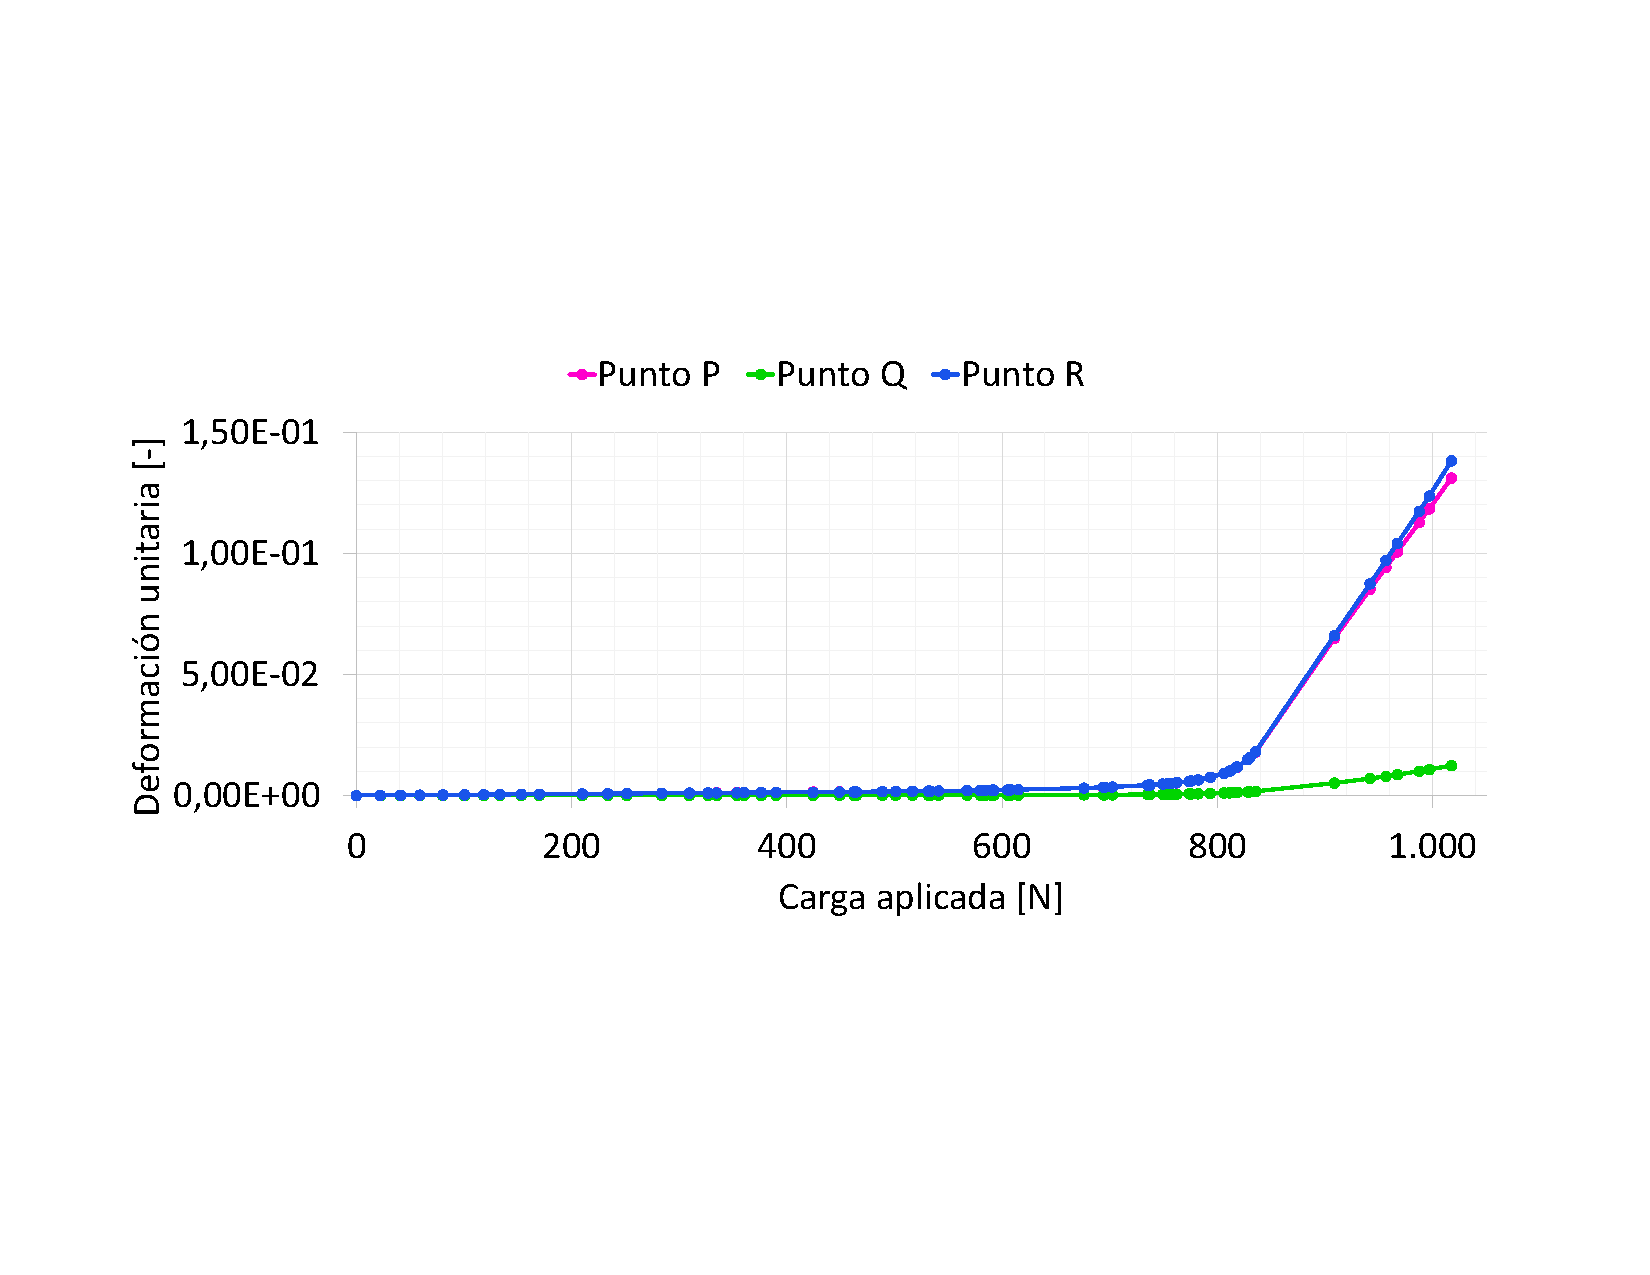
\includegraphics[width=\linewidth, trim={2cm 5cm 2cm 5cm},clip]{Imagenes/defpqr_vmt.pdf}
		\caption{Deformación equivalente total de los puntos $P$, $Q$ y $R$.}
		\label{fig:defpqr_vmt}
	\end{subfigure}
\caption{Deformación unitaria de los puntos $P$, $Q$ y $R$  }
\label{fig:def_pqr}
\end{figure}

\newpage

\begin{figure}[H]
\centering
	\begin{subfigure}{1\linewidth}
		\centering
		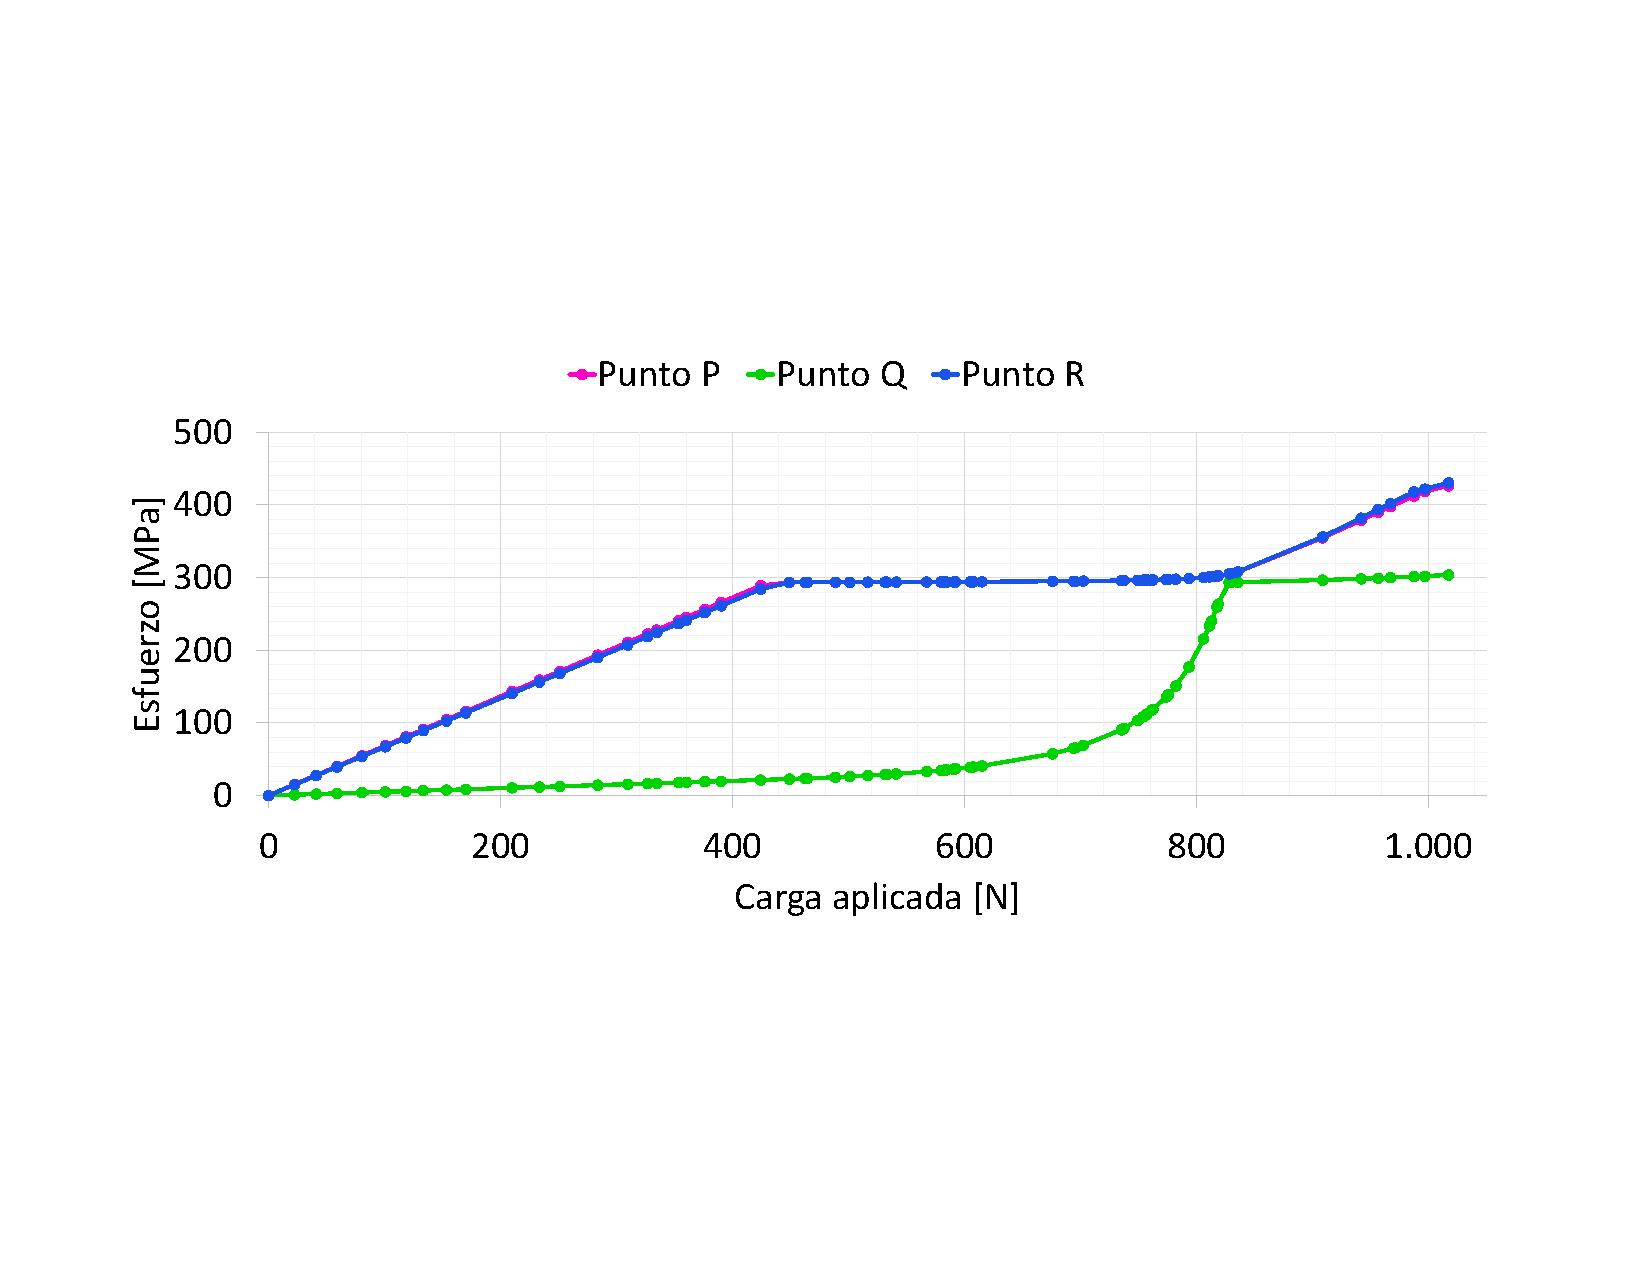
\includegraphics[width=\linewidth, trim={2cm 5cm 2cm 5cm},clip]{Imagenes/esfpqr_vm.pdf}
		\caption{Esfuerzo de von Mises de los puntos $P$, $Q$ y $R$.}
		\label{fig:esfpqr_vm}
	\end{subfigure}
	\begin{subfigure}{1\linewidth}
		\centering
		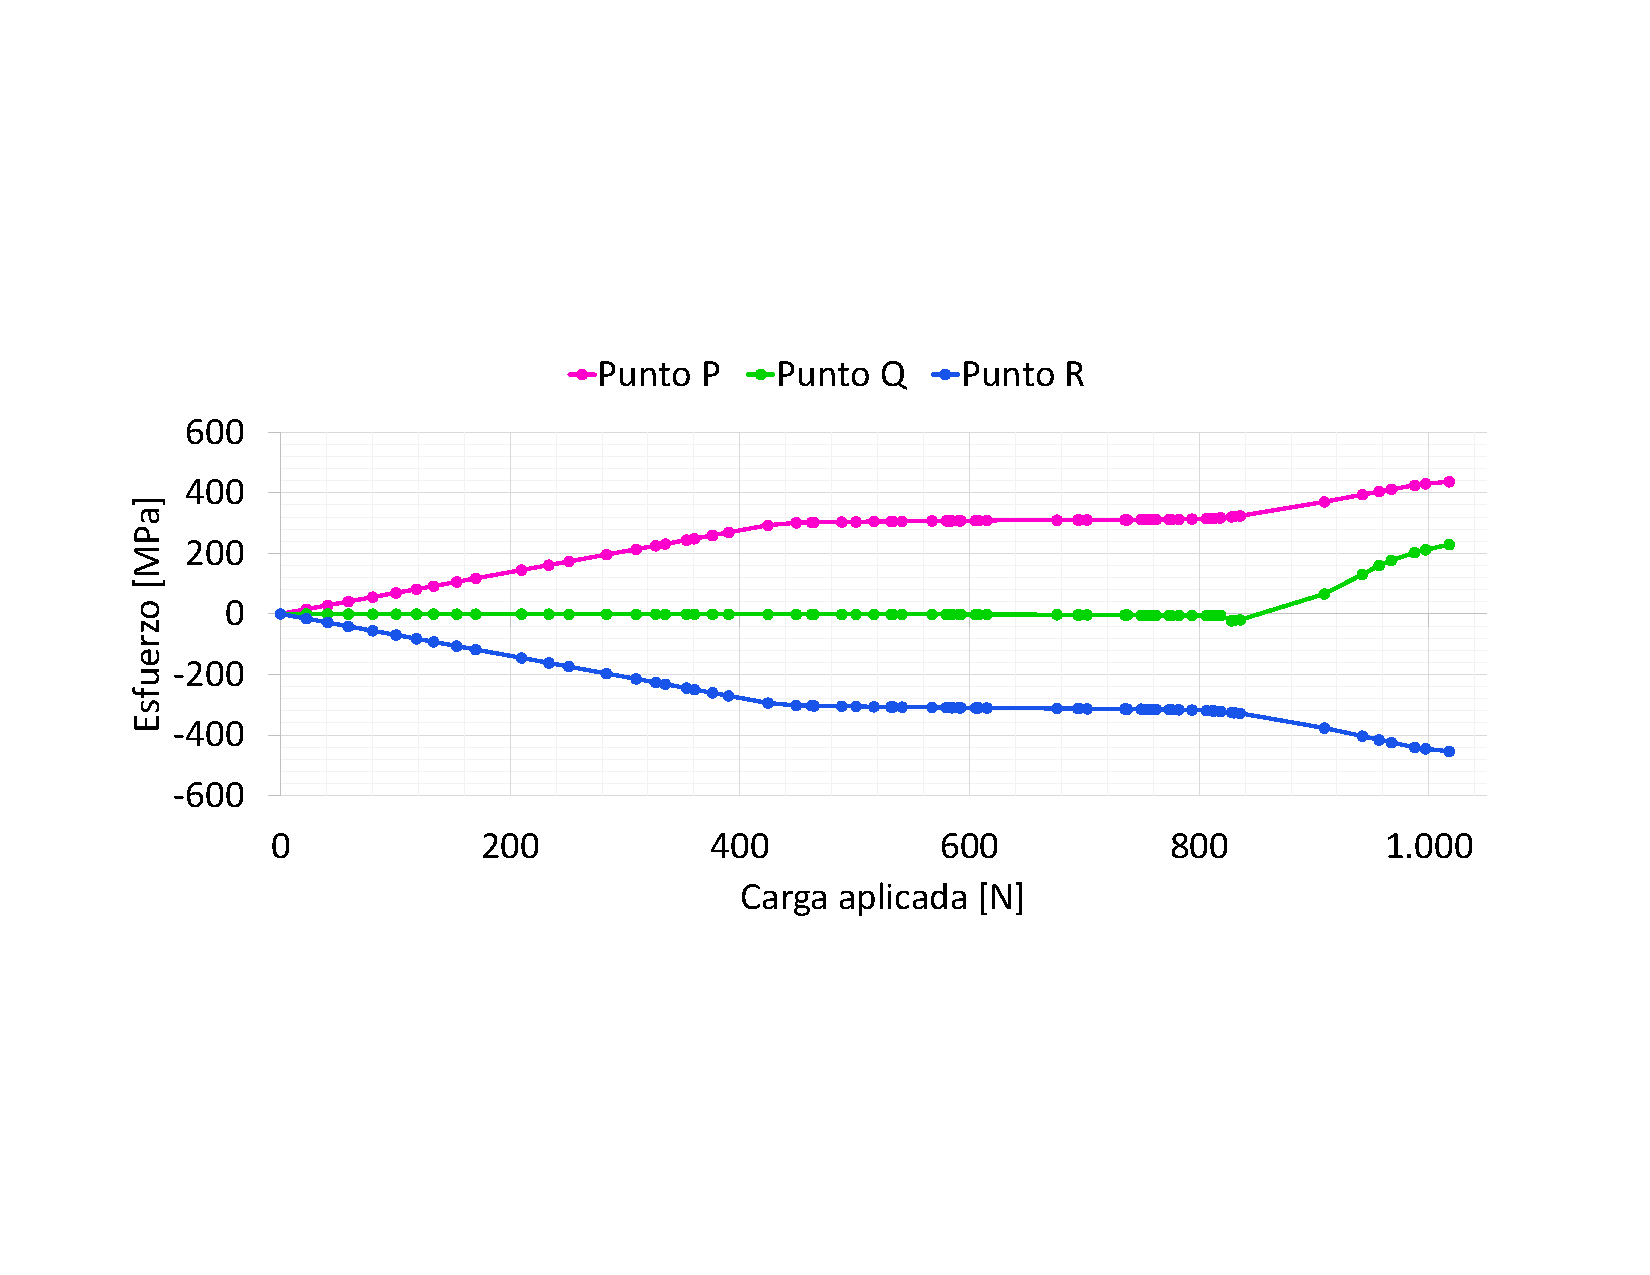
\includegraphics[width=\linewidth, trim={2cm 5cm 2cm 5cm},clip]{Imagenes/esfpqr_normal.pdf}
		\caption{Esfuerzo normal, en dirección $x$, de los puntos $P$, $Q$ y $R$.}
		\label{fig:defpqr_vmt}
	\end{subfigure}
	\begin{subfigure}{1\linewidth}
		\centering
		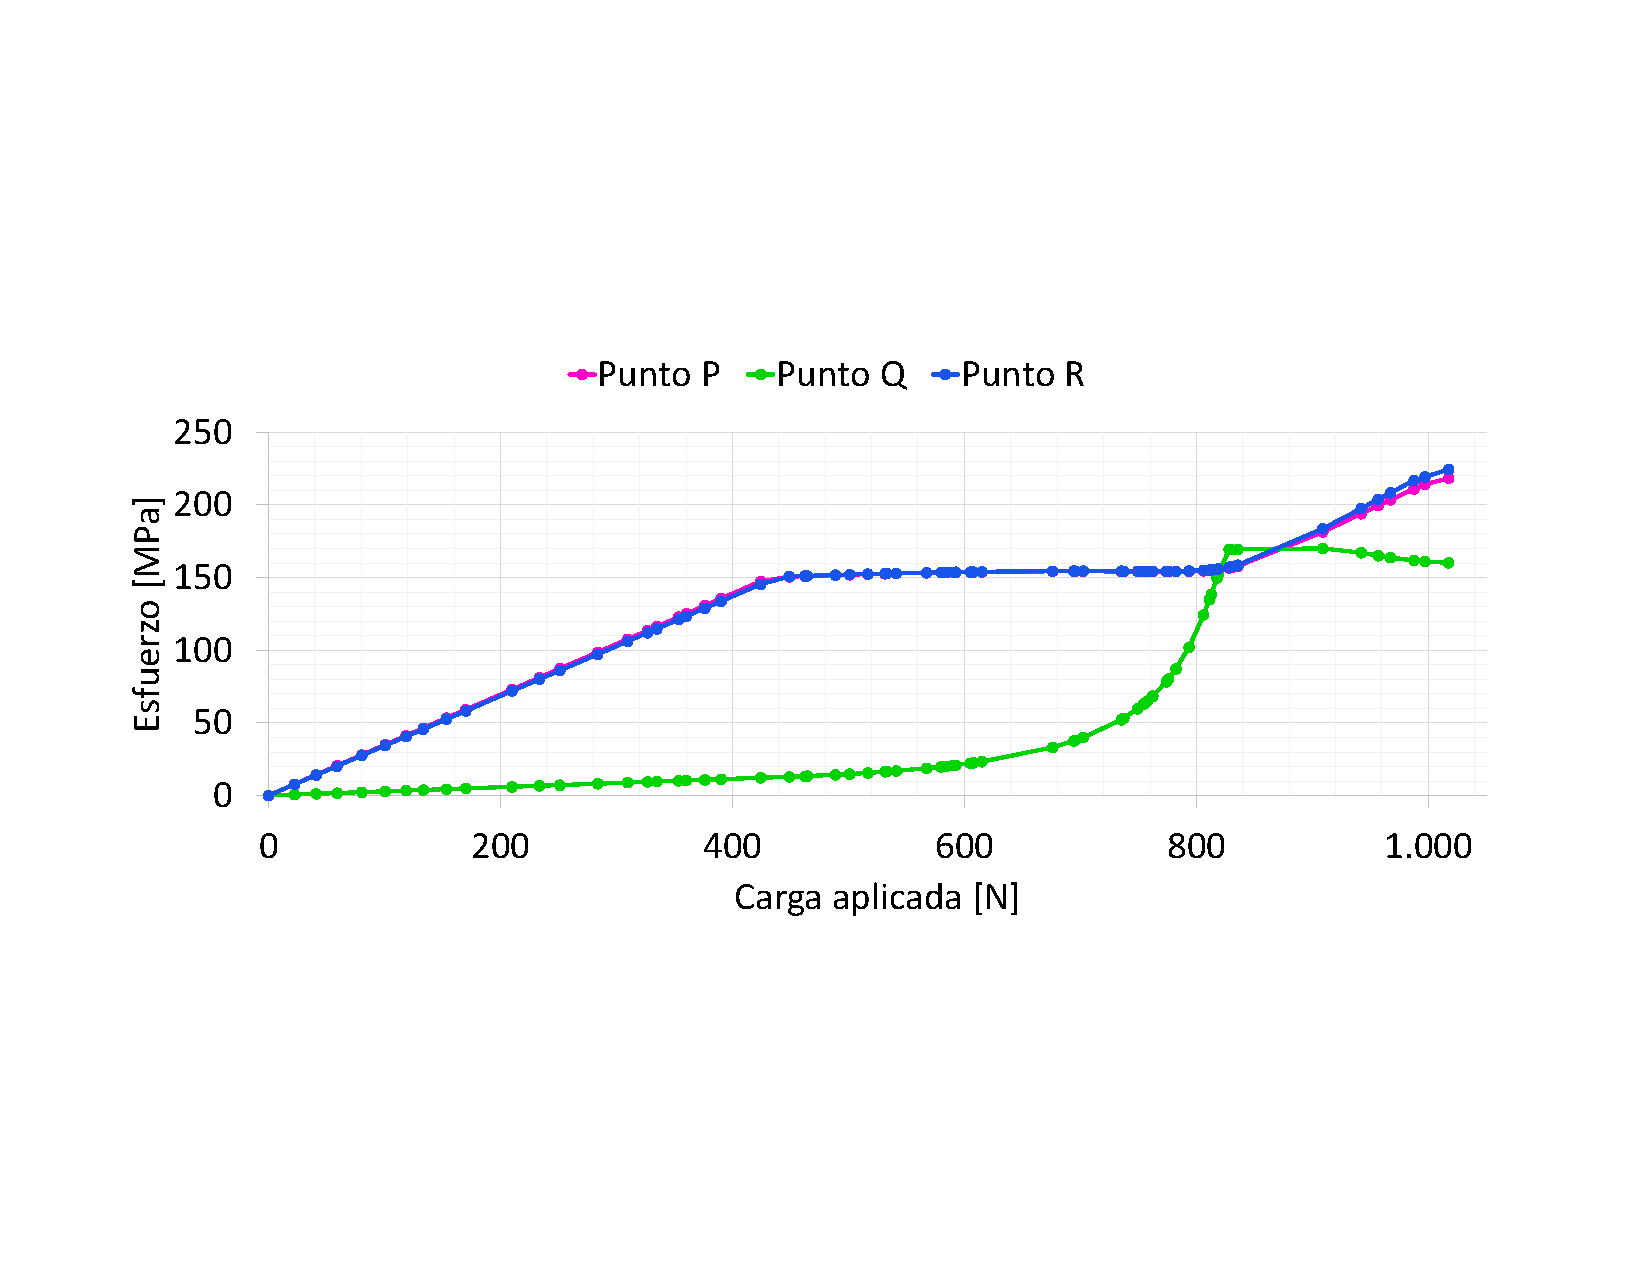
\includegraphics[width=\linewidth, trim={2cm 5cm 2cm 5cm},clip]{Imagenes/esfpqr_ms.pdf}
		\caption{Esfuerzo cortante máximo de los puntos $P$, $Q$ y $R$.}
		\label{fig:defpqr_vmt}
	\end{subfigure}
\caption{Esfuerzos de von Mises, normal y máximo cortante de los puntos $P$, $Q$ y $R$.}
\label{fig:esf_pqr}
\end{figure}

\newpage

En la figura \ref{fig:esfpqr_vm} se puede ver que el esfuerzo más alto es de 430,54 MPa en el punto $R$, correspondiente a la carga número 77. Asimismo, se puede apreciar que cuando la fuerza máxima es de 449,03 N (carga 23) se llega a un esfuerzo de 293,5 MPa, tanto en el punto $P$ como en el punto $R$, alcanzando el esfuerzo de fluencia del material. Además, se puede identificar que el esfuerzo último se alcanza entre las cargas 75 y 76, de 987,686 N y 997,152 N respectivamente. Por otra parte, el punto $Q$ alcanza el punto de fluencia de forma tardía, específicamente en la carga 68 de 830,23 N, sin llegar hasta el esfuerzo último. Respecto a este mismo punto, se aprecia como los esfuerzos normales $\sigma_x$ son cercanos a cero, como es esperable al encontrarse en el eje neutro, sin embargo, cuando la deformación plástica aumenta de manera significativa, se ve que el punto $Q$ comienza a sufrir esfuerzos de tracción como consecuencia de salirse del eje neutro de la probeta. 

Para poner en perspectiva la carga, el desplazamiento de la probeta con dirección al eje $y$ alcanza un valor máximo de 9,840 mm. Además al alcanzar la fluencia y el esfuerzo último su deformación corresponde a 0,255 mm y 8,311 mm, respectivamente. 

En definitiva, a la luz de los resultados que se obtuvieron de los esfuerzos normal, equivalente y máximo cortante no coinciden ni se acercan a los que indica la tabla de carga. Esto, sin duda, provoca dudas sobre la información que entrega, por un lado respecto al orden que tiene y, por otro, sobre la veracidad y factibilidad de los esfuerzos que acompañan a cada combinación. Respecto a este último punto, resalta el hecho que en la tabla de cargas aparezcan esfuerzos que sean muy superiores a los que un acero pueda soportar. No obstante, son las mediciones y los datos lo que determinaran la veracidad de esta información, tanto del desarrollo de esta tesis como de la tabla de carga.  

Los resultados de los esfuerzos máximos de von Mises y cortante máximo para cada carga se encuentran en el anexo \ref{sec:anexob2}, relacionando cada esfuerzo a su respectiva carga, combinación de contrapesos y la masa de cada combinación. 